\documentclass[a4paper]{report}
 
%PhD Thesis Template for the School of Electronic Engineering and Computer Science, Queen Mary University of London. Stripped from Dan Stowell's PhD.

%BEFORE SUBMISSION DO THESE:
% * deactivate all \includeonly
% * ensure \doneit set to nothing
% * ensure numbering CONTINUOUS from title page on through
% * activate the includes of license, ack, etc
% * check through for question mark errors in render
% * make sure the bibliog doesn't have ugly urls in

\usepackage[dvipsnames]{xcolor}
\usepackage{ifdraft}
\usepackage{amsmath}
\usepackage{amsfonts}
\usepackage{amssymb}
\usepackage{natbib}
\usepackage{rotating}
\usepackage{placeins}
\usepackage{hyperref}
\usepackage{subfig} % apparently subfig is the one to use not subfigure
\usepackage{appendix}
\usepackage{tipa}
\usepackage{clrscode}
\usepackage{setspace}
\usepackage[absolute]{textpos} 
\usepackage{caption}
\usepackage{tikz}
\usetikzlibrary{shapes,arrows}

\usepackage{xurl}
% \usepackage{times}
\usepackage{soul,color}
\usepackage{graphicx}
\usepackage{natbib}
\usepackage{flushend}

\usepackage[dvipsnames]{xcolor}
\usepackage{listings}

\newcommand\YAMLcolonstyle{\color{red}\mdseries}
\newcommand\YAMLkeystyle{\color{black}\bfseries}
\newcommand\YAMLvaluestyle{\color{blue}\mdseries}

\makeatletter

% here is a macro expanding to the name of the language
% (handy if you decide to change it further down the road)
\newcommand\language@yaml{yaml}

\expandafter\expandafter\expandafter\lstdefinelanguage
\expandafter{\language@yaml}
{
  keywords={true,false,null,y,n},
  keywordstyle=\color{darkgray}\bfseries,
  basicstyle=\YAMLkeystyle,                                 % assuming a key comes first
  sensitive=false,
  comment=[l]{\#},
  morecomment=[s]{/*}{*/},
  commentstyle=\color{purple}\ttfamily,
  stringstyle=\YAMLvaluestyle\ttfamily,
  moredelim=[l][\color{orange}]{\&},
  moredelim=[l][\color{magenta}]{*},
  moredelim=**[il][\YAMLcolonstyle{:}\YAMLvaluestyle]{:},   % switch to value style at :
  morestring=[b]',
  morestring=[b]",
  literate =    {---}{{\ProcessThreeDashes}}3
                {>}{{\textcolor{red}\textgreater}}1     
                {|}{{\textcolor{red}\textbar}}1 
                {\ -\ }{{\mdseries\ -\ }}3,
}

% switch to key style at EOL
\lst@AddToHook{EveryLine}{\ifx\lst@language\language@yaml\YAMLkeystyle\fi}
\makeatother

\newcommand\ProcessThreeDashes{\llap{\color{cyan}\mdseries-{-}-}}

\begin{document}

\setlength{\TPHorizModule}{200mm} 
\setlength{\TPVertModule}{100mm} 
\textblockorigin{61mm}{19mm}
\renewcommand{\baselinestretch}{2}
\setcounter{secnumdepth}{3}

%%%%% thanks alex mclean for super-useful onscreen reading tip:
%\usepackage[top=0.1in, bottom=0.1in, left=0.3in, right=0.3in, paperwidth=11in, paperheight=7in]{geometry} % activate for ONSCREEN reading shape AT HOME
%\usepackage[top=0.1in, bottom=0.1in, left=0.3in, right=0.3in, paperwidth=11in, paperheight=8.5in]{geometry} % activate for ONSCREEN reading shape AT WORK

\onehalfspacing{}

% activate the appropriate shortcut, whether or not to show this in titles
%	\providecommand{\doneit}{DONE: }
%	\providecommand{\doneit}{}

% Some specific notations used:
\providecommand{\OT}[1]{\operatorname{\Theta}\bigl(#1\bigr)}
\providecommand{\OOm}[1]{\operatorname{\Omega}\bigl(#1\bigr)}
%\newcommand{\concat}{{\,++\,}}

% numbering starts from here:
\pagenumbering{arabic}

% titlepage stuff
\title{\textit{Expanding the Generative Space}: Data-Free Techniques for Active Divergence with Generative Neural Networks}
% \title{Active Divergence with Generative Deep Learning: Methods, Metrics and Taxonomies}
\author{Terence Broad \\
\\
\\
\\
A dissertation submitted in partial satisfaction \\
of the requirements for the degree\\
 Doctor of Philosophy\\
\\
\\
\\
Department of Computing\\
Goldsmiths, University of London
}


\date{2024}

\maketitle
% qmul rules say abstract must be FIRST after title page

\begin{abstract}

Generative neural networks offer powerful tools for the generation of data in many domains, given their ability to model distributions of data and generate high-fidelity results. 
However, a major shortcoming is that they are unable to explicitly diverge from the training data in creative ways and are limited to fitting the target data distribution.
This thesis presents a body of work investigating ways of training, fine-tuning, and configuring generative neural networks in inference in order to achieve data-divergent generation.
This goal of configuring generative neural networks to diverge from their original training data or any existing data distribution is referred to as \textit{active divergence}.
All of the approaches presented in this thesis are data-free in their implementation, which inherently distinguishes these approaches from the traditional orthodoxy of imitation-based learning that is widespread throughout most machine learning research. 
The research presented in this thesis represents three categorical contributions to achieving active divergence: training without data, divergent fine-tuning, and network bending.
In addition to this, a formal survey and taxonomy of active divergence methods is presented as another contribution of this thesis. 
The overriding goal of the research in this thesis is to \textit{expand the generative space} of generative neural networks. 
All three methods presented achieve this, and point to a new approach to working with generative neural networks that does not rely on the imitation of, and derivation from data, for extracting its value and creative possibilities.


\end{abstract}
  

\setcounter{page}{3}

% \chapter*{Acknowledgements}

First and foremost I would like to thank my supervisors Professor Mick Grierson and Professor Frederic Fol Leymarie for their dedicated support over the long journey of this research, and to the wider community of academics at Goldsmiths over the years who established Creative Computing as an academic discipline and created a place for people like me to thrive in. 

I would like to thank Professor Rebecca Fiebrink and Professor Matthew Yee-King for the invaluable feedback in my upgrade examination, which massively influenced the final shape of this thesis. Additionally, I would like to thank the examiners of this PhD, Professor Phillipe Pasquier and Professor Marco Gillies, for their time and the thoughtful questions they prepared for what was a very enjoyable viva. 

I would like to thank my friend and PhD colleague Sebastian Berns for coining the term \textit{active divergence} that succinctly defined and tied together what I had thought were very disparate pieces of research when I had originally conducted them. I would like to thank the principal investigators, admin team and fellow students from the Centre for Doctoral Training in Intelligent Games and Game Intelligence (IGGI; grant EP/L015846/1) for providing the support and community to make this PhD possible. I would also like to thank Sara Bodinar and Jan Birley from Writers Retreat UK for providing the space and mentorship during my retreat there in 2023 where the final framing and narrative of this thesis took shape. 

I would like to thank the curators and other organisers who chose to exhibit and showcase artworks made during this thesis, which include Luba Elliot, Xavier Snelgrove, Gemma Murray, Susanna Pousette, Paula Perissinotto, Clarissa Oliveira, Mathieu Arbez Hermoso and Rita Hajj. I would also like to thank Georgie Hoare, Joe Bedell-Brill from the band 0171 to use their commission as a test-bed for some of this research and document that process in this thesis.

I would like to thank my good friend Joe for his generosity and support during the first COVID lockdown and the support he gave to this research during that pivotal time. I would like to thank my partner Katie, for her calm and reassuring presence that I so desperately needed in the final stages of this PhD. Finally, I would like to thank my Mum and Dad for the constant and unwaivering support they have given me throughout my academic journey, none of this would have been possible without them. 



% \include{license}

\tableofcontents
\listoffigures
\listoftables

\chapter*{List of abbreviations}

These are the abbreviations used in this thesis: 
\begin{itemize}
\item \textbf{AI} - Artificial Intelligence
\item \textbf{CNN} - Convolutional Neural Network
\item \textbf{CPPN} - Composition Pattern Producing Network
\item \textbf{CST} - Creativity Support Tool
\item \textbf{DSP} - Digital Signal Processing
\item \textbf{EP} - Extended Play Record
\item \textbf{FFHQ} - Fickr-Faces High-Quality (Dataset)
\item \textbf{GAN} - Generative Adversarial Network
\item \textbf{GUI} - Graphical User Interface
\item \textbf{GMM} - Gaussian Mixture Models
\item \textbf{GNN} - Generative Neural Network
\item \textbf{GRU} - Gated Recurrent Unit
\item \textbf{HCI} - Human-Computer Interaction
\item \textbf{ICCC} - International Conference on Computational Creativity
\item \textbf{ICCV} - International Conference on Computer Vision
\item \textbf{KLD} - Kullback-Leibler Divergence
\item \textbf{KNN} - K-Nearest Neighbour
\item \textbf{LLM} - Large Language Model
\item \textbf{LSTM} - Long-Short Term Memory Network
\item \textbf{LSUN} - Large-scale Scene UNderstanding (Dataset)
\item \textbf{MIDI} - Musical Instrument Digital Interface
\item \textbf{MCMC} - Markov Chain Monte Carlo
\item \textbf{ML} - Machine Learning
\item \textbf{MLP} - Multi-Layered Perceptron
\item \textbf{MNIST} - Modified National Institute of Standards and Technology (Dataset)
\item \textbf{NerIPS} - Neural Information Processing Systems
\item \textbf{NFT} - Non-Fungible Token
\item \textbf{PCA} - Principle Components Analysis
\item \textbf{RNN} - Recurrent Neural Network
\item \textbf{RL} - Reinforcement Learning
\item \textbf{RLHF} - Reinforcement Learning from Human Feedback
\item \textbf{SGD} - Stochastic Gradient Descent
\item \textbf{t-SNE} - t-distributed Stochastic Neighbor Embedding
\item \textbf{VAE} - Variational AutoEncoder
\item \textbf{VJ} - Video Jockey
\item \textbf{VQ-VAE} - Vector-Quatised Variational Autoencoder
\item \textbf{XAI} -eXplainable AI
\item \textbf{xCoAx} - Conference on Computation, Communication, Aesthetics and X
\end{itemize}
\chapter*{List of first-author publications}

This is the list of peer-reviewed first author publications that make up the work presented in this upgrade report. 
\begin{itemize}
\item Broad, T. and Grierson, M., 2019. Searching for an \textit{(un) stable equilibrium}: experiments in training generative models without data. NeurIPS 2019 Workshop on Machine Learning for Creativity and Design. 
\item Broad, T., Leymarie, F.F. and Grierson, M., 2020. Amplifying the uncanny. Proceedings of the 8th Conference on Computation, Communication, Aesthetics \& X (xCoAx).
\item Broad, T., Leymarie, F.F. and Grierson, M., 2021. Network Bending: Expressive manipulation of deep generative models. In International Conference on Artificial Intelligence in Music, Sound, Art and Design (EvoMUSART, Part of EvoStar) (pp. 20-36). Springer, Cham.
\item Broad, T., Berns, S., Colton, S. and Grierson, M., 2021. Active Divergence with Generative Deep Learning - A Survey and Taxonomy. Proceedings of The Twelfth International Conference on Computational Creativity, ICCC’21. 
\item Broad, T., Leymarie, F.F. and Grierson, M., 2022. Network Bending: Expressive Manipulation of Generative Models in Multiple Domains. Entropy, 24(1), p.28.
\item Broad, T., 2024. Using Generative AI as an Artistic Material: A Hacker's Guide. XAIxArts: 2nd international workshop on eXplainable AI for the Arts at the ACM Creativity and Cognition Conference.
\end{itemize}

\doublespacing{}

\chapter{Introduction}
\label{ch:intro}

\begin{quote}

`A Machine Learning algorithm walks into a bar.

The bartender asks, ``What'll you have?''

The algorithm says, ``What's everyone else having?''' \citep{haase2017bar} 

\end{quote}

This joke by Chet Haase, typifies what is an almost universal axiom in machine learning practice and research. 
Real-world data, a.k.a the ground truth, contains all the information needed for our algorithms to learn from. 
These algorithms should learn to mimic and imitate this data in an unquestioning and uncritical fashion, because real-world data, collected, created or labelled by humans, is all they will need to achieve the aims that we determine they should strive for.

This ethos applies to almost all machine learning research and development. In the context of generative machine learning research, imitating data has led to great success. 
Realistic synthesis of images \citep{karras2019style}, text \citep{radford2018improving}, audio \citep{oord2016wavenet} and video \citep{openai2024sora} were all greatly improved through this approach. 
Striving for realism, however, is not necessarily always a primary creative goal.
In the late 19th Century, the Impressionist movement in painting was a reaction against realism and rejected the notion of striving for naturalistic representation \citep{venturi1941aesthetic}. 
Subsequent Modernist movements in art and literature rejected the notion that art should be used for representation entirely and moved increasingly towards abstraction or nonrepresentational forms of art \citep{lewis2007cambridge}.

In the context of digital and electronic media, realism is a common goal that drives the development of new techniques and technologies, but it is not the only one. 
Non-photorealistic rendering is widespread in video games and VfX \citep{strothotte2002non}, and underpins the success of many of the most famous games and animated feature films \citep{kyprianidis2012state}. 
In music, the creative (mis)use of electronic and digital musical instruments, many of which were originally designed to imitate traditional instruments, has spawned many musical genres \citep{mcglynn2017happy}. 
In addition, tools like digital audio workstations, have fundamentally changed the way that people produce, perform, and listen to music \citep{ashbourn2021use}.

Achieving realism is not the only goal of generative AI (Artificial Intelligence) research. 
A number of researchers in the field use datasets of paintings or recordings of musical instruments to train their AI systems. 
The art collective Obvious Art famously sold an AI-generated artwork \textit{Edmond de Belamy} at the Christies auction house for \$432,500 \citep{christies2018edmond}.
The project was completed by creating a dataset of traditional Western paintings and training a generative neural network on this dataset. 
A new \textit{`painting’} was created by cherry-picking a generated output from this generative model and was then digitally printed onto canvas and adorned in a gilded frame, resurrecting an antiquated practice that dates back to the 14th Century and peaked in 18th and 19th century Europe, where aesthetic and cultural value is prescribed to painted works by placing them in ornate, highly decorated frames \citep{kiilerich2001savedoff}.

While training generative AI on paintings is not the same goal as achieving photorealism (though they are still imitating digitised photographic images of physical works), this type of work still aims to imitate the representations of real-world phenomena. Here, we are imitating the representations of traditional hand-crafted works, often those that have historical and cultural value.

There have been some attempts to make generative AI produce more creative outputs. 
Continuing with the theme of generating paintings, the Creative Adversarial Networks (CAN) algorithm was designed to create ‘original artworks’ with ‘new styles’, by training the AI to deviate from the categories of historical art movements but to still generate images that look like paintings \citep{elgammal2017can}. 
This research was released to much fanfare and was even featured in an episode of HBO’s Silicon Valley sitcom \citep{elhoseiny2019hbo}. 
However, Jerry Salz, the art critic for the New York Times, was less enthusiastic about the originality of the works generated by this algorithm. 
In a video produced for Vice magazine, he describes one of these CAN generated `paintings' as being:

\begin{quote}
`Incredibly dull, generic, boring [...] If the ultimate test is could this have been made by a human, the answer is yes, it has been a thousandth to the thousandth time [...] What I feel is bored when I look at it, what I feel is a lack of originality in the idea that generated it.' \citep{saltz2018aiart}
\end{quote}

\section{The Backlash Against AI Art}

`NO TO AI GENERATED IMAGES' was the caption on a widely shared meme  (Fig. \ref{fig:c1:no-ai-art}) that was posted to ArtStation, DeviantArt and other art platforms where traditional artists would share portfolios of their work as a protest to the proliferation of AI-generated artworks using text to image models which had been trained on data harvested from these very platforms. 

\begin{figure}[!htb]
    \centering
    \captionsetup{justification=centering}
    \includegraphics[width=1\textwidth]{figures/c1_intro/no-ai-art.png}
    \caption['No-AI memes being shared on the platform ArtStation]{Screenshot from the art platform \textit{ArtStation}, where memes with the caption `no to AI generated images' were shared widely in a large backlash to generative AI from traditional creative communities.}
    \label{fig:c1:no-ai-art}
\end{figure}

The outrage was levelled at developments in text-to-image models from startups such as \cite{midjourney2023midjourney} and \cite{stability2023stability}, which had been trained on large swathes of data collected from the internet, including web platforms designed for people to share their art, as a means of having an online portfolio to raise their public profile, and in many cases, marketing their work for people to buy or to attract freelance work, or to gain employment as an artist, graphic designer, or illustrator.

While text-to-image models have been around for some time, the developments in 2022 with diffusion-based models such as \textit{Dall-E 2} \citep{openai2022dalle2}, \textit{MidJourney v4} \citep{edwards2022midjourney} and \textit{stable diffusion} \citep{stability2022stable}, and their ability to so successfully imitate the existing styles of individual artists, simply by listing the names of well-known creators on these digital platforms in the input text prompt, sparked outrage in the creative communities from which a lot of the data was sourced.
2022 was also the year that ChatGPT was launched \citep{openai2022chatgpt}, which catapulted LLM (Large Language Model) powered text generation into the mainstream, allowing users to quickly generate large passages of coherent text with ease.
The widespread use of commercial generative AI services has already led to significant impacts in labour markets of professionals in the creative industries \citep{hui2024short}.

There has been outrage that entire bodies of individual artists' works, and entire publishing companies' outputs have been used for training data without consent and without remuneration.
There are also legitimate and substantiated fears, that these generative AI systems will put creative practitioners out of work and lower the barrier to entry for image generation so considerably to make it a trivial pursuit requiring little skill or training to produce commercially viable results.
A recent statement, signed by tens of thousands of creative professionals and hundreds of creative industry organisations, expressed this sentiment in unequivocal terms:

\begin{quote}
`The unlicensed use of creative works for training generative AI is a major, unjust threat to the livelihoods of the people behind those works, and must not be permitted.' \citep{aistatement2024}
\end{quote}

Speaking as a researcher and practitioner in the direct field, it is my view the concerns and grievances of these artists are completely legitimate. 
I have been an active member of the CreativeAI community since its inception, and it is disheartening to see tech startups entering this space and acting with such contempt for the communities of artists from which much of their value and power is sourced. 
The work in this thesis is positioned in opposition and as an alternative to the practices of these large tech organisations. 
The goal of this thesis has been to find new ways of \textit{making} with AI and find ways of creatively (mis)using these technologies in order to understand them better from the perspective of those in the arts \citep{salvaggio2023aarg}.
Throughout the development of this PhD research, I have sought to explore how we can create using generative AI without imitating data, and in addition, how we can use generative AI to create new styles and sounds without rehashing what humans have already created, and further, how we can learn more about how generative AI works by trying to interfere with its intended operation (\S \ref{ch:net_bend}; \S \ref{c8:sec:explaining}).

\section{Intellectual Property and AI Art}

My first encounters with the issues of copyright, ownership and authorship of work with generative AI predate these developments. 
In 2015-16, I was working towards a research Master's thesis in Creative Computing at Goldsmiths, University of London, just as generative AI research was beginning to demonstrate significant improvement in realism. 
In one of the experiments outlined in the thesis, I used all the frames from the film \textit{Blade Runner} as the training data for an autoencoder model, which after training I used to make a reconstruction of the film through the learned model \citep{broad2016autoencoding}  (Fig. \ref{fig:c1:blade-runner}).
The film \textit{Blade Runner -- Autoencoded} garnered a large international interest and I was very lucky to have had the work exhibited around the world in major museums and galleries \citep{broad2017autoencoding}  (Fig. \ref{fig:c1:blade-runner-whitney}).

\begin{figure}[!htb]
    \centering
    \captionsetup{justification=centering}
    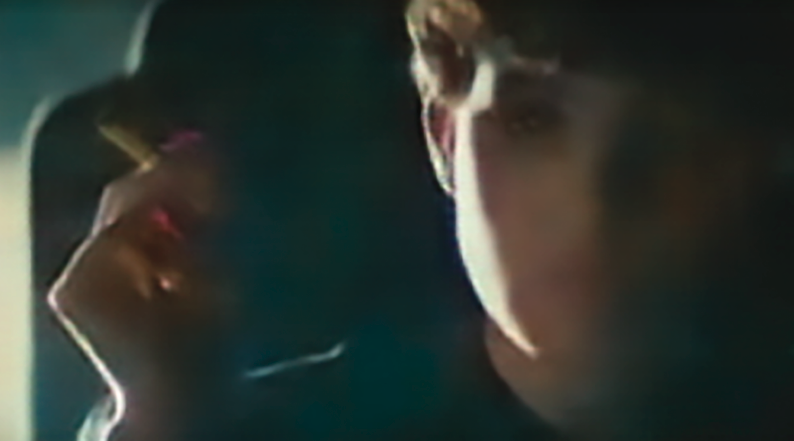
\includegraphics[width=1\textwidth]{figures/c1_intro/blade_runner_still.png}
    \caption{Still from \textit{Blade Runner --- Autoencoded}.}
    \label{fig:c1:blade-runner}
\end{figure}

The training data, of course, was not intellectual property that I had permission to use.\footnote{It should also be noted that I was not even the first person to recreate \textit{Blade Runner} with machine learning. Ben Bogart's work \textit{Watching (Blade Runner)} was also created in 2016 \citep{bogart2016watching} (and built upon earlier research \citep{bogart2008memory,bogart2013context}), which I only learnt of its existence many months after completing my own recreation of the film.}
Ironically, this project and the resulting (and later rescinded) DMCA copyright takedown notice given to the videos on the web platform Vimeo was what catapulted the work to international recognition after an account of these travails was detailed in the news website Vox \citep{romano2016bladerunner}.

\begin{figure}[!htb]
    \centering
    \captionsetup{justification=centering}
    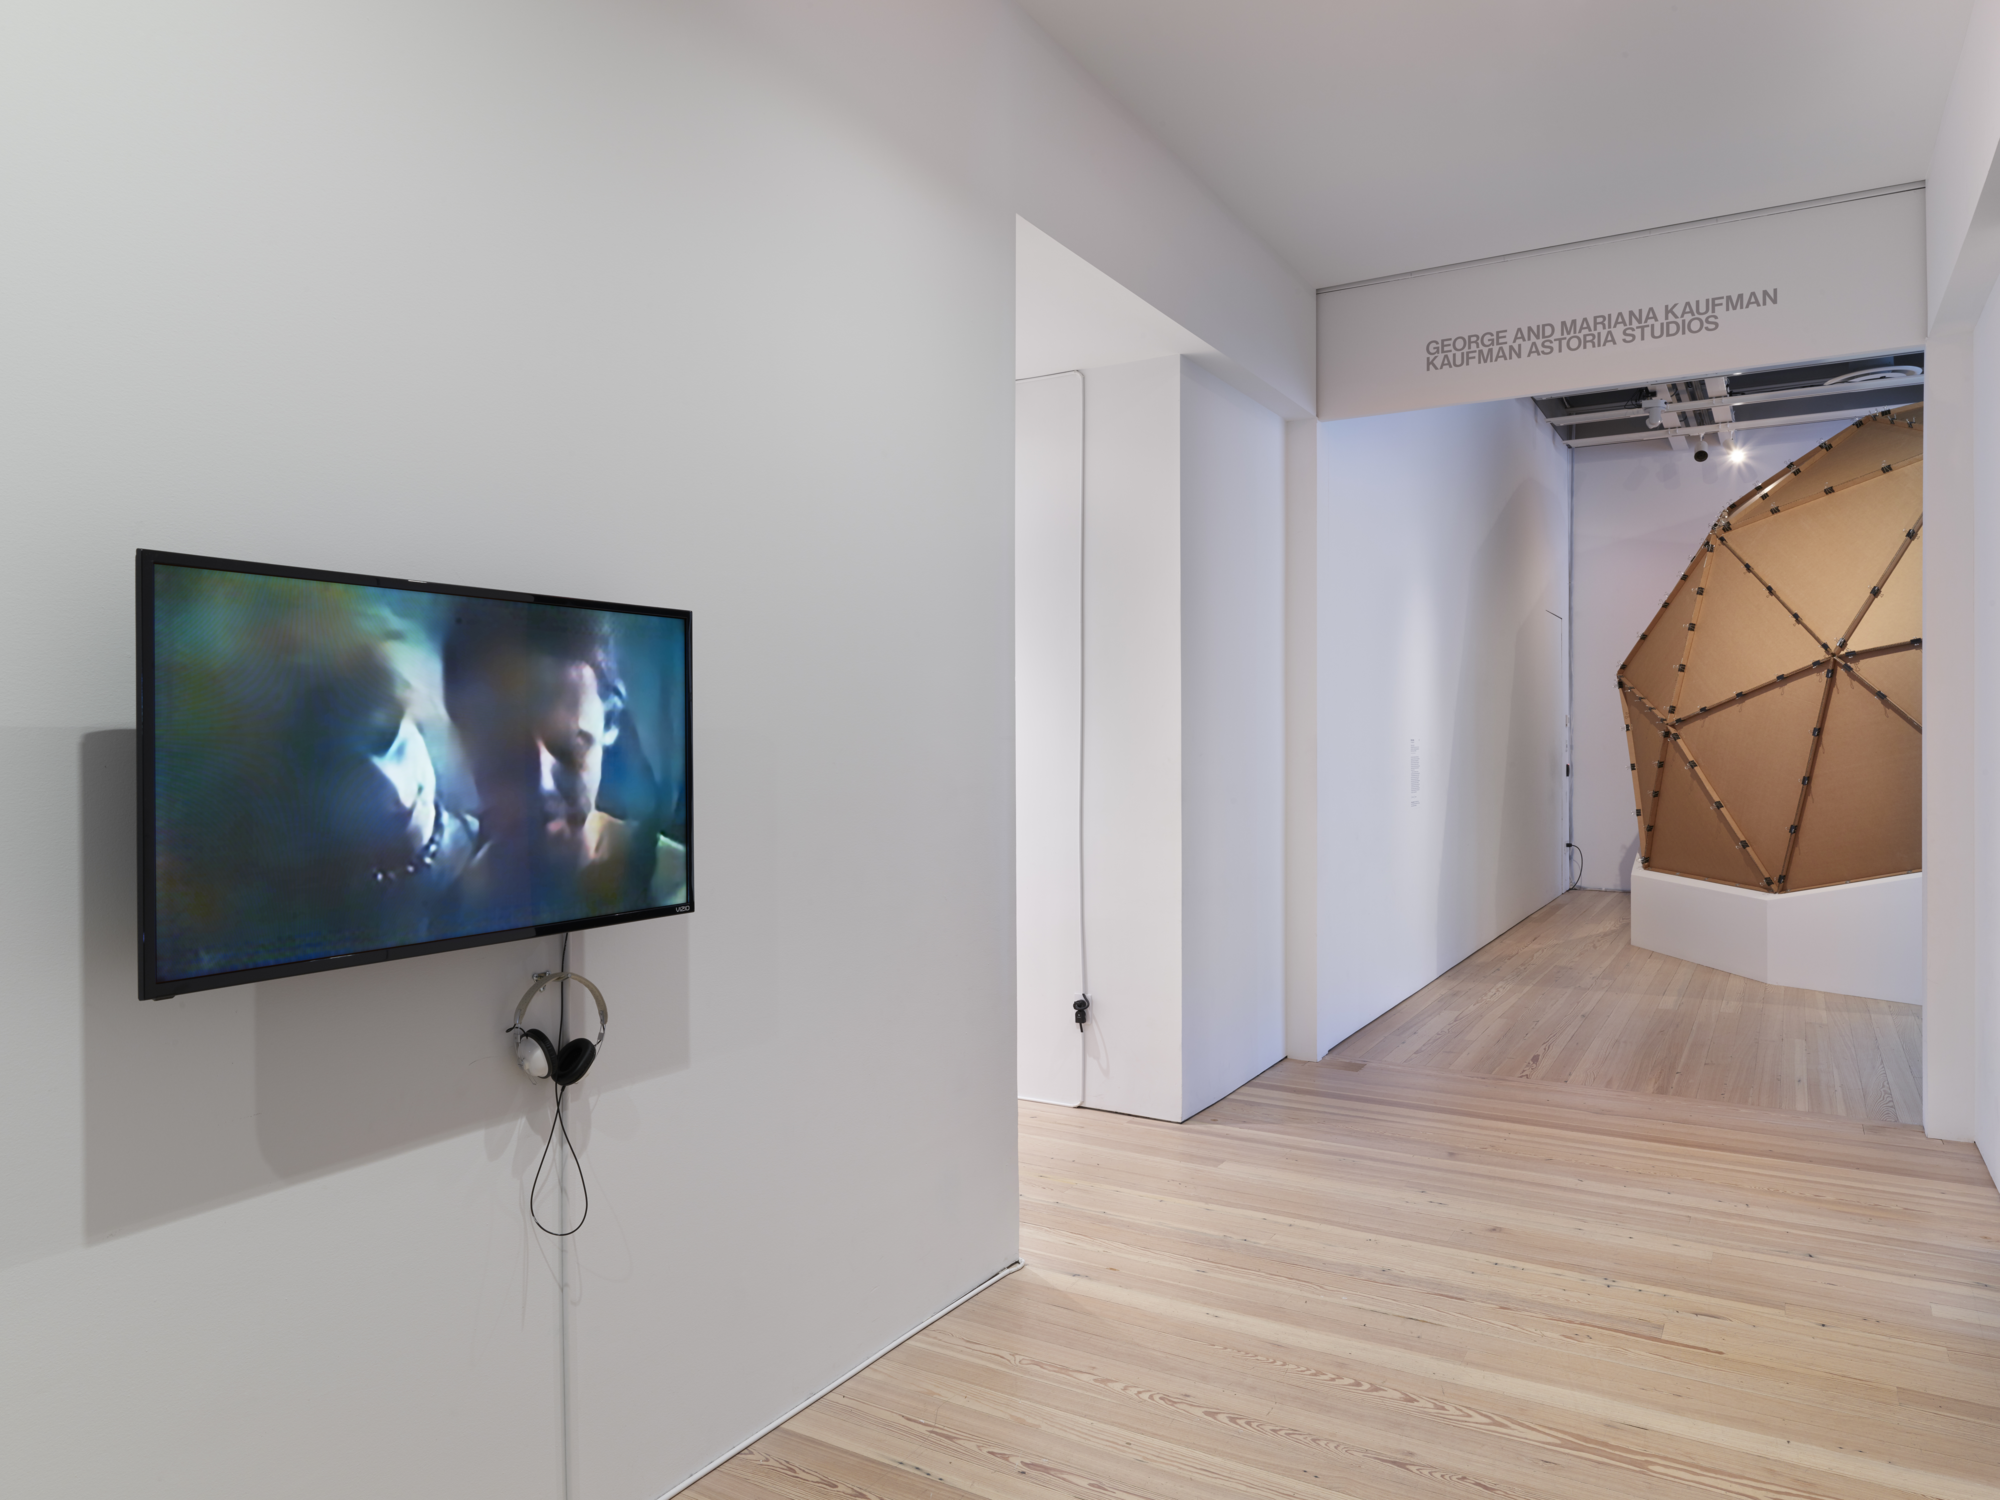
\includegraphics[width=1\textwidth]{figures/c1_intro/whitney-installation-shot.png}
    \caption[Installation view of \textit{Blade Runner --- Autoencoded} at the Whitney Museum of American Art]{Installation view of \textit{Dreamlands: Immersive Cinema and Art, 1905-2016} (Whitney Museum of American Art, New York, October 28, 2016-February 5, 2017). Left to right: Terence Broad, \textit{Blade Runner - Autoencoded}, 2016; Liam Gillick, \textit{Annlee You Proposes}, 2001. Photograph by Ron Amstutz. Image courtesy of the Whitney Museum of American Art.}
    \label{fig:c1:blade-runner-whitney}
\end{figure}

Though I did not face any further legal action from Warner Brothers for  disseminating the work, it was a major cause of personal stress, as I was very often anticipating some form of legal intervention (e.g. a cease and desist notice) from Warner Brothers prior to any exhibition where the work was going to be shown.
An opinion published in the Columbia Journal of Law and the Arts predicted that the work would probably be dealt with as copyright infringement were it tested in an American court \citep{sobel2017artificial}.\footnote{An alternative legal opinion was given by legal scholar Andres Guadamuz, who believed that this would be protected by fair-use or fair-dealing if it were to be tested in court on the basis of parody or pastiche \citep{guadamuz2024personal}.} 
I produced the work before the widespread emergence of NFTs and before there was a large market for AI-generated artworks. 
The money I made from exhibition fees and selling editions of the video work would have been relatively insignificant for a multinational media company. 
Nonetheless, this experience was instrumental in informing the subsequent research presented in this thesis. 
Finding ways of using generative AI that does not rely on data and the intellectual property of others was a key aim for the research presented in this thesis.


\section{Motivation}

My goal was to find ways of training or configuring generative AI models which did not rely on the creation of datasets to produce creative outcomes. 
From working in the AI industry, I had experienced how labour-intensive and time-consuming creating high-quality datasets could be, and it was clear this was a hugely time-consuming aspect of Generative AI research processes.
The second was to find ways of achieving novel outcomes that did not rely on access to high-end resources, for example, those available to large technology companies, including Google DeepMind, NVIDIA, or artists such as Refik Anadol (who reportedly have access to considerable computational resources  \citep{caulfield2022refik}). 
To this end, this research has focussed on exploring methods for training, configuring and customising very high-fidelity models that, when trained conventionally, require supercomputer-level resources. 
As such, this thesis presents a number of useful methods for manipulating, training and controlling these same models in much shorter time periods on consumer-level hardware.

Instead of relying on laboriously or ethically questionable datasets to try and achieve creative outcomes, the work in this thesis details data-free methods that push the possibility space of what can be generated with contemporary neural networks.
The approaches detailed are an attempt to use the intrinsic affordances of these neural networks to create original outputs that would not have been possible using any other technique or technology. 
The work detailed in this thesis is experimental image-making in its truest sense, and I have taken more inspiration from experimental photographers and filmmakers of the 20th Century (such as Harold Edgerton, Hiroshi Sugimoto, and Oskar Fischinger) than from academic researchers.

The driving force that led to each technical breakthrough in this thesis has been technical curiosity. 
When considering a new possible configuration for training an AI or some other kind of intervention, if I couldn’t imagine what the result of that experiment would look like, I would have to build it to find out, regardless of how many weeks or months of work it would take to get there. 
The results presented here are the experiments that produced the most surprising and striking results - sometimes beautiful and sometimes horrifying. 
There were a lot of failed experiments along the way that produced boring, predictable and uninspiring results. 
I’ve spared the reader details of most of these, apart from the few that led to key insights.

\section{Research Methods}

The research breakthroughs presented in this thesis have all come from a technological exploration of what is possible with these new technologies. Much of this research has been conducted in the vein of hacking, in its original meaning from the hacker culture at MIT (Massachusetts Institute of Technology) in the 60s and 70s, where hacking meant `exploring the limits of what is possible, in a spirit of playful cleverness' \citep{stallman2002hacking}. 
This hacking ethos is not an approach that many people were taking in machine learning research when I started this PhD. 
The field was, and still is, very much dominated by orthodoxies and ideology, where theoretical mathematical underpinnings, achieving state-of-the-art performance on some widely used benchmark, and generalisation are most valued by the research communities \citep{birhane2022values}.

\textit{Hacking} was the primary means by which the algorithms in this thesis were discovered, but artistic exploration has also been central to the experimental work described in this thesis. 
When I started this PhD, my plan was to conduct primarily technical research and continue with an artistic practice on the side, maybe using some of the techniques developed in my research. 
Instead, it was an artistic enquiry that led me to the technical breakthroughs in the PhD, not the other way around. 

In his paper \textit{`Art in the sciences of the artificial'}, Stanley argues that in the fields of AI research and artificial life, subjective evaluation is a key driving force of progress for many researchers and practitioners in the field. 
There is a tendency in these research fields to discourage the dissemination of these observations in academic writing and in wider public discourse, something that Stanley worries might `cut off some future discoverers from what could have been their inspirations' \citep{stanley2018art}. 
In this thesis, I have sought to share my subjective position at various times in the thesis, and how that informed the direction of the following research experiments (\S \ref{c8:sec:aesthetic} for a further reflection on this).

Being both guided by, and disseminating this kind of subjectivity is commonplace in research practices in many areas of the humanities, including research methods such as autoethnography \citep{reed1997auto}, or practice-based and practice-led research \citep{candy2006practice}. 

The goal of this research has been at its core, to advance the creative possibilities of these technologies. 
As a practising and internationally recognised visual artist, my subjective understanding of the visual potential and aesthetics of these systems has been one of the central guiding instruments in this research. 
To give any other account of how this research was conducted would be a failure of academic integrity. 

The work  I have done that is described in this dissertation and the contributions made in this thesis were the outcomes of practice-led research. 
The artistic outcomes are not presented as contributions to be assessed as outcomes of the thesis as such, but the process and practice that went into making them are described in an honest account in this thesis. 
Descriptions of artworks that have been made by myself and others using the techniques that have been described in this thesis are detailed in Chapter \ref{ch:impact}.

\section{Overview and Contributions of the Thesis}

The thesis is entitled \textit{Expanding the Generative Space}. 
The throughline of all of the research presented here has been to find ways of going beyond the imitation of training data as the sole method for training generative neural networks. 
Instead, I have been trying to expand the possibility space that generative AI can produce, and the methods described in this thesis are but a few of the ways that this is possible. 

\subsection{Background}

Chapter \ref{ch:background} provides a thorough review of relevant background literature and related research conducted prior to the work presented in this thesis.
This review encapsulated both the technical aspects of machine learning relevant to this thesis, and also its application in creative contexts, whilst also drawing on the broader history of AI methods such as evolutionary algorithms, and their applications for generative processes. 
This chapter also describes notable prior work in relation to attempts to achieve novel outcomes with generative neural networks.

\subsection{Training without Data}

Chapter \ref{ch:unstable_eq} documents the first peer-reviewed and published approach to training generative neural networks without data, one of the three categorical contributions to active divergence methods (\S \ref{survey:nodata}) presented in this thesis.
This work was first published in the paper \textit{`Searching for an (un)stable equilibrium'}: experiments in training generative models without data' at the NeurIPS 2019 Workshop on Machine Learning for Creativity and Design \citep{broad2019searching}.

\subsection{Divergent Fine-Tuning}

Chapter \ref{ch:divergent} documents the first peer-reviewed and published approach to divergent fine-tuning of generative AI models without relying on imitation-based learning.
Divergent fine-tuning is another categorical contribution to active divergence methods (\S \ref{survey:divergent}) presented in this thesis.
This work was first published in the paper \textit{`Amplifying the uncanny'} at the 8th Conference on Computation, Communication, Aesthetics \& X (xCoAx) \citep{broad2020amplifying}.


\subsection{Network Bending}

Chapter \ref{ch:net_bend}, presents the network bending framework and is the third categorical contribution to active divergence methods presented in this thesis (\S \ref{survey:bending}).
This work was first published in the paper \textit{`Network Bending: Expressive manipulation of deep generative models'} at the International Conference on Artificial Intelligence in Music, Sound, Art and Design (EvoMUSART) \citep{broad2020network}, and later extended in the paper \textit{`Network Bending: Expressive Manipulation of Generative Models in Multiple Domains'} for the journal Entropy \citep{broad2021network}.
Network bending has been widely reused and adopted by many other artists and researchers (detailed in \S \ref{c7:sec:net-bend-artworks} \& \S \ref{c7:sec:net-bend-impact}).

\subsection{Active Divergence Taxonomy}

The final contribution of this thesis is the survey and formal taxonomy. 
The large majority of experimental work in this thesis falls under the umbrella term \textit{active divergence}. 
This was first coined by a PhD colleague and friend, Sebastian Berns and his supervisor Simon Colton [\citeyear{berns2020bridging}]. 
The core experimental work in this thesis pre-dates this definition, and I am indebted to Sebastian for summarising the overarching theme of my research, which felt far more disparate when I was working on it until he was able to summarise it in a two-word definition. 
In collaboration with Sebastian and Simon, I expanded on this definition and the paper \textit{`Active Divergence with Generative Deep Learning - A Survey and Taxonomy'} at the International Conference of Computational Creativity in 2021 \citep{broad2021active}.
An updated summary of that survey is presented in Chapter \ref{ch:active_div} and details work completed concurrently by others during the time of this PhD to achieve similar goals.

\subsection{Impact and Discussion}

Chapter \ref{ch:impact} details the impact of the research presented in this thesis and the subsequent work that this thesis went on to inspire. Chapter \ref{ch:discussion} reflects on the work undertaken, how artistic approaches to hacking AI models and training can lead to new forms of understanding, and how AI itself can be used as a material for artistic exploration and expression, a topic that I discussed in the paper \textit{`Using Generative AI as an Artistic Material: A Hacker's Guide'} that I presented at the 2nd international workshop on eXplainable AI for the Arts (XAIxArts) at the ACM Creativity and Cognition Conference \citep{broad2024using}.

\subsection{Conclusion}

Chapter \ref{ch:conclusion} concludes the thesis and reflects further on its contributions.
This chapter also details the limitations of the research presented in this thesis and discusses possible future research directions to take this work further.

\section{Summary}

In the six years that I have been working on this PhD, there has been a huge amount of upheaval in the research field and its impacts on wider society. 
I have seen AI art and generative AI go from a small, quirky community of enthusiasts to a booming industry that has become pitted against the interests and livelihoods of the creative professionals that they are extracting value from.
Hopefully, the approaches to working with AI described in this thesis can help others to find ways of using and working with generative AI which does not rely on the mass stealing and exploitation of creative professionals but instead fosters new ways for creative people to use generative AI in ways that creative people will always do: to deliberately break, misuse and adapt technologies far beyond the intended purpose to forge new forms of creative expression.


\chapter{Background}
\label{ch:background}

\section{Introduction}

This chapter serves as a survey of relevant background literature predominantly available prior to me undertaking my experimental research.
The majority of the chapter outlines the technical basics of machine learning, neural networks and generative modelling.
Further, the chapter also describes relevant research conducted in areas including computation, creativity, generative systems and divergent thinking prior to the advent of deep learning circa 2011-12 \citep{krizhevsky2012imagenet}.

\section{Computation \& Creativity}

Since the advent of automated computing machines, and the idea of writing programs to give these machines instructions to follow, the idea of using computers to develop artefacts deemed creative has been long imagined. 
Ada Lovelace, the woman considered to be the first ever computer programmer, imagined that programmes for Charles Babbage's unfinished Analytical Engine could ‘compose elaborate and scientific pieces of music of any degree of complexity or extent’.
Lovelace however, did not think that computers could originate creativity themselves, declaring ‘The Analytical Engine has no pretensions whatever to originate anything. I can do [only] whatever we know how to order it to perform.' \citep{lovelace1843notes}.

Alan Turing took an opposing viewpoint to Lovelace on this question, stating that this objection would be better posed as ‘a machine can never take us by surprise’, countering that ‘Machines take me by surprise with great frequency [...] because I do not do sufficient calculation to decide what to expect them to do.’ \citep{machinery1950computing}
This reframing from originality to surprise shifts the emphasis from an action by the machine to an evaluation based on a human reaction. 
Turing develops this further, by describing a scenario called \textit{The Imitation Game}, where a computer would be evaluated through a text channel and asked questions by an evaluator who would then attempt to differentiate whether it was human or not. 
If the evaluator considered the computer output to be from a human, this would be a threshold for determining simulated intelligence.
This method for evaluating computational intelligence is commonly referred to as the Turing test. 

In his description of the imitation game, Turing took seriously the idea of a computer being able to develop creative work. 
In the paper \textit{`Computing Machinery and Intelligence'} he muses about a machine writing a sonnet, and then, through the viva voce style of examination, being able to critically defend the work against a human interrogator based on criteria of aesthetic value, originality and of potential subjective readings of proposed changes to the language used in the work \citep{machinery1950computing}.

The idea that the bar for Artificial Intelligence (AI) is to convincingly imitate human behaviours, is one that has long been an anchor for research in the field. 
Imitation is central to much of how we train machine learning, neural networks and generative models, importantly imitation alone is not broadly considered a benchmark for intelligence.
An alternative theoretical test for computational intelligence is the Lovelace test, where a computational program would pass the test a) it can generate an original artefact (poem, musical score, novel, idea) that can be reproduced and b) the creators of the program can not explain how it has found that solution \citep{bringsjord2003creativity}. 

\cite{ward2020computational} argues that Turing's characterisation of Lovelace's lack of faith in the possibility for the analytical engine to produce origination (that he equates with surprise) is a mischaracterisation and misunderstanding of the debates around mechanisation and origination that were happening during the industrial revolution. 
In the same notes where she makes her famous objection, she also goes on to say that the analytical engine has the power to offer new perspectives by combining theories in new ways \citep{lovelace1843notes}.
 Lovelace's remarks demonstrate the creative value of human-machine interaction, where she `understand[s] mechanicity not as inherently creative or uncreative but as a mode through which new kinds of creativity are possible' \citep{ward2020computational}.

\subsection{Theories of Creative Processes}

Creativity itself is broadly agreed as a well-defined concept, though there are some differences in definition. 
Narrower definitions of creativity refer to the cognitive processes involved in culturally understood creative activities, such as 'pieces of music, sculpture, painting, poems or other things that are taken or presented as art' \citep{wiggins2015evolutionary}.
Creativity though, is used much more broadly in common language. 
It can also be applied to acts, ideas or behaviours outside of the realm of art-making, such as scientific fields, sports, economic activities or even mundane, day-to-day activities.


A broader definition of creativity is that it is an act that produces something \textbf{new and original} \citep{kaufman2021overview}. This act needs to be task-appropriate, fulfilling the requirements of whatever the original task set out. 
However, theories of how creativity is achieved, what facilities it, and how it is recognised and evaluated are far more disparate and less agreed upon. 

Theories of what makes a person creative tend to focus on a summation of different elements.
The componential model of creativity proposes that three interconnected variables are key to individual creativity.
First, there are domain-relevant skills and knowledge, such as a technical skill or specific talent.
Secondly, there are skills relevant to creative processes, such as a tolerance for ambiguity and a willingness to take certain risks.
Finally, intrinsic motivation is needed to take part in an activity because it is enjoyable and meaningful \citep{amabile1983social}.

There are many other theories of creativity, pertaining to evaluating individual persons' creativity, creative collaborations, understanding traits of creative peoples and situations that best facilitate creativity and how creativity is evaluated from a historical or cultural perspective. 
The outline in the rest of this section will only cover theories or models of creative processes which have been developed in order to understand how to enhance and replicate creative acts, and in some cases, so that they can be partially or fully automated with computation.

\subsubsection{Convergent and Divergent Thinking}

The psychologist J.P. Guilford set out a series of traits and cognitive processes specific to creative activity. Those are ideation fluency, ideation novelty, synthesising ability and redefining ability, sensitivity to problems and evaluating ability \citep{guilford1950creativity}. 
The fluency with ideas generated, the novelty of said ideas and the ability to then critically evaluate those ideas and pick the best one are some of the most important traits for creative people.\footnote{Notably, Guildford motivates this early research into the psychology of creativity because of the rise of \textit{thinking machines} (aka digital computers). Imagining their eventual knock-on effect on the labour market and a future industrial revolution of intelligence being automated, Guildford muses that the only economic value left of human brains would be in the creative thinking they are capable of \citep{guilford1950creativity}. A viewpoint I am not unsympathetic to.}

Guilford later builds on this theory, expanding the thinking processes needed in creative thinking, in particular the processes that are required for the production of creative ideas.
He differentiates two kinds of productive thinking that are required for creativity; divergent and convergent thinking. 
Convergent thinking is the focusing of ideas down to a single correct answer. 
Divergent thinking is the diametric opposite, which is the ability to generate new and different ideas. 
In the context of modelling creative acts, these two types of thinking are also called idea generation and idea evaluation \citep{guilford1957creative}.

Of these two modes of productive thinking, Guilford believes divergent thinking is that which is more representative of and unique to the creative process. 
He considers factors of fluency, flexibility and original thinking as products of abilities in divergent thinking.
Guilford's ideas about divergent thinking went on to inspire many other aspects of research, such as the Torrance test for creative thinking \citep{torrance1966torrance}.

\subsubsection{Associative Creativity}

Associative creativity is the theory that creative people or creative acts are made when connections are made between remote concepts or ideas \citep{mednick1962associative}. 
Koestler coined the term \textit{bisociation} to describe a cognitive process where two or more concepts are combined to create a new concept \citep{koestler1964act}.
This model of creativity is also referred to as \textit{combinatorial creativity} \citep{boden2004creative}.

\subsubsection{Evolutionary Theory of Creativity}

Evolutionary theory states that the genetic structure of living beings is constantly changing through processes of random mutation and selection. Selection is carried out in two ways: \textbf{natural selection} is the process of fitness through living beings surviving long enough to reproduce sexually and transmit their genome. \textbf{Sexual selection} is the process by which organisms make preferential choices regarding which partners to mate with based on particular attributes.

An evolutionary approach to how ideas are generated and selected in creative acts was proposed by \cite{campbell1960blind}, where he stated that the process of blind variation and selective retention in thought achieves innovation (aka creativity).
According to Campell, this occurs through the internal emitting of thoughts, a process which lacks prescience and foresight.
Campbell justifies this as a blind process, stating that `once the process has blindly stumbled into a thought trail that ``fits'' the section criterion, accompanied by the ``something clicked'' or ``Eureka'' that usually marks the successful termination of the process' \citep{campbell1960blind}.

\subsection{Computational Creativity}

Computational creativity is a subfield of AI research which investigates developing software that exhibits creative behaviours which unbiased observers would perceive as being creative \citep{colton2012computational}.
Computational creativity research is usually preoccupied with artefact generation in domains that are culturally recognised as being creative, such as poetry, story generation, images or music.
The mechanics of the system and how they are constructed to imitate the creative faculties of humans is the central area of exploration, whereas the quality of the generative process and the outputs from them is usually a secondary concern.

Computational creativity differentiates itself from the practice of building and evaluating creativity support tools, such as those commonly researched in the field of HCI (Human-Computer Interaction) (\S \ref{c2:subsec:cst}).
Famously, the tagline at the 3rd International Conference on Computational Creativity in 2012 was ‘scoffing at mere generation for more than a decade’, though this has become an increasingly divisive phrase within the computational creativity community \citep{ventura2016mere}.

\subsubsection{Human-AI Co-Creation}
\label{c2:subsubsec:co-creativity}

Human-AI co-creation (also referred to as co-creativity) is a subfield of computational creativity research where the creative responsibility is shared between the software and the human interacting with it \citep{candy2002modeling}.
This framing positions the software as a creative collaborator, as opposed to an independent creative agent or tool only for supporting human creativity \citep{feldman2017co}.

\subsection{Metacreation}

Metacreation is the practice of developing software that demonstrates creative behaviour \citep{whitelaw2004metacreation}. 
In metacreation practice, the objective is not just to develop software, but to produce and present artistic works derived from the software, to validate their success. 

\cite{eigenfeldt2012evaluating} describe five viewpoints that should be considered when evaluating a metacreation system: (1) the designer of the system, (2) the audience for the derived artworks, (3) academic experts, (4) domain experts, (5) results from controlled experiments.
This emphasis on audience evaluation and domain expertise differentiates metacreation research from computational creativity, where the emphasis is in the inherent soundness of the processes encoded in the system architecture \citep{colton2008creativity}.

\subsection{Creative Computing}

Creative computing is an academic discipline\footnote{Creative computing is the academic discipline I am most at home with, having done my BSc and (integrated) Msci in Creative Computing at Goldsmiths, University of London, and more recently, being employed as a Senior Lecturer at the Creative Computing Insititute at University of the Arts London.}
that builds from the alternative computing scenes of the latter half of the 20th Century, which include \textit{hacking} and \textit{the demoscene}. 
Hacking and the creation of a \textit{hack}, is a specific sense of creative invention with given materials in the context of electrical engineering and the academic environments researching this in the 1960s in MIT and Stanford \citep{wark2006hackers}. 
Though not exclusively used to describe computer code or a technical system, a hack had to `be imbued with innovation, style and technical virtuosity' \citep{levy1984hackers}.

Hacking later became associated with the breaking of digital security and performing acts of digital trespassing and accessing confidential information, a practice that has retrospectively been called cracking. 
Cracking copy protection on home computer systems, for the distribution of games led to the evolution of the demoscene. 
 In the demoscene, visual and audio programs were written and freely shared, where value was determined, for example, as follows: ‘more graphical elements, more mathematical effects and more sounds made a better demo, while bugs, glitches, and irregularities made the demo worse’ \citep{carlsson2019forgotten}.

Creative computing refers to the practice of using computing technologies to create expressive artefacts rather than something that is strictly functional \citep{yang2016promoting}.
In creative computing, programming is the main tool that the creator uses to generate an artefact, and coding is the medium used to express human creativity. 

Creative coding is often carried out with creative coding frameworks, which are libraries, programming languages, or visual programming interfaces (such as node-based programming). 
Creative coding frameworks tend to focus on supporting visual rendering, audio processing and supporting human interaction with these frameworks. 


\subsection{Creativity Support Tools}
\label{c2:subsec:cst}

Creativity support tool (CST) is the term given to software programs that are designed to facilitate creative acts or enhance a user's creativity \citep{shneiderman2002creativity}. 
For CSTs, the graphical user interface (GUI) is of high importance \citep{shneiderman1999user}. 
CSTs can be used to facilitate many varieties of tasks such as searching, visualising, consulting, thinking, exploring, composing, reviewing and disseminating \citep{shneiderman2002cst_tutorial}.

With creativity support tools, the code is neither seen as acting in a creative way in its own right nor is it a medium for humans to be creative. 
Creativity support tools are independent pieces of software that can facilitate creativity but are not seen as being responsible for contributing to the creative process in their own right, as is the case with human-AI co-creativity (\S \ref{c2:subsubsec:co-creativity})

\subsection{Computational Models of Creative Processes}

There is a large existing literature on computational models that encode specific theories of creative processes, or specific attributes that are deemed essential for creative people to have.
This subsection covers a non-exhaustive selection of these methods described in the literature.

\subsubsection{Evolutionary Computation}

Evolutionary computation refers to algorithms that are inspired by the process of biological evolution to perform some form of optimisation. 
The most commonly used evolutionary algorithm is the \textit{genetic algorithm}, which is inspired by many of the processes present in biological evolution, such as random mutation, sexual selection, or (chromosomal) crossover.

Genetic algorithms require some kind of \textit{fitness function}, that determines the quality or performance of an individual solution to whatever optimisation problem is trying to be solved. 
This is analogous, and in some ways similar to the \textit{loss functions} used in machine learning algorithms (\S \ref{c2:sec:ml}). 

A genetic algorithm requires a genetic representation of the solution domain. 
This representation is usually a linear vector, and is often binary, with a fixed length representation, which allows for easy implementation of genetic operations such as crossover. 
The parameters in the genetic representation need to be carefully selected as they determine the \textit{solution space}.
Genetic algorithms are a stochastic optimisation process for exploring a \textit{fitness landscape} and converging onto a high-quality solution \citep{back1996evolutionary}.

\subsubsection{Novelty Search}

Novelty search is an algorithm developed by \cite{lehman2008exploiting}, first used to guide evolutionary algorithms, where there is no set objective or fitness function.
Instead, the search for novelty in the behavioural space of an evolutionary agent is the sole criterion. \cite{lehman2010efficiently, lehman2011abandoning,lehman2011novelty} argue that by abandoning prescriptively defined objectives, novelty search algorithms can better search the possibility space of an evolutionary landscape, and they show that this approach can lead to both unexpected and more optimal behaviours in evolutionary agents.
This approach to open-ended learning in evolutionary algorithms has inspired more recent developments in the space of open-ended reinforcement learning \citep{wang2020enhanced} (\S \ref{c2:subsec:reinforcement} for a definition of reinforcement learning).

\subsubsection{Bayesian Surprise}

Bayesian Surprise \citep{itti2005bayesian,itti2009bayesian} is an algorithm that takes inspiration from information theory and Bayesian statistics, that gives a mathematical formulation for surprise. 
This computational measure closely correlates with human attention, through the measurement of gaze shift of human participants watching television broadcasts.

\subsubsection{Intrinsic Motivation}

In agent-based AI modelling, intrinsic motivation is defined as goals or objectives for the agent that are not determined by external stimuli or reward functions (aka external motivation), but by the internal state of the agent itself. 
Intrinsic motivation can be applied in reinforcement learning agents \citep{chentanez2004intrinsically} (\S \ref{c2:subsec:reinforcement}), and is motivated by the proposition that not all objectives are universally useful \citep{barto2013intrinsic}.
Intrinsic motivation in AI is grounded in evolutionary theory \citep{singh2010intrinsically}, where an otherwise single mathematical function that defines a universal fitness function does not account for all behaviours and evolutionary strategies exhibited in real-world biological evolution.

\subsubsection{Compression Progress}

Compression progress \citep{schmidhuber2008driven} is a theoretical approach to training agents that relates to novelty search \citep{lehman2008exploiting} and intrinsic motivation in RL agents \citep{chentanez2004intrinsically}.
Schmidhuber defines compression progress as an agent that is constantly trying to efficiently represent prior actions in an environment, whilst constantly seeking out new experiences that would satisfy an `intrinsic curiosity reward', which would drive the agent toward seeking out novel and unpredictable experiences.
Schmidhuber argues that this framework could be used for mathematical discovery, as well as art-making through `subjective beauty'.

\subsubsection{Combinatorial Creativity}

Combinatorial creativity is the description of a creative process where two or more concepts are combined together to make new ones \citep{boden2004creative}. 
This concept is essentially a rehashing of the concept of bisociation first proposed by \cite{koestler1964act}. 
Combinatorial creativity has been explored extensively in the context of computational creativity research \citep{zarraonandia2017using, guzdial2018combinets, guzdial2018combinatorial} and in explaining the psychology of scientific discovery \citep{simonton2021scientific, simonton2022serendipity}.

\subsection{Enacting Creative Processes in the Computational Arts}

Many artists have explored models of creativity and creative processes through practice-based enquiry.
Artists have made substantial contributions to this field and our understanding of non-human creativity, and the interactions between people and computers in exploring new possibilities for creative autonomy and creative collaboration.
A selection of these efforts is detailed in the following.

\subsubsection{Human-AI Co-Creation}

Harold Cohen, the pioneering computational artist, developed and worked with the AARON program and robotic painter (using an XY plotter), to co-create paintings between 1972-2010 \citep{cohen2016harold}. 
The program underlying AARON was developed by Cohen himself \citep{cohen1995further}, using deterministic software that was in a constant process of development. 
AARON has been described as a form of meta-art (or metacreation) \citep{mccorduck1991aaron}, where the artwork itself is the creation of a process that creates art.

The artist Sougwen Chung extends Cohen's work to create a practice that is centred around performative works where Sougwen collaboratively and interactively \citep{benediktsson2019human}.
Sougwen uses this practice to explore themes of increasing automation and co-existence between humans, algorithms and machines \citep{voss2021conversation}.

\subsubsection{Evolutionary Arts}

Many artists have explored the biological theory of evolution and evolutionary computation for artistic experimentation.
Karl Sims seminal experiments explored evolutionary computation for the creation of computer graphics \citep{sims1991artificial} and 3D morphology and behaviours in artificial creatures \citep{sims1994evolving, sims2023evolving}.

The artist William Latham, alongside collaborator Stephen Todd, developed the FormGrow to evolve 3D computer models resembling organic life \citep{latham1992evolutionary}, with the aesthetic preference of the artist guiding the evolutionary process \citep{lambert2013emergence}.
Using aesthetic preference to guide evolutionary systems was also utilised in the work \textit{Cellular Forms}, where \cite{lomas2014cellular} built his own user interface to interactively explore the possibility space of simulations of growing cellular organisms.

\section{Machine Learning}
\label{c2:sec:ml}
Machine learning algorithms are algorithms that automatically improve from training data or experience. 
Given training data, a machine learning algorithm will build a model to make predictions or decisions without explicitly being told what decisions to make. 
Most machine learning algorithms use some form of optimisation and are optimised to minimise a loss function that is generally predetermined and task-specific. 
The process of optimising a machine learning model is referred to as \emph{training}. 
When training a machine learning model, the loss function on the training data will be minimised with the goal of maximising the accuracy for the specific task. 
The model is generally evaluated on a separate test dataset that contains data not used during the training phase \citep{murphy2012machine}.

\subsection{Supervised Learning}

Supervised learning algorithms build models based on training data that contain the desired set of output and inputs. 
This type of training data is referred to as \emph{labelled data}. 
A labelled dataset will consist of pairs of data, where every input will be given with a corresponding output. 
Labelled datasets are in most cases hand-labelled by human users who ideally have expertise in the subject domain.
Three of the most common tasks in supervised learning are \emph{classification}, \emph{regression} and \emph{metric learning}. 


\subsubsection{Classification}

In classification, each data sample $x$ will be paired with a vector $c$ that represents the class label. 
The machine learning model will take $x$ as an input and output a prediction $c'$. 
The objective during training is to maximise that the probability of the prediction $c'$ will match the value of the true label $c$ \citep{murphy2012machine}. 

\subsubsection{Regression}

In regression, each data sample $x$ will be accompanied by an output $u$, where the output values are numerical values within a given range. 
The model will learn to output predictions $p'$ for input $x$. The goal of training a regression model is to learn a model that can generalise to unseen data, where the input and output values are not necessarily present in the training data but can be inferred based on the examples given in the training data \citep{murphy2012machine}. 

\subsubsection{Metric Learning}
\label{c2:subsubsec:metric}

The goal of metric learning is to learn a distance function between given samples, that can be used to estimate how similar or dissimilar samples are. 
The model learns to provide a distance function $d(x,y)$ for input examples $x$ and $y$. In the labelled dataset, input examples are usually accompanied by a vector label $c$ donating the identity of the input example. 
When training a model, the goal is usually to minimise the distance between samples that have the same identity but maximise the distance between samples that have separate identities \citep{kulis2013metric}.

\subsection{Unsupervised Learning}

Unsupervised learning algorithms find patterns in data where there are no given labels. 
Unsupervised learning methods find patterns and structures within data without guidance, either by learning discriminative features or capturing patterns as probability densities. 
The two most common tasks in unsupervised learning are \textit{clustering}, \textit{dimensionality reduction} and \textit{generative modelling}.

\subsubsection{Clustering}

Clustering is the task of grouping data into clusters such that data grouped together in the same cluster are more similar to each other than data in another cluster. 
Examples of algorithms used for clustering are K-means, Gaussian mixture models or density-based clustering methods \citep{xu2005survey}.

\subsubsection{Dimensionality Reduction}

Dimensionality reduction is the task of transforming high-dimensional data into a lower-dimensional representation that still retains key characteristics present in the original data. 
Examples of algorithms used for dimensionality reduction are Principle Components Analysis (PCA) \citep{pearson1901liii}, t-Distributed Stochastic Neighbour Embedding (t-SNE) \citep{hinton2002stochastic} and autoencoders (\S2.2.1). 

\subsubsection{Generative Modelling}

Generative modelling is the task of learning a function that can generate a given data distribution. 
A generative model will give a joint probability distribution between the observable and target variables. 
Approaches to generative modelling include Gaussian mixture models, hidden Markov models and neural networks. 
An overview of generative model approaches using deep neural networks is given in Section \ref{c2:sec:gen-nn}.

\subsection{Reinforcement Learning}
\label{c2:subsec:reinforcement}

Reinforcement learning (RL) is a form of agent-based modelling, where the agent learns how to behave in an environment by performing actions and receiving feedback in the form of penalties or rewards \citep{sutton1999reinforcement}. 
The most commonly used algorithm in RL is Q-learning, where the agent learns the value of taking a specific action in a specific state in the environment \citep{watkins1992q}.
Over the course of learning, a Q-table matrix records values for each state-action pair and gradually improves the policy.

\section{Artificial Neural Networks}

Artificial neural networks are ensembles of connected units that are meant to loosely model the synaptic structure of biological neural networks. 
The first artificial neural network was the Mark 1 Perceptron \citep{rosenblatt1958perceptron}, initially a physical circuit that was designed to perform the binary classification of images captured from a sensor array. 
The values of the weights between connections were encoded using potentiometers with a learning rule updated with electric motors. 
Later the perceptron architecture was modelled in software rather than hardware, with weight parameters and values encoded as real-valued numbers. 
The term perceptron was later used to denote a unit (or node) within a larger network and is used to this day in larger network architectures such as Muti-Layered Perceptrons (MLP).

The term MLP usually denotes a fully connected feed-forward neural network architecture with one or more hidden layers \citep{rosenblatt1958perceptron}. 
However, MLP can also be used to refer to neural networks with more complex topological arrangements between nodes. 
MLPs can employ different non-linear activation functions, such as $\tanh$ \citep{kalman1992tanh} and the sigmoid function ($\sigma$) \citep{han1995influence}.
A significant advance in training MLP networks came with the backpropagation algorithm \citep{werbos1974beyond}, where the gradient of the loss function is calculated and backpropagated through the network graph and used to adjust the weight parameters of the networks with respect to a single input pass of the network. 
This learning algorithm is referred to as textit{gradient descent} when the learning rule is applied after performing a forward pass on every datum in the dataset, and \textit{Stochastic Gradient Descent} (SGD) when it is applied after every sample or every batch of samples. 

\subsection{Deep Learning}

Deep learning is a term used to describe artificial neural networks with many hierarchical layers that produce \textit{deep} network structures. 
Earlier attempts to make neural network architectures with many layers were hampered by computational resources and limited availability and storage of data. 
The first major breakthrough in the efficacy of training deep generative models was to train a hierarchy of restricted Boltzmann machines \citep{ackley1985learning} as pretraining for a deep autoencoder network \citep{hinton2006reducing}. 
The first major breakthrough in efficacy and efficiency of training deep neural networks on Graphics Processing Units (GPU) was with AlexNet \citep{krizhevsky2012imagenet} which won the 2011 ImageNet Large-Scale Vision Recognition Challenge (LSVRC) for image classification \citep{russakovsky2015imagenet}. 
Additional breakthroughs in novel activation functions such as the Rectified Linear Unit (RELU) \citep{nair2010rectified}, and optimisation algorithms with improved performance and stability over SGD, such as \textit{RMSProp} \citep{tieleman2012lecture} and \textit{Adam} \citep{kingma2015adam} were key to improving the reliability of fundamental training methods for large scale deep neural networks.


\subsection{Neural Network Architectures}

Traditionally the most commonly used architecture for neural networks was the fully connected MLP, where every node in the layer of the network (perceptron) is connected to every other node in the previous and following layers. 
In more complex architectures, techniques like \textit{skip connections} \citep{raiko2012deep,graves2013generating,hermans2013training} are used to connect nodes from layers that have intermediate layers in between them. 

There is a range of other neural network architectures that have been found to have good performance for specific domains. 
What follows is a discussion of some of the most common.

\subsubsection{Convolutional Neural Networks}

A convolutional neural network (CNN) \citep{fukushima1982neocognitron} is a network that uses a structure of shared weights based on convolutional kernel filter functions, where the parameters of the convolutional kernel are learned. 
The kernel functions are repeated across the breadth of the input (in a sliding window fashion where the gap between each instance of the filter being applied is known as the \textit{stride}), ensuring that the learned features are equivariant to translation. 
CNN architectures are most commonly used in a 2-dimensional (2D) form for image processing, but 1D and 3D convolutional architectures are sometimes used for processing audio and 3D voxel data. 
In the architectures of generative models, transposed convolutions are commonly used to iteratively upsample learned features into a high-dimensional output.

\subsubsection{Recurrent Neural Networks}
\label{c2:subsubsec:rnn}

Recurrent neural networks (RNN) are neural network architectures that have connections between nodes along a temporal sequence. 
Connections from a previous temporal state into an existing state allow RNNs to exhibit dynamic temporal behaviour. RNNs are trained on sequential data, with activations from the previous state of the network feeding into the current state, and are able to process temporal data of variable lengths. 
Traditional RNNs suffer from the exploding and vanishing gradient problem, where the error signal backpropagated through the temporal state of the network has a tendency to vanish completely and prevent the network from learning or to explode and catastrophically lose information that had been acquired in training \citep{hochreiter1998vanishing}. 
RNN architectures such as the Long-Short Term Memory network (LSTM) \citep{hochreiter1997long} or the Gated Recurrent Unit (GRU) \citep{cho2014properties} are specifically designed to avoid this problem by using gates that can retain information within the network for long periods of time and allow the network mix information from high frequency and low-frequency components. 

First introduced in the context of machine translation, the attention mechanism was introduced to improve the ability of RNNs to attend to different parts of the input and output sequences when predicting the next token \citep{bahdanau2014neural}. 
This attention mechanism has become widely used in many other domains and is now central to the functioning of large language models using the transformer architecture (\S \ref{c2:subsubsec:autoregressive}).

 
\section{Generative Neural Networks}
\label{c2:sec:gen-nn}

Generative models are neural networks that learn a set of neural network parameters that approximately model a target data distribution. 
This was generally seen as a difficult problem, especially for images and audio, until advances were made in core techniques (listed below) and architectures were combined. 
Since 2015 there has been a lot of interest in generative models from varying research areas (computer graphics, audio Digital-Signal Processing (DSP), Human-Computer Interaction (HCI)) and creative communities, artists, musicians etc, because of their ability to produce artefacts of high cultural value. 

When training a generative model, a network architecture will be defined and the parameters of the network will be randomly initialised.
The network will generate a sample $p'$ given an input vector $x$. 
Over the course of training using some learning rule, generated samples are optimised to resemble samples drawn from the target distribution $P$, eventually leading to a set of parameters that produces the approximate distribution $P'$.

All deep generative models, and in particular, ones that generate high dimensional data domains like images, audio and natural language, will have some level of divergence $D(P||P') \geq 0$ between the target distribution $P$ and the approximate distribution $P'$, because of the complexity and stochasticity inherent in high dimensional data. 
The goal of all generative models is to minimise that level of divergence, by maximising the likelihood of generating the given data domain.

\subsection{Approaches to Modelling Data}

Approaches to modelling data distributions can be separated into three categories: explicitly - where modelling the likelihood of the data distribution is learned explicitly in the objective function, such as with autoencoders, autoregressive models; approximately - where an approximation of the target distribution is learned, as is the case with variational autoencoders and reverse diffusion models; or implicitly - where the target data distribution is not modelled directly but is learned implicitly through an indirect training process as is the case with generative adversarial networks.
In the following subsection, more detail of the varying approaches to modelling data distributions is given. 

\subsubsection{Autoencoders}

An autoencoder is a symmetrical neural network that learns to reduce the dimensionality of a data domain.
The first part of the network, the \textit{encoder}, takes data $x$ from the input domain and compresses it into a latent representation $z \in Z \in \mathbb{R}$. 
The other half of the network is the \textit{decoder}, which takes the latent encoding that reconstructs the input \citep{kramer1991nonlinear}. 
An autoencoder is trained to minimise a reconstruction loss which is usually the mean-squared error.
The encoder can be thought of as a learned algorithm for dimensionality reduction, and the decoder as the inverse function. 
Autoencoders are used for the tasks of dimensionality reduction, representation learning and generative modelling.

The Variational AutoEncoder (VAE) \citep{kingma2013auto, rezende2014stochastic} advances the traditional autoencoder.
It forces a distribution on the latent variable and uses Kullback-Liebler divergence (KLD) in the loss term to penalise the encoder if the posterior distribution $q_{\phi}(z|x)$ deviates too far from the prior distribution $p_{\theta}(z)$. 
Noise is injected into the latent space of the VAE during training.
This means a VAE models a data distribution approximately, in contrast with a traditional autoencoder which models a distribution explicitly and can only therefore model the lower bound of the log-likelihood of the data. 
Equation \ref{eq:vae} shows the two terms that make up the VAE loss, the KLD and reconstruction losses:

\begin{equation}
\label{eq:vae}
L(x) = -D_{KL}(q_{\phi}(z|x)||p_{\theta}(z)) + E_{q_\phi}(z|x)(log_{p_{\theta}}(x|z))
\end{equation}

\subsubsection{Generative Adversarial Networks}

The Generative Adversarial Networks (GAN) training framework \citep{goodfellow2014generative} is a method of training generative models without directly approximating the target data distribution. 
Two networks, the generator $G$ and discriminator $D$ are set against each other in a zero-sum mini-max training regime. 
The discriminator is optimised to correctly classify real samples from a training set and fake samples from the generator, where the generator is optimised to fool the discriminator into predicting its samples are real, using the value function defined in Equation \ref{eq:gan}: 

\begin{equation}
\label{eq:gan}
\min_{G}\max_{D}\mathbb{E}_{x\sim p_{\text{data}}(x)}[\log{D(x)}] + \mathbb{E}_{z\sim p_{\text{z}}(z)}[1 - \log{D(G(z))}]
\end{equation}

\subsubsection{Auto-Regressive Modelling}
\label{c2:subsubsec:autoregressive}

An autoregressive generative model learns a conditional probability of a single output element based on the preceding elements. 
Like RNNs, autoregressive models can be used to model sequential data of variable length, however, unlike RNNs the internal state of the network from previous time steps is not fed back into the state of the present time step. 
When generating from a trained autoregressive model, generated samples can be fed back into the model to generate novel continuous sequences.

The transformer architecture used foremostly in large language models (LLMs) \citep{vaswani2017attention}, makes use of the attention mechanism first introduced in RNNs \citep{bahdanau2014neural} (\S \ref{c2:subsubsec:rnn}), but removes the recurrent part of the model architecture.
In transformers, a fixed window of tokens (aka context length) is both given as input and output to the model.
In the generative context, the output to the model is offset from the input by a single token, and the model is trained to autoregressively predict the next token in the output based on the input, an approach most famously used in the GPT (Generative Pre-trained Transformer) class of models \citep{radford2018improving, radford2019language,brown2020language}.

Autoregressive modelling has also been applied to image generation.
PixelCNN uses convolutional neural networks to generate images pixel-by-pixel using neighbouring pixels to determine what the next pixel should be \citep{van2016conditional}.
This can be used for both image in-painting, completion and unconditional image generation.
VQ-VAE (Vector-Quantised Variational Autoencoder) adapts the autoencoder approach so that the encoder produces discrete represenetations, and the decoder uses an autoregressive approach to sampling from these discrete codes, to improve the fidelity of generated images \citep{van2017neural}. 

\subsubsection{Reverse Diffusion Generative Models}
\label{c2:subsubsec:diffusion}

Reverse diffusion generative models (aka denoising diffusion) take inspiration from thermodynamics, where they learn to reverse the process of diffusion applied to a particular data domain \citep{sohl2015deep} (such as images, audio or video). 
During training, noise is progressively added to data, to slowly destroy the structure in the data.
A neural network model is trained to invert this diffusion process. This is usually some adaption of a U-Net architecture \citep{ronneberger2015u} which are akin to autoencoders, but with skip connections between the paired layers of the encoder and decoder.
After training the model is able to unconditionally generate images from noise, by iteratively denoising them, as well as perform tasks like noise reduction and in-painting. 
The iterative approach to diffusion greatly enhances the fidelity and flexibility of generative models to model very diverse datasets.

\section{Analysis of Neural Networks} 

Developing methods for understanding the purpose of the internal features (aka hidden units) of deep neural networks has been an ongoing area of research. 
In computer vision and image processing applications, there have been a number of approaches, such as through visualisation, either by sampling patches that maximise the activation of hidden units \cite{zeiler2014visualizing, zhou2014object}, or by using variations of backpropagation to generate salient image features \cite{zeiler2014visualizing, simonyan2013deep}. 
The \textit{deepdream} algorithm \citep{mordvintsev2015inceptionism} extends this approach but uses gradient-based optimisation to progressively alter images to maximise activations of certain hidden units, which gives the resemblance of psychedelic experiences \citep{suzuki2017deep}.
The artist Tom White uses gradient-based optimisation to generate abstract images that resemble visual objects using image classifier networks in the series of artworks \textit{Perception Engines} \citep{white2018perception}.
By optimising towards an ensemble of classifier networks, \cite{white2019shared} is able to show that there are shared visual representations between neural networks for image recognition and human visual representations.

\subsection{Analysis of Generative Neural Networks}

Understanding and manipulating the \emph{latent space} of generative models has subsequently been a growing area of research. 
Semantic latent manipulation consists of making informed alterations to the latent code that corresponds to the manipulation of different semantic properties present in the data. 
This can be done by operating directly on the latent codes \citep{brock2016neural, shen2020interpreting} or by analysing the activation space of latent codes to discover interpretable directions of manipulation in latent space \citep{harkonen2020ganspace}. 
Evolutionary methods have been applied to the problem of searching and mapping the latent space \citep{bontrager2018deepmasterprints, fernandes2020evolutionary} and interactive evolutionary interfaces have also been built to operate on the latent codes \citep{Simon-ganbreeder} for human users to explore and generate samples from generative models. 

GAN dissection \citep{Bau2018-td} is an algorithm where individual convolutional features in a GANs generator are ablated one at a time.
The generated outputs are processed by a bounding box detector trained on the ADE20K Scene dataset \citep{zhou2017scene}, which led to the identification of a number of units associated with the generating of certain aspects of the scene. 
This approach has since been adapted for music generation \citep{Brink2019-gc}. 

\section{Creative Practice with Generative Neural Networks}

Generative neural networks have become widely adopted in creative practice through individual artistic practices and in interactive applications and installation artworks. 
These are detailed in the following subsections.

\subsection{AI-Art} 

Artists have been experimenting with and creating artistic practices with AI in its various incarnations since the 1970s, with artists such as Harold Cohen, Peter Beyls, and Naoko Tosa making art with classical forms of AI techniques \citep{grba2022deep}. 
Since the advent of modern generative AI characterised by the use of deep learning approaches to building and training neural networks, there have been many artists adopting these technologies in their creative practice from 2015 onwards (myself included). 

Artists such as Helena Sarin, Anna Ridler, Gene Kogan, Mario Klingemann, Derrick Schultz, Tom White, Jake Elwes, Scott Eaton, and Sofia Crespo have all developed artistic practices centred around generative AI, often using these methods to create art around a particular social or environmental theme \citep{grba2022deep}. 
In many of these artistic practices, artists use generative models as artistic tools or as artistic materials (\S \ref{c8:sec:material} for a further discussion on this approach), which are playfully experimented with in order to craft unique forms of expression and artistic styles.
Often, artists will create their own custom datasets that they use to train individual models or sets of models that are chained together in order to produce unique artistic styles (\S \ref{c2:subsec:divergent-practice}; \S \ref{survey:chaining}).

Many of these artists have created work under the `CreativeAI' banner, a subcommunity of creative practitioners using early deep learning technologies like generative AI, as well as related techniques like \textit{deepdream} and style transfer \citep{gatys2016neural} to make artworks. 
Lots of this work was disseminated on social media channels such as Twitter and Instagram, as well as in online digital art galleries such as the NeurIPS Creativity Workshop AI-Art Gallery\footnote{\url{https://www.aiartonline.com/}} and Computer Vision Art Galleries\footnote{\url{https://computervisionart.com/}}, primarily curated and organised by the curator Luba Elliot. 
Many of these artists also disseminated and sold artworks on blockchain-based NFT (non-fungible token) art platforms like \textit{hic et nunc}\footnote{\url{https://hicetnunc.art/}}, \textit{SuperRare}\footnote{\url{https://superrare.com/}}, \textit{Foundation}\footnote{\url{https://foundation.app/}}, and \textit{Feral File}\footnote{\url{https://feralfile.com/}}. 
It is now common for mainstream AI conferences to have their own art galleries showcasing AI-art or CreativeAI tracks, such as the CVPR AI art gallery\footnote{\url{https://thecvf-art.com/}}, the SIGGRAPH\footnote{\url{https://s2024.siggraph.org/program/art-gallery/}} and SIGGRAPH Asia Art Galleries\footnote{\url{https://asia.siggraph.org/2024/submissions/art-gallery/}} or the NeurIPS CreativeAI track\footnote{\url{https://neurips.cc/Conferences/2023/CallForCreativeAI}}.

\subsection{Interacting with Generative Neural Networks} 

This section details a number of projects (interactive installations and creativity support tools) that allow for users to directly interact with generative neural networks.

\subsubsection{GAN Paint}

An~interactive interface built upon the GAN Dissection approach \citep{Bau2018-td} was presented with the GANPaint framework in 2019 \citep{bau2019semantic}. 
This allows users to `paint' onto an input image in order to edit and control the spatial formation of hand-picked features generated by the GAN. 

\subsubsection{GANBreeder}

GANBreeder (now rebranded as ArtBreeder) \citep{simon2020artbreeder} is a platform that allows users to collaboratively explore the latent space of a GAN.
GANBreeder was directly inspired by the PicBreeder experiment \citep{secretan2008picbreeder,secretan2011picbreeder} which was an online platform that allowed users to collaboratively explore the generative space of an early form of generative neural network, Composition Pattern-Producing Networks (CPPNs) \citep{stanley2007compositional}.
Both of these approaches provide a collaborative, interactive evolutionary approach to explore the generative space of neural networks. 
In PicBreeder this generative space is determined by the architecture of CPPNs, whereas in GANBreeder it was determined by the latent space of GANs.
In GANBreeder, users could interactively mutate, and cross-breed latent codes, creating new generative samples that are published on a shared collaborative platform.
The whole network of prior generations from the user and other users can be seen and interacted with.

\subsubsection{Learning to See}

\textit{Learning to see} is a series of artworks by the artist and researcher Memo Akten \citep{akten2019learning, celis2021memo}.
The artworks are presented as interactive installations.
In \textit{Learning to See: Hello, World!} the process of learning is performed in real time, using the live camera feed of the user as the training dataset, training a VAE \citep{akten2017hello}.
In \textit{Learning to See: Interactive}, pretrained image-to-image translation model (presumable CycleGAN, though the exact approach is not specified in \citep{akten2019learning}) are used in conjunction with a live webcam feed pointed at mundane objects (such cloth, cables, and car keys).
The image translation model takes the live feed of mundane objects and outputs a scene from whatever domain the image translation model was trained to output (such as oceans, flowers, and outer space) \citep{akten2017interactive}.

\subsubsection{Interactive Text Generation with RNN Ensembles}

\cite{akten2016real} present a framework for real-time interactive text generation using an ensemble of recurrent neural networks. 
Here the outputs of many different models trained on different datasets (the Bible, the collected works of Aristotle, Jane Austen and Charles Baudelaire) are then interactively and fused together in a generative ensemble.
Here the probability of outputs for the next character are interpolated based on the specified mix by the user (this project is also detailed in \S \ref{survey:blending}).

\subsubsection{Text-to-Image Generation}

Text-to-image generation using generative neural networks was first presented by \cite{mansimov2015generating}.
They utilised the Deep Recurrent Autogressive Writer (DRAW) \citep{gregor2015draw}, which is a recurrent neural network that utilises attention layers for generating images in an autoregressive fashion.
\cite{mansimov2015generating} train this model on the MSCOCO dataset (Microsoft Common Objects in Context) \citep{lin2014microsoft}, which provides pairs of images with text captions, to condition a DRAW network on the captions.
After training, it is then possible to generate new images on image captions.

Conditioning the generation of an autoregressive generative model with an auxiliary network that can give a distance metric function for images and text was developed as part of the DALL-E model \citep{ramesh2021zero}.
Here they condition the training and generation of a VQ-VAE \citep{razavi2019generating} with CLIP (Contrastive Language-Image Pretraining) \citep{radford2021learning}.
Later approaches of text-to-image generation utilise CLIP conditioning for training and generation of diffusion and latent diffusion models (\S \ref{c2:subsubsec:diffusion}) for high fidelity text-to-image generation \citep{rombach2022high}.\footnote{Many of these developments happened after the majority of the experimental work in this thesis was conducted.}


\section{Data Divergent Generation with Generative Neural Networks}
\label{c2:sec:data-divergent}

This section details data-divergent generation with generative neural networks. 
This section is limited to methods that predate the research conducted in this thesis.
A full account of data-divergent generation with generative neural networks (aka active divergence) is given in Chapter \ref{ch:active_div}.

\subsection{Novelty Generation with Imitation Based Generative Modelling}

\citet{kazakcci2016digits} present an algorithm that performs novelty search over the learned generated samples of a sparse autoencoder trained on the MNIST (Modified National Institute of Standards and Technology) dataset of handwritten digits \citep{lecun1998gradient}.
After training the autoencoder, they generate and map out the entire generative space, then use clustering algorithms to cluster the latent space into discrete clusters based on visual similarity, and then disregard clusters that map to existing labelled classes in the training dataset, leaving only clusters that map to new modalities of generation not present in the original training set (this approach is covered in more detail in the active divergence survey \S \ref{survey:noveltysearch}). 
\citep{cherti2017out} extend this approach to training a class-conditional generative model. 
They utilise hold-out classes, which automatically capture these modalities not present in the training set. 
This allows for these novel modalities to be generated without the need for searching the latent space (this approach is covered in more detail in the active divergence survey \S \ref{survey:noveltygeneration}).

\subsection{Creative Adversarial Networks}

In the Creative Adversarial Networks (CAN) framework, \cite{elgammal2017can} train a class-conditional generative model (using GAN-based adversarial training \citep{goodfellow2014generative}) on the wikiArt dataset \citep{saleh2016large}. 
The generator network is optimised to diverge from existing art styles and generate samples that sit within these existing art styles to generate new `artworks' that have their own distinct styles that sit outside the art-historical framework.
This approach is inspired by Martinale's theory of artistic change \citep{martindale1990clockwork} where artists push against the habituation of existing artistic styles, yet still aim to minimise negative reactions from observers. 
The CAN framework is discussed further \S \ref{survey:noveltygeneration} in the discussion of its context in other approaches of active divergence. 

\subsection{CombiNets}

The CombiNets framework \citep{guzdial2018combinets} is inspired by combinatorial creativity \citep{boden2004creative} where the learned parameters of multiple neural networks are combined together in order to create a new network with parameters from multiple networks.
This is done in a directed fashion with new samples outside of the training datasets of either of the existing models; for instance, a mythical creature like a pegasus, which combines characteristics of two real animals (horse and bird).

\subsection{Data Divergent Generation in Creative Practice}
\label{c2:subsec:divergent-practice}

One approach that many artists take to diverge from existing training data, and create bespoke artistic styles is to chain multiple models together. 
This is commonly done by combining unconditional generative models (such as GANs or VAEs) with image-to-image translation models (such as Pix2Pix \citep{isola2017image} or CycleGAN \citep{zhu2017unpaired}) and other deep learning approaches such as style-transfer.
Artists like Helena Sarin use this to great effect to create unique artistic styles by combining many custom-trained generative models on their own hand-crafted datasets \citep{sarin2018playing}, deliberately utilising the imperfections of generative models to enhance their unique artistic style. 
This approach is detailed further in the active divergence survey as the `chaining models' approach (\S \ref{survey:chaining}).

Another approach to data divergent generation comes from Mario Kinglemann in the project \textit{Neural glitch} \citep{klingemann2018neural}. 
Here Klingemann deliberately corrupts the learned weights of a generative model, by randomly deleting (zero-ing out) or swapping the learned parameters of different filters and layers within trained GAN models (this is further detailed in \S \ref{survey:rewriting}). 


\section{Summary}

This chapter has surveyed the relevant background literature which was predominantly available prior to me undertaking my experimental research, in order to provide sufficient background for the investigation.
The next three chapters will document the experimental work that I have undertaken for this thesis.



\chapter{Searching for an \textit{(un)stable equilibrium}:
experiments in training generative neural networks without data}
\label{ch:unstable_eq}

\section{Introduction}

This chapter details the first successful attempt in my PhD research in finding a way of training a generative neural network in a data divergent (or data agnostic) way. 
This work is one of the first recorded endeavours of training a generative neural network without training data, alongside Joel Simon’s excellent work Dimensions of dialogue [\citeyear{simon2019dimensions}]. 
These works were done concurrently and independently of each other, and were disseminated at around the same time \footnote{Joel Simons Blog does not contain a date, so I cannot determine an exact chronology here}. 

This work was published as a short paper at the NerIPS 2019 Workshop on Machine Learning for Creativity and Design, in Vancouver, Canada \citep{broad2019searching}. 
Chapter \ref{ch:impact} details the reception of the series of artworks \textit{(un)stable equilibrium} that resulted from these experiments. 

\section{Motivation}

This work came out of a deep frustration early on in my PhD journey, where I was trying to find ways of training generative models without modelling data.
It took me far longer than it should have to come to the realisation that this is an oxymoron. 
That a generative model is a model of a data distribution, and nothing more. 
Any attempt to move past this notion needed a completely different approach, and the first approach I developed which was fruitful is what is presented in this chapter. 

This work came out of a simple proposition: if it was possible to find a way of training a generative neural network without any training data, then by default, any outcome must be novel and could not resemble an existing training data distribution. 
There was little mathematical grounding to this approach. 
Through dogged trial and error, some playful reconfiguring of the most common (at the time) way of training generative models, GANs, I was able to find a way to train generative networks without data, in ways that produced at the very least, aesthetically interesting outcomes. 

This chapter tells the story of that process. 
Through the early experiments with configurations of models and loss functions that led to unremarkable results, through to the final configuration of models and training runs that resulted in the artworks \textit{(un)stable equilibrium}.
This chapter is named as such, because the journey I went on in producing those works was one of searching -- through intuition and aesthetic exploration -- for an (un)stable equilibrium. 
A balancing act of finding a system just chaotic enough to produce enough randomness in the resulting training run that enough unpredictable dynamics would lead to configuration of the weight parameters of the model such that unpredictable (and aesthetically compelling) results would come from the generator networks. 
But not enough for the loss functions to explode during training. 
The visual results of training were monitored, both visually by me as I inspected the generated output as each training increment progressed, along with a close monitoring of the fluctuations of the various loss functions throughout training. 
Over the course of a couple of intensive weeks of working in this unorthodox way, the configuration that produced these results was discovered. 
The following sections in this chapter tell a narrative of that process and my reflections on it. 

\section{Early Experiments with Suprise-Based Adversarial Learning}

In my first experimental design, to train a generative neural network without data, I took inspiration from the Compression progress algorithm \citep{schmidhuber2008driven}.
In this paper, a theoretical agent based simulation would learn through compressing, seeking out novelty and surprise through some form of intrinsic motivation. 
While implementing a fully fledged compression progress system was not what my aim was in this experiment, taking inspiration from this idea, in particular, the idea of a network being optimised towards surprise as part of training in order to achieve novelty. 
Combing the ideas of compression progress, along with ideas of bayesian surprise \citep{itti2005bayesian,itti2009bayesian}, and the adversarial learning used in GANs \citep{goodfellow2014generative}, I came up with a configuration that fused these ideas together into an adversarial system, where a generator is optimised to `surprise' the pairing of an embedding and prediction networks, that are trying to predict where the embeddings of the generations batch are going to be.

\textbf{Figure 1: training digram}

The prector network was an LSTM with x layers, x hidden units etc. The generator and embedding network were taken from the generator and discriminator of StyleGAN1, where the last layer was removed from the discriminator so that the output was a latent embedding of dimensionality 512(?). 
The predictor network input and output is the same dimensionality as the embeddings.

The generator network takes uniform random noise as input Z, and generates images. 
An embedder network takes those images and creates embeddings for them in an embedding space E (epsilon). 
Between training steps, the predictor tries to predict where the embeddings will be on the current batch based on previous batch data, alongside the information in memory from the recurrent process. 
The embedder and predictor and optimised to make the embeddings as close as possible to the predicted embeddings, using the cosine distance. 
The generator in turn is trying to maximise the cosine distance.

The results from this training configuration did not lead to particularly interesting results. 
The learning got stuck quite quickly, with no noticeable progression in training after the first X training steps. 
On reflection this is probably not that surprising, optimising the embedder and the predictor with the same loss function leads quickly to a state where they fulfil the criteria of the embeddings from the prediction being close the the embeddings from the current time step if they both converge on the same values regardless of the input.
Regardless of the stochastic process of sampling the latent variables from the uniform distribution that is being fed as input to the generator, if the embedder is static regardless of the values, then there is no tractable information for the generator to use in training.

\textbf{Figure 2: static latents of training over time }

There are other issues with this first approach. 
As the sample batch Z is from a uniform distribution, and each batch is a random sample being fed into the generator, there is no real coherent temporal pattern for the LSTM predictor to pick up on. 
The LSTM is not fed the random batch, nor conditioned on it in any way. Therefore predicting the embeddings is a random guess really, and there is no nuanced correspondence in the batch to compare each sample against. 
Squaring these ideas of temporality and surprise with GAN adversarial learning was something I struggled with at the beginning. 
On reflection there could be ways to address these temporal issues. Z could be sampled from a temporal prior, with predictable patterns from one mini-batch to the next that the LSTM could possibly pick up on. 
Training could be done in temporal runs that are limited to 100 steps. 
Allowing the LSTM to learn about different temporalities in parallel,instead of learning solely through one thread of the whole training run. 

\textbf{Figure 3: Mode Collapse After Training}

Even if I had addressed these, however, I still think that the issue regarding the failure mode of the convergence of the predictions and embeddings to be the same would not be overcome by these proposed fixes.
Instead, I shifted to a different approach. 
Using the GAN framework for inspiration again, but taking the temporal surprise out of the equation. 
Though these preliminary results were not what I was hoping for, it did lead to an instructive insight: that for a system training without data, converging on a defined goal is going to quickly lead to uninspiring results and lose any kind of interesting training dynamics. 
In the experiments conducted next, having dynamics that evolve over time was the driving goal. 
I wanted a system where the configuration itself produced unpredictable dynamics, in a way where the equilibrium or convergence between networks was not pre-defined, but evolved over time. 
% This experimentation would not be inspired by any neatly defined theory from game theory or cognitive science, rather I would work intuitively with configuring the arrangement and training of these networks, until I converged on an arrangement on an arrangement of networks, loss functions and hyperparameters that had the dynamics that I was looking for. 

\section{Converging on an \textit{(un)stable equilibrium}}

In this following approach, I took to the idea of again riffing on the GAN framework, but in this instance, replacing the data component of the framework with another generator. 
The generators are both being optimised to have their outputs has been passed off as the other network, while the discriminator is acting in the standard adversarial fashion as a binary classifier trying to correctly classify the images from each network (See Fig 4). 

\textbf{Figure 4: 2 Generator framework}

Both generators in this framework are still using an adversarial loss, being optimised to trick the discriminator into making the wrong classification, while the discriminator is being optimised to make a correct classification. 
It was clear this arrangement was an immediate improvement from the previous one, in the sense that there is no obvious failure condition where learning will instantly stop, and in this sense it more closely resembles what observes of GANs show as being one of the few learning algorithms in ML that has no defined point it is optimising towards \citep{nagarajan2017gradient}. 
Rather, GANs exist as a dynamical system with no defined end, making it the perfect starting point for these experiments. 
It was clear from the previous experiment that I needed some kind of dynamics between models that would produce some kind of stochastic process, in lieu of data, to generate ‘learning’ dynamics sufficient that the networks significantly diverge from the original state of random initialisation for a styleGAN model. 

\textbf{Figure 5: Random initialised styleGAN}

The first set of training runs produced nothing special. 
There were definitely dynamics between the models leading to interesting changes to the model weights, clearly evident by observing the outputs at each time step (see Fig 6). 
But ultimately, the models converged into a form of mode collapse where the network solely generated one mode of output. 

\textbf{Figure 6: Batch after training (and over time?)}

To deal with this issue, I started thinking of possible ways to overcome the mode collapse state of the model. 
Though the dynamics of training were visually interesting, the goal of training a generative neural networks is to model a distribution, not a single image \footnote{with some notable exceptions, i.e. CPPNs, other ways of modelling individual images with one network}. 
Therefore I need to find a way of pushing this system to have some kind of diversity in the outputs it was creating. In keeping with the ideas of adversarial learning where the networks play off against each other, I decided I could get the generators to compete to produce more colours than the other network in their mini-batch. 
That way, the training dynamics are still from within the arrangements of the networks themselves, and not relying on any external input of what colours are ‘good’.

The additional loss term added to force increased colours to be used was to measure the batch-wide variance of values for each pixel, in each channel of the tensor. 
This term calculates the variance across the sampled batch B for the respective channel c of the tensor for the samples drawn from both generators g1 and g2, which are then subtracted from each other (depending on which loss is being calculated for which generator) to enforce a relative variance that is higher than the other model across the different channels of the sample tensor.

\begin{equation}
    \label{eq:variance-gan}
    Vdiff = Var(B_{g^{1}}^{c}) - Var(B_{g^{2}}^{c})
    \end{equation}

This is calculated for the 4 channels of the tensor present in the sample batch. 
The first channel is the overall batch bt, the following channels are the colour channels of the output images: red r, green g and blue b.

\begin{equation}
    \label{eq:total-gan}
        Vdiff(B_{g^{1}}^{bt} , B_{g^{2}}^{bt}) + Vdiff(B_{g^{1}}^{r} , B_{g^{2}}^{r}) + Vdiff(B_{g^{1}}^{g} , B_{g^{2}}^{g}) + + Vdiff(B_{g^{1}}^{b} , B_{g^{2}}^{b}) 
    \end{equation}

The loss penalty was calculated for each generator with respect to the other. 
Therefore each generator was optimised to have more mini-batch variance than the other. 
Adding this term made a significant impact to the training. 
The networks showed the similar behaviour of having blobs changing over time, but this time maintaining the diversity in the mini-batches (See figure 7). 

\textbf{Figure 7: Training over time}

When sampling the results from the final model, it is clear to see that diversity in the generator output for both models is much greater. 
The spatial structure remains largely consistent throughout, but there is a seemingly endless variation in the colours and combinations of colours generated by the models (see next fig).

\textbf{Figure 8: Latent interp of first model}

The results from this experiment were surprising, to say the least. 
My immediate reaction was to think something along the lines of “wow, that really looks like a Mark Rothko painting”. 
This was not the goal of this work, I had no idea how the images would turn out and I had no real predefined idea in my head of what I wanted. 
Perhaps my aesthetic judgement guided me towards developing a training system that optimises towards this in some way, but I wouldn't particularly call myself a Rothko fan. 

Besides the resemblance to Rothko’s work, what was most striking for me was the seeming use of complementary colours in the images generated by the models \footnote{I recall a conversation I had with Professor Matthew Fuller where I showed him these images and he lamented the fact that a computer could generate something that was so tasteful.} 
There were no mathematical theories used for determining complementary and contracting colours that the model was using, this the simple constraint of pixel-wide variance for each channel across a mini-batch. 
One of the indirect compliments I got from this was a woman at NeurIPS who was convinced that I must have used some kind of data derived from the American colour field painting artistic movement when training the models.

\section{Following Experiments}

After finding a configuration that produced aesthetically interesting results I wanted to explore this framework further. 
In the following experiments, I took to using variations on the original configuration that I set up. 
One element of that was to take variations of distances and similarity measurements, in lieu of simply using the binary classification loss from the original discriminator binary cross entropy loss. 
This included using the cosine similarity/distance (as used in the first experiment detailed in the chapter), as well as the MSE loss (check this?). 
The first and second training runs used the same original setup, while the 3rd-6th training runs used different combinations of these functions for measuring distance and difference. 
The configurations for all training are listed in the table below:

\textbf{Table 1: overview of experiments}

\textit{Following paragraph to fully explain the table.}

The variation in results from these training was quite surprising (See figure 9). 
Even with the first and second training run using the same loss functions, the outcome results are quite distinct for each. 
For 1:3 and 1:4 that use X, the colours are very different, much darker, and the shapes are less band-like and more blob-like. 
1:5 and 1:6 are closer to the original runs, but this time losing their orthogonality. 

\textbf{Figure 9: All of the experimental results}

\section{Discussion}

The results from the experiments presented here show that it is in fact possible to train a generative neural network, without data, such that it produces both surprising and aesthetically interesting outcomes. 
The process described here of iterative development, observing loss functions and iteratively observing the samples generated at each time step, I was primarily looking to arrange a network configuration that had the right kind of dynamics to invoke interesting changes to the weights of the model, and in turn the generated outputs over time. 
As it is a generative system, closely observing what is being generated, and how that changes over training, seemed like the obvious way to monitor progress. 
It didn’t matter what the system was optimising towards, as long as training gradients stayed in the `sweet spot’, neither vanishing nor exploding, and the dynamics of training were in turn leading to interesting developments in the process of training. 

Maintaining gradients to be in this ‘sweet spot’ came with its challenges. 
Normally, stochasticity is present in the data, which is randomly sampled in mini-batches and optimised on using stochastic gradient descent. 
Here SGD and mini-batches were used for training, but there was no data to induce stochasticity into training. 
One of the challenges I set myself in training was to not rely on external information in training or inject any external stochastic process into training either. 
All of the stochasticity had to come the random initialisation of the network models, and from the dynamics between models in training. 
Too high a batch size was detrimental to ensuring there was enough stochasticity in training \footnote{This is not normally the case with training generative models, where the received wisdom is that the higher the batch size, the better}. 
With a very large batch size measurements would get too averaged out, and the dynamics in training would be flattened out. 

Using measurements that were constrained to within a batch, and measuring the difference between models and variation from within a single models batch became an important way of inducing dynamics in training that would lead to interesting results. 
By using slight variations of measuring distance and difference between batches, that also was able to induce some of the stochasticity needed to induce transformative dynamics in the system. 
Again, finding the right batch size was important for this and there was definitely a sweet spot of around 5 where the dynamics were just random enough to induce dynamics that quickly changed the weights of the model. 
\textbf{Expain on the impact of batch size changing over training}.

\section{Conclusion}

The work in this chapter was significant for a number of reasons, the artistic value and its impact in the artwork has already been mentioned. 
From the perspective of the narrative of this thesis though it was important for other reasons. 
This was the first breakthrough in the aim of developing a data-divergent, or more appropriately a data-agnostic way of training generative neural networks, such that they create something completely novel. 
The way this was achieved, leaning on my (relatively) significant experience of coding and training machine learning system, which I had grown to be quite comfortable with, to the degree that I could playfully experiment with the code, without anxiety, and with the ability of quickly building neural networks frameworks where gradient based learning was able to perform successfully.

A number of orthodoxies of machine learning are deliberately challenged in this work. 
The first, that data is needed to ‘learn’ or happen upon culturally relevant representations. That optimisation must be convex, that the goal of optimization must be clearly defined in a formula derived from a theory taken from statistics, physics or some branch of mathematics. 
That regularisation of training comes from the stochastic nature of data, and not from the dynamics of the models themselves. 
That high batch sizes and training for long periods is needed to produce high fidelity results. 
That the loss function needs to go down, and this needs to be observed over long periods of time.

The following chapter builds on this work, though instead of focusing on training models from scratch, I took my next experiments into fine-tuning models that had already been trained.

\chapter{Optimising Towards Unlikelihood: Data-Divergent Fine-Tuning of Generative Neural Networks}
\label{ch:divergent}

This chapter details experiments in the divergent fine-tuning of pre-trained models, away from the likelihood of modelling data, towards generating novel, unseen data distributions. 
The work in this chapter was first published in the paper \textit{Amplifying The Uncanny} was published at the 8th Conference on Computation, Communication, Aesthetics \& X (xCoAx) \citep{broad2020amplifying}. 
These experiments were the first peer-reviewed and published attempt at doing this (to the best of my knowledge), other approaches to divergent fine-tuning are detailed in \S \ref{survey:divergent}. 
It should be noted that the results presented here are not the exact results first shared in \cite{broad2020amplifying}. The experiments were re-run, so that more data could be logged, and more variations of parameter settings and loss functions could be compared.

\section{Motivation}
\label{c4:sec:motivation}

Following the work presented in Chapter \ref{ch:unstable_eq}, I was motivated to explore further the possibility of training generative neural networks without data. 
However, given the rather idiosyncratic nature of the arrangements of neural networks and loss functions presented in the last chapter, I wanted to pursue an approach that was more deliberate, with experiments that could be repeated by others more easily. 

Instead of training neural networks completely from random initialisation, I wanted find to new ways to fine-tune pre-trained models using novel loss functions and auxiliary networks. 
The reasoning for this was that it was clear, based on experiments such as deepdream \citep{mordvintsev2015inceptionism} and Tom White's perception engines \citep{white2018perception,white2019shared} show that CNN-based computer vision models had powerful representations baked into them and that these representations could be optimised towards with gradient-based optimisation in generative contexts to reveal otherwise hidden aspects of machine vision.
My intuition was that if pre-trained image recognition models could be used for generating individual images, then they also be used for fine-tuning existing generative models, in a data-divergent fashion.

Given the prohibitive amount of computational resources needed to train the then state-of-the-art (SOTA) models such as BigGAN \citep{brock2018large} and StyleGAN \citep{karras2019style} from scratch at the time, and the increasingly common practice of fine-tuning and transfer learning being used by creative people who wanted to work with high fidelity models \citep{berns2020bridging}. 
Instead of training from scratch, fine-tuning pre-trained models to be fine-tuned in divergent ways was something that I could experiment much more rapidly. 
% It also allowed for the alteration of existing learned features in a generator, to converge to a set of learned parameters for totally novel and divergent data distributions, in ways that diverge directly from the original training data (\S \ref{c4:sec:second-exp}). 

% Like Chapter \ref{ch:unstable_eq}, this work in this chapter is an adaptation of the traditional GAN adversarial training. 

\section{Method}
\label{c4:sec:method}

These experiments are done using the pre-trained checkpoints of the original StyleGAN trained on the FFHQ dataset \citep{karras2019style}. 
Three different checkpoints were used: one at 256x256 resolution, one at 512x512 resolution, and one at 1024x1024 resolution. 
These different checkpoints at different resolutions were available as the original StyleGAN implemented the progressive growing training method first used in \cite{karras2017progressive}.
The checkpoints used were not the official StyleGAN models released by NVIDIA, but instead, a PyTorch reimplementation by \cite{rosinality2019style}.
This alternative implementation was used because the publicly available checkpoints contained both the frozen weights of the generator and the discriminator.\footnote{The NVIDIA official releases of StyleGAN weights only have the checkpoints of the generator, not the discriminator.}.

The standard GAN training objective is:

\begin{equation} 
\min_{G}\max_{D}\mathbb{E}_{x\sim p_{\text{data}}(x)}[\log{D(x)}] +  \mathbb{E}_{z\sim p_{\text{z}}(z)}[1 - \log{D(G(z))}]
\end{equation}

Where the generator network $G$ is trying to minimise the likelihood of its generated samples being classified as fake, whereas the discriminator is optimised to maximise classification accuracy between real data samples and fake (generated) samples.
The modification in this training regime is to, invert this loss function and instead optimised the generator toward maximising the likelihood that its generated samples are correctly classified as being fake:

\begin{equation} 
  \max_{G}\mathbb{E}_{x\sim p_{\text{data}}(x)}[\log{D(x)}] +  \mathbb{E}_{z\sim p_{\text{z}}(z)}[1 - \log{D(G(z))}]
  \label{eq:inverted-adv-loss}
  \end{equation}

In this procedure, there is no training objective for the discriminator. 
The weights of the discriminator are kept frozen, and the network is simply used to calculate the loss function for the generator.
Figure \ref{fig:c4:gan-diagrams} shows visually the difference between the standard GAN training regime and this modified fine-tuning procedure. 

\begin{figure}[!htbp]
  \centering
  \subfloat[]{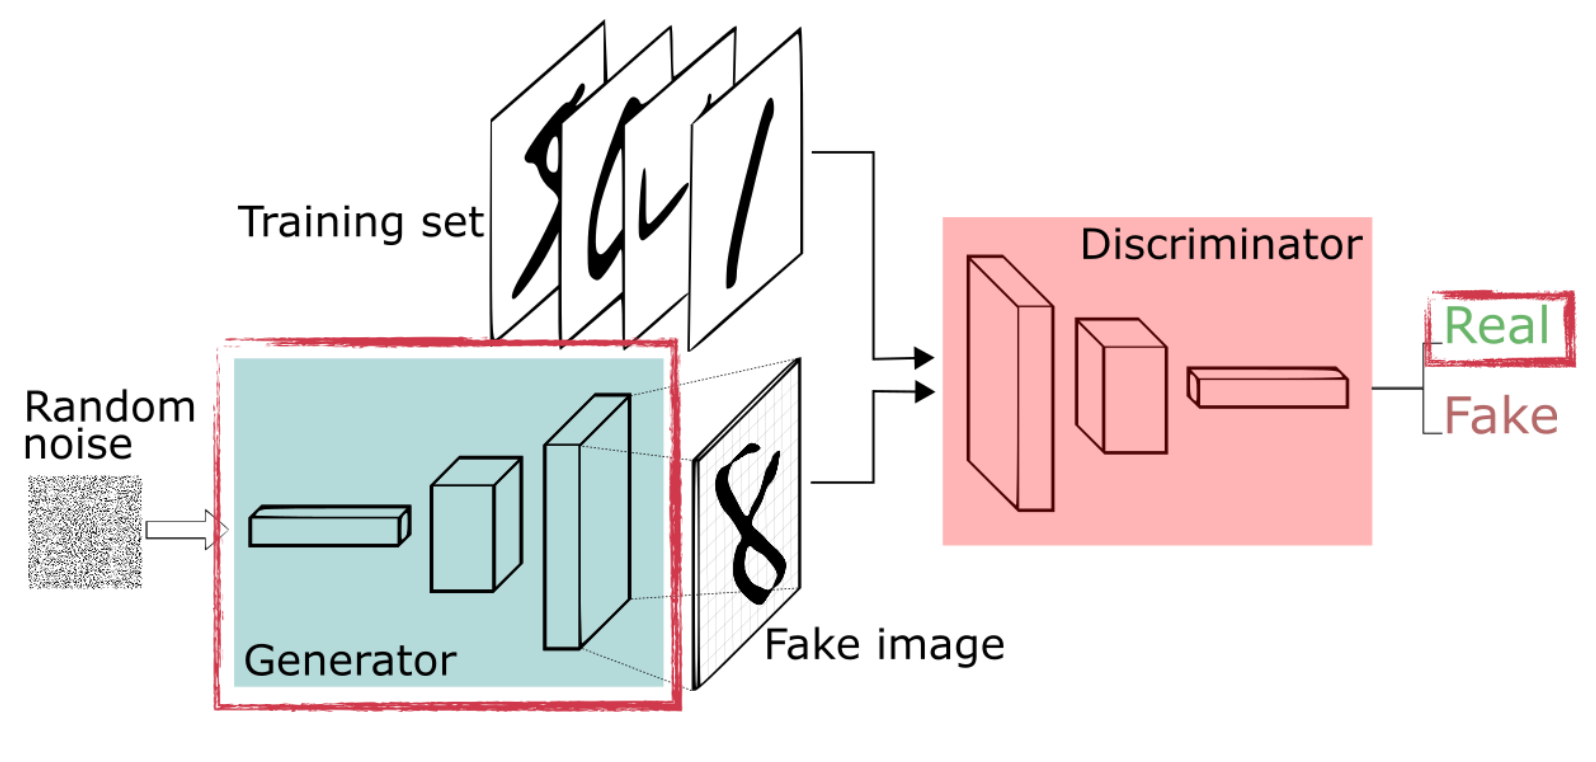
\includegraphics[width=1\textwidth]{figures/c4_divergent/diagrams/normal-gan-training.png}}
  \hfill
  \subfloat[]{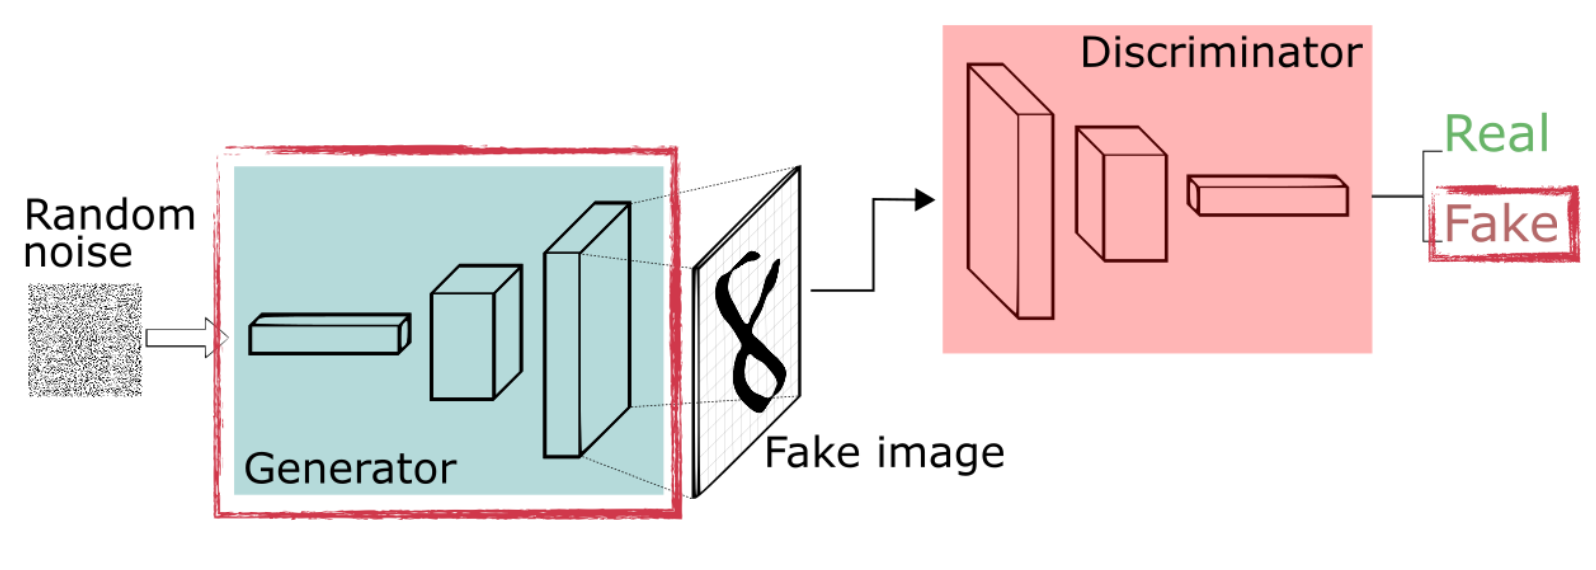
\includegraphics[width=1\textwidth]{figures/c4_divergent/diagrams/inverted-gan-loss.png}}
  \caption[Adversarial and inverted adversarial loss diagram]{Diagrams showing the standard GAN training regime with the loss that the generator is optimised towards (a), and the inverted adversarial loss fine-tuning procedure with the alternative loss for the generator network (b).}
  \label{fig:c4:gan-diagrams}
\end{figure}

In a second set of experiments this loss is modified to take the natural logarithm of the modified GAN loss:

\begin{equation} 
  \max_{G}\log(\mathbb{E}_{x\sim p_{\text{data}}(x)}[\log{D(x)}] +  \mathbb{E}_{z\sim p_{\text{z}}(z)}[1 - \log{D(G(z))}])
  \label{eq:ln-inverted-adv-loss}
  \end{equation}

The results from this operation can be seen in \S \ref{c4:sec:log-loss}.

For each model checkpoint (256,512 \& 1024) and for each loss function (inverse adversarial, log-inverse adversarial) three fine-tuning runs were performed with different parameters used for the batch size during training: 2, 4 \& 8.
Experimenting with different conditions for batch size was done in order to determine if this would have an impact on the generated results, as it is widely assumed that increasing the batch size improves visual fidelity in the standard GAN training regime. Adjusting the batch size may also impact the diversity of generated outputs, something that I observed in the experiments in Chapter \ref{ch:unstable_eq}.

For the standard inverted adversarial loss function (Eq. \ref{eq:inverted-adv-loss}), the fine-tuning procedure is run for 1000 iterations.
For the natural logarithm of the inverted adversarial loss function (Eq. \ref{eq:ln-inverted-adv-loss}), fine-tuning is run for 10000 iterations.
The reason for the difference in iteration count is that the log-loss is less aggressive and therefore the fine-tuning procedure does not collapse as quickly as the standard loss \ref{eq:inverted-adv-loss}.

\section{Results}
\label{c4:sec:results}

This section shows the results of the fine-tuning training procedure. 
It is divided into two sub-sections the first (\S \ref{c4:sec:og-loss}) shows the results of the standard inverted adversarial loss (Eq. \ref{eq:inverted-adv-loss}), the second (\S \ref{c4:sec:log-loss}) shows the results for the natural logarithm of the inverted adversarial loss (Eq. \ref{eq:ln-inverted-adv-loss}).

\subsection{Inverted Adversarial Loss}
\FloatBarrier

This section shows the results of the standard inverted adversarial loss (Eq. \ref{eq:inverted-adv-loss}). For all of these experiments with this loss function the fine-tuning procedure was performed for 1000 iterations.
Figures \ref{fig:c4:256-OG-samples} \& \ref{fig:c4:256-OG-losses} show the generated samples and losses during fine-tuning for the 256x256 checkpoint.
Figures \ref{fig:c4:512-OG-samples} \& \ref{fig:c4:512-OG-losses} show the generated samples and losses during fine-tuning for the 512x512 checkpoint.
Figures \ref{fig:c4:1024-OG-samples} \& \ref{fig:c4:1024-OG-losses} show the generated samples and losses during fine-tuning for the 1024x1024 checkpoint.

\label{c4:sec:og-loss}
\begin{figure}[!htbp]
    \centering
    \subfloat[]{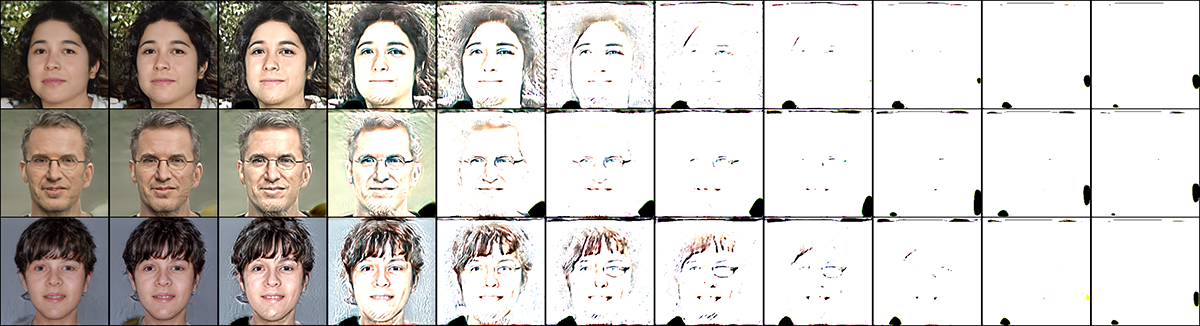
\includegraphics[width=1\textwidth]{figures/c4_divergent/gen-plots/OG/256/256-OG-2-Images-1000.png}}
    \hfill
    \subfloat[]{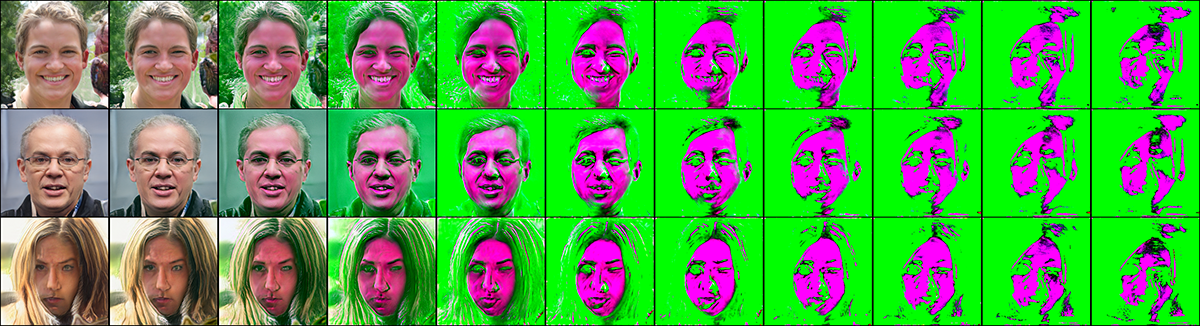
\includegraphics[width=1\textwidth]{figures/c4_divergent/gen-plots/OG/256/256-OG-4-Images-1000.png}}
    \hfill
    \subfloat[]{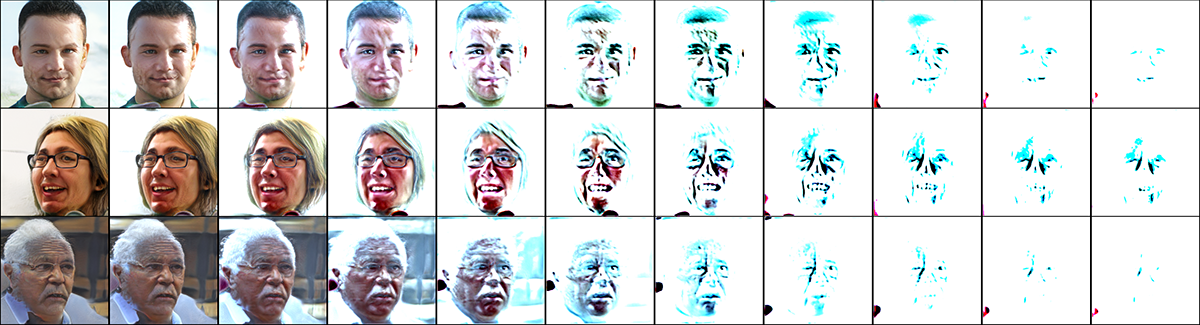
\includegraphics[width=1\textwidth]{figures/c4_divergent/gen-plots/OG/256/256-OG-8-Images-1000.png}}
    \caption[Samples of generations during the fine-tuning procedure for 256x256 StyleGAN model with the inverted adversarial loss function]{Samples of generations during the fine-tuning procedure for 256x256 StyleGAN model with the inverted adversarial loss function, at increments of 100, between training step 0-10000. (a) Results with batch size 2. (b) Results with batch size 4. (c) Results with batch size 8.}
    \label{fig:c4:256-OG-samples}
  \end{figure}

  \begin{figure}[!htbp]
    \centering
    \subfloat[]{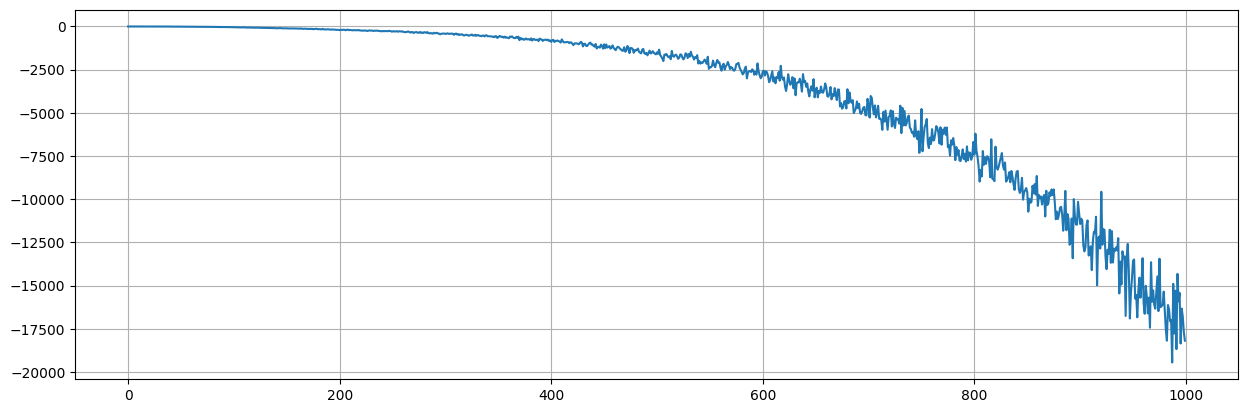
\includegraphics[width=0.8\textwidth]{figures/c4_divergent/loss-plots/OG/256/256-B2.png}}
    \hfill
    \subfloat[]{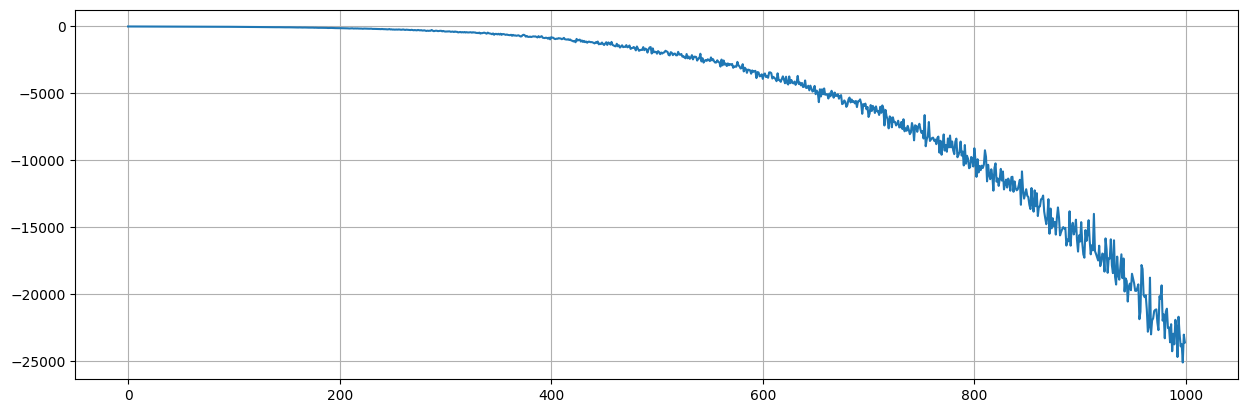
\includegraphics[width=0.8\textwidth]{figures/c4_divergent/loss-plots/OG/256/256-B4.png}}
    \hfill
    \subfloat[]{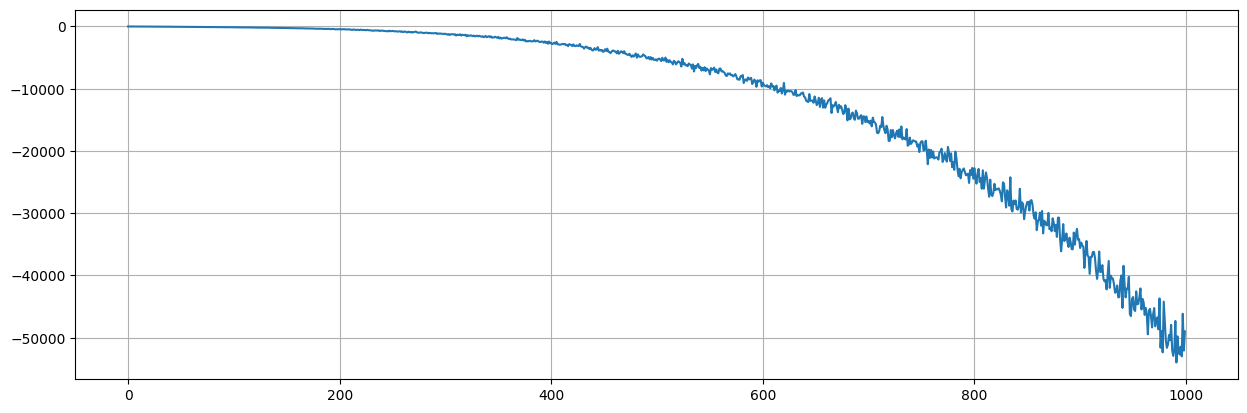
\includegraphics[width=0.8\textwidth]{figures/c4_divergent/loss-plots/OG/256/256-B8.png}}
    \caption[Loss plots for the fine-tuning procedure for 256x256 StyleGAN model with the inverted adversarial loss function]{Loss plots for the fine-tuning procedure for 256x256 StyleGAN model with the inverted adversarial loss function. (a) Results with batch size 2. (b) Results with batch size 4. (c) Results with batch size 8.}
    \label{fig:c4:256-OG-losses}
  \end{figure}

  \begin{figure}[!htbp]
    \centering
    \subfloat[]{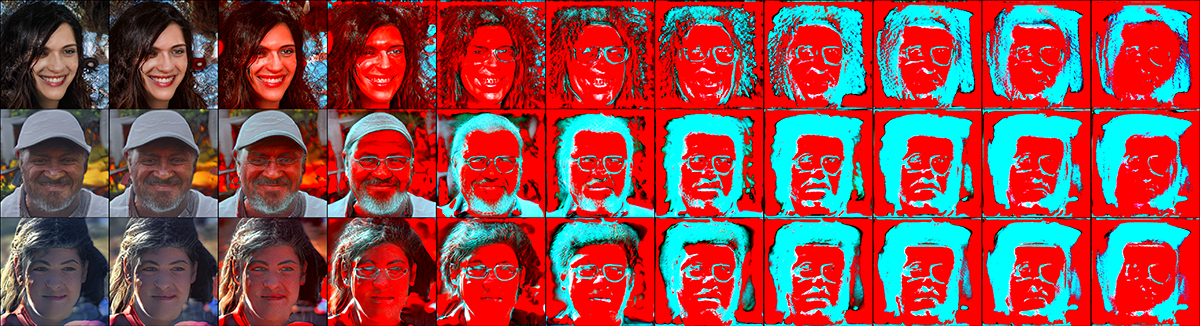
\includegraphics[width=1\textwidth]{figures/c4_divergent/gen-plots/OG/512/512-OG-2-Images-1000.png}}
    \hfill
    \subfloat[]{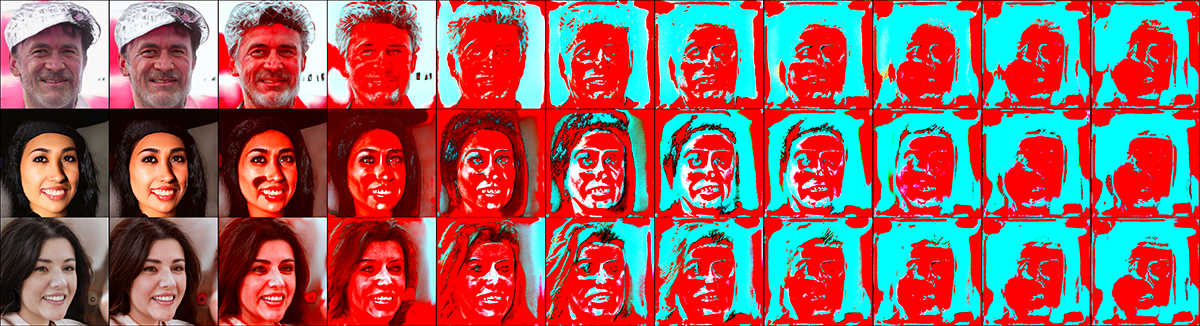
\includegraphics[width=1\textwidth]{figures/c4_divergent/gen-plots/OG/512/512-OG-4-Images-1000.png}}
    \hfill
    \subfloat[]{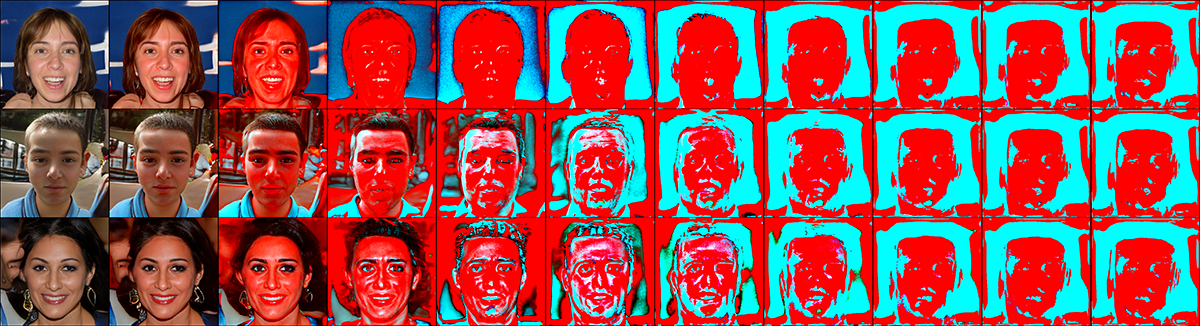
\includegraphics[width=1\textwidth]{figures/c4_divergent/gen-plots/OG/512/512-OG-8-Images-1000.png}}
    \caption[Samples of generations during the fine-tuning procedure for 512x512 StyleGAN model with the inverted adversarial loss function]{Samples of generations during the fine-tuning procedure for 512x512 StyleGAN model with the inverted adversarial loss function, at increments of 100, between training step 0-1000. (a) Results with batch size 2. (b) Results with batch size 4. (c) Results with batch size 8.}
    \label{fig:c4:512-OG-samples}
  \end{figure}

  \begin{figure}[!htbp]
    \centering
    \subfloat[]{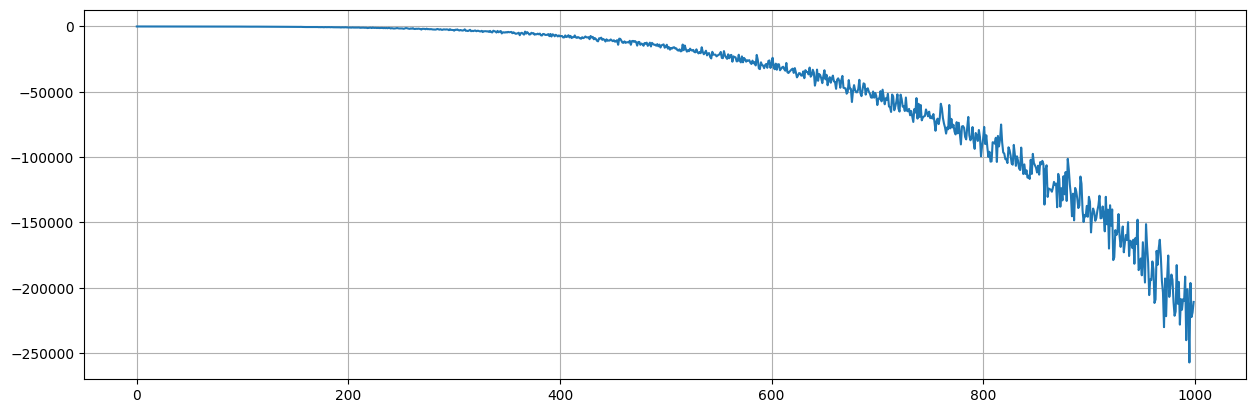
\includegraphics[width=0.8\textwidth]{figures/c4_divergent/loss-plots/OG/512/512-B2.png}}
    \hfill
    \subfloat[]{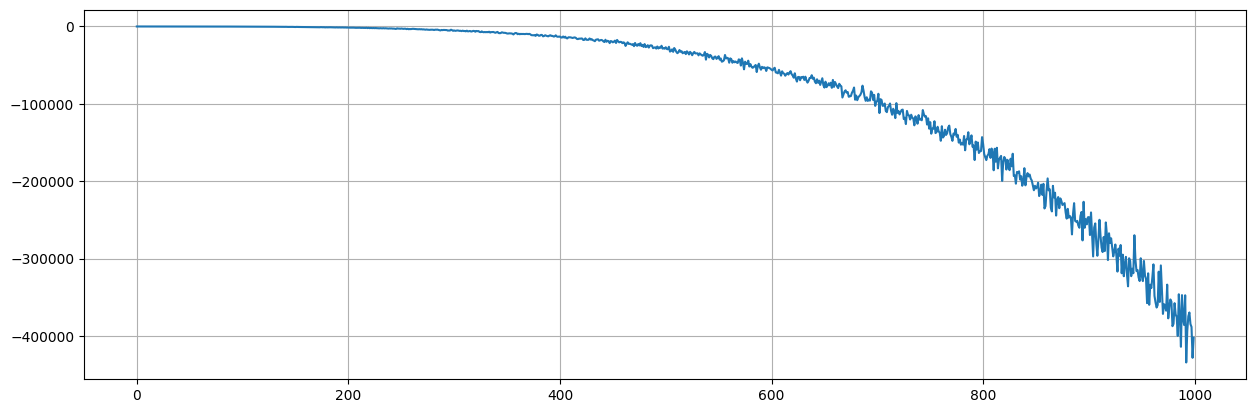
\includegraphics[width=0.8\textwidth]{figures/c4_divergent/loss-plots/OG/512/512-B4.png}}
    \hfill
    \subfloat[]{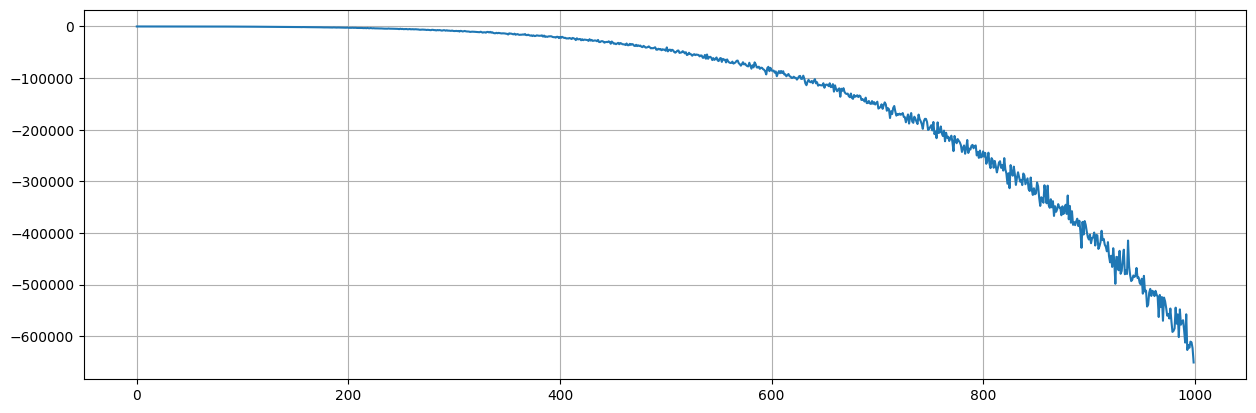
\includegraphics[width=0.8\textwidth]{figures/c4_divergent/loss-plots/OG/512/512-B8.png}}
    \caption[Loss plots for the fine-tuning procedure for 512x512 StyleGAN model with the inverted adversarial loss function]{Loss plots for the fine-tuning procedure for 512x512 StyleGAN model with the inverted adversarial loss function. (a) Results with batch size 2. (b) Results with batch size 4. (c) Results with batch size 8.}
    \label{fig:c4:512-OG-losses}
  \end{figure}

  \begin{figure}[!htbp]
    \centering
    \subfloat[]{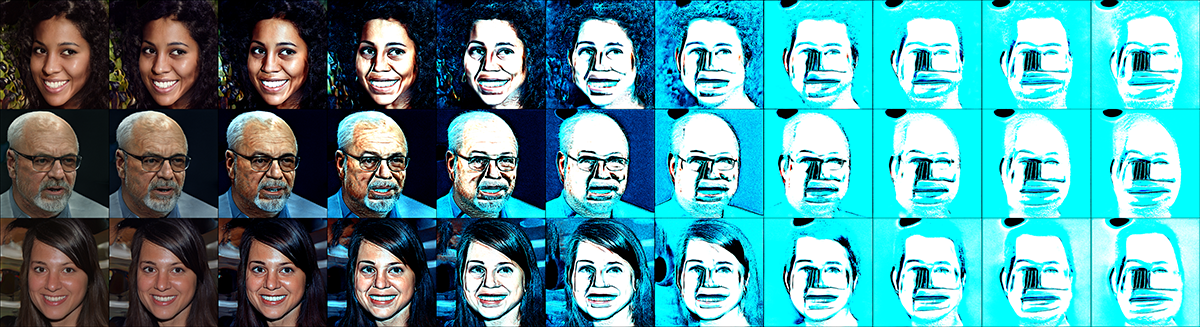
\includegraphics[width=1\textwidth]{figures/c4_divergent/gen-plots/OG/1024/1024-OG-2-Images-1000.png}}
    \hfill
    \subfloat[]{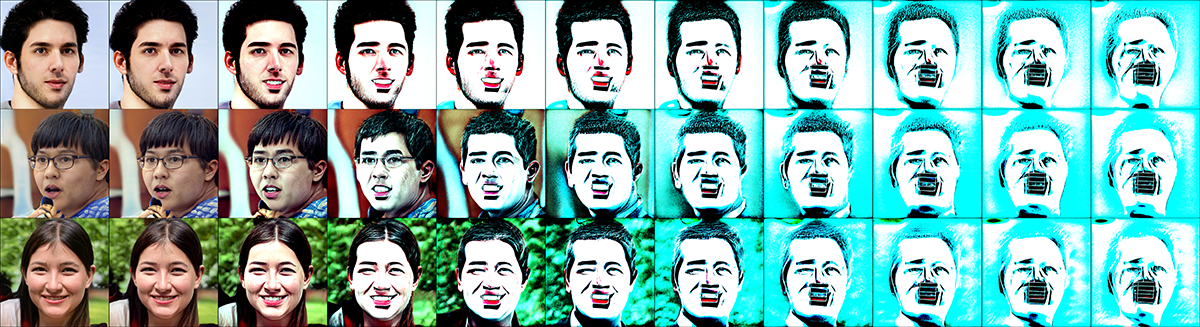
\includegraphics[width=1\textwidth]{figures/c4_divergent/gen-plots/OG/1024/1024-OG-4-Images-1000.png}}
    \hfill
    \subfloat[]{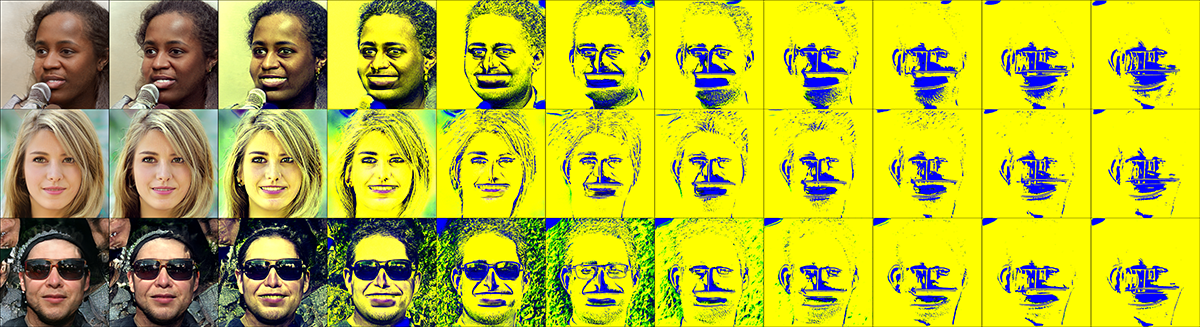
\includegraphics[width=1\textwidth]{figures/c4_divergent/gen-plots/OG/1024/1024-OG-8-Images-1000.png}}
    \caption[Samples of generations during the fine-tuning procedure for 1024x1024 StyleGAN model with the inverted adversarial loss function]{Samples of generations during the fine-tuning procedure for 1024x1024 StyleGAN model with the inverted adversarial loss function, at increments of 100, between training step 0-1000. (a) Results with batch size 2. (b) Results with batch size 4. (c) Results with batch size 8.}
    \label{fig:c4:1024-OG-samples}
  \end{figure}

  \begin{figure}[!htbp]
    \centering
    \subfloat[]{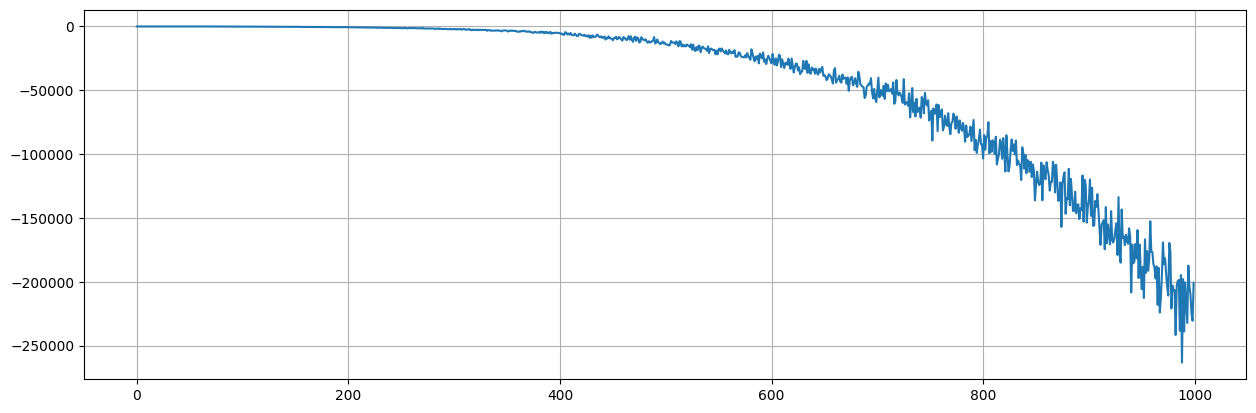
\includegraphics[width=0.8\textwidth]{figures/c4_divergent/loss-plots/OG/1024/1024-B2.png}}
    \hfill
    \subfloat[]{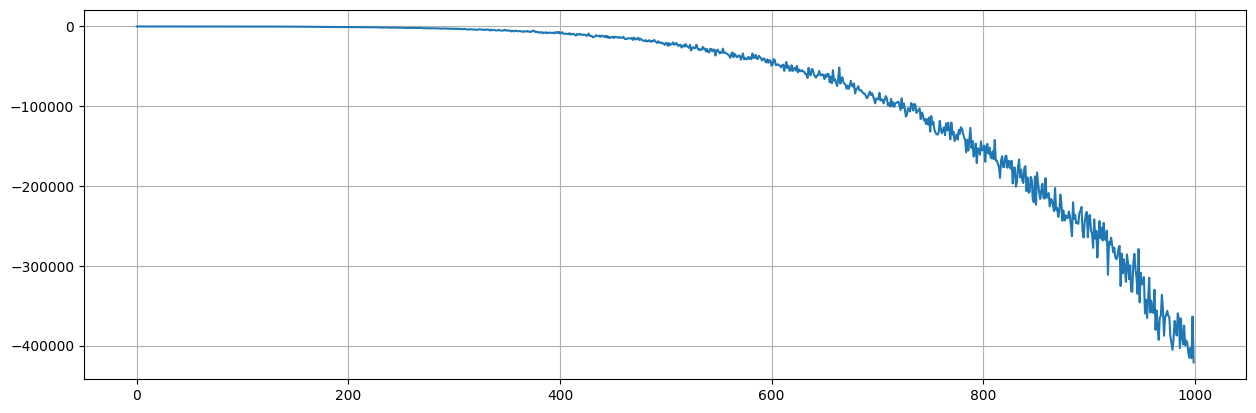
\includegraphics[width=0.8\textwidth]{figures/c4_divergent/loss-plots/OG/1024/1024-B4.png}}
    \hfill
    \subfloat[]{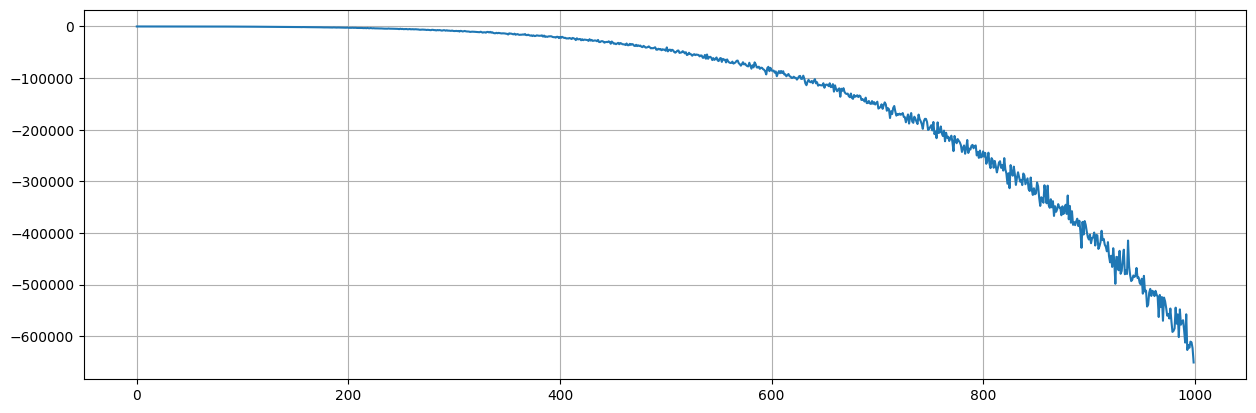
\includegraphics[width=0.8\textwidth]{figures/c4_divergent/loss-plots/OG/1024/1024-B8.png}}
    \caption[Loss plots for the fine-tuning procedure for 1024x1024 StyleGAN model with the inverted adversarial loss function]{Loss plots for the fine-tuning procedure for 1024x1024 StyleGAN model with the inverted adversarial loss function. (a) Results with batch size 2. (b) Results with batch size 4. (c) Results with batch size 8.}
    \label{fig:c4:1024-OG-losses}
  \end{figure}

\FloatBarrier

\subsection{Natural Logarithm of Inverted Adversarial Loss}
\label{c4:sec:log-loss}

This section shows the results of the standard inverted adversarial loss (Eq. \ref{eq:ln-inverted-adv-loss}). For all of these experiments with this loss function the fine-tuning procedure was performed for 10000 iterations.
Figures \ref{fig:c4:256-LOG-samples} \& \ref{fig:c4:256-LOG-losses} show the generated samples and losses during fine-tuning for the 256x256 checkpoint.
Figures \ref{fig:c4:512-LOG-samples} \& \ref{fig:c4:512-LOG-losses} show the generated samples and losses during fine-tuning for the 512x512 checkpoint.
Figures \ref{fig:c4:1024-LOG-samples} \& \ref{fig:c4:1024-LOG-losses} show the generated samples and losses during fine-tuning for the 1024x1024 checkpoint.

\begin{figure}[!htbp]
    \centering
    \subfloat[]{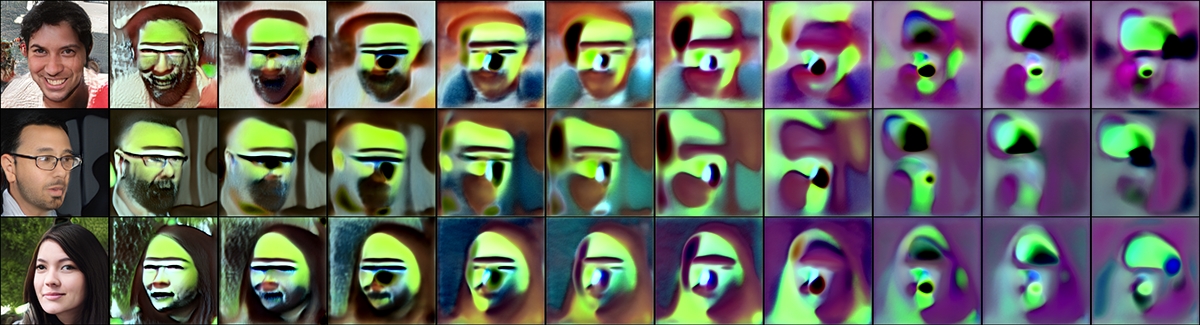
\includegraphics[width=1\textwidth]{figures/c4_divergent/gen-plots/LOG/256/256-LOG-2-Images-10000.png}}
    \hfill
    \subfloat[]{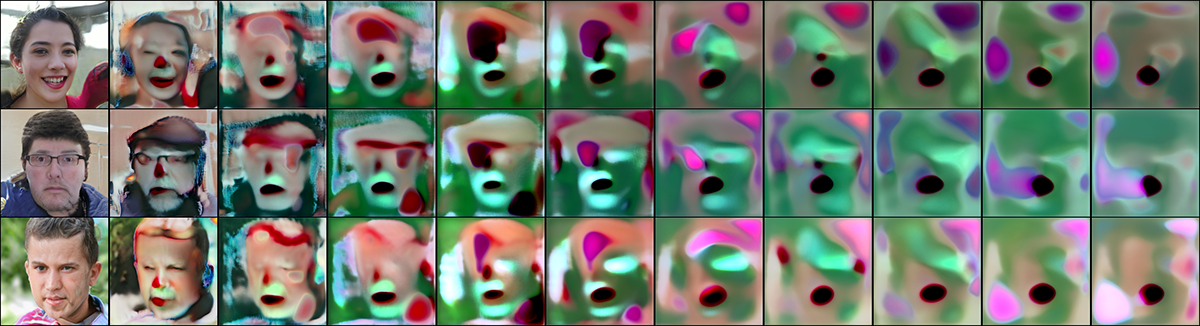
\includegraphics[width=1\textwidth]{figures/c4_divergent/gen-plots/LOG/256/256-LOG-4-Images-10000.png}}
    \hfill
    \subfloat[]{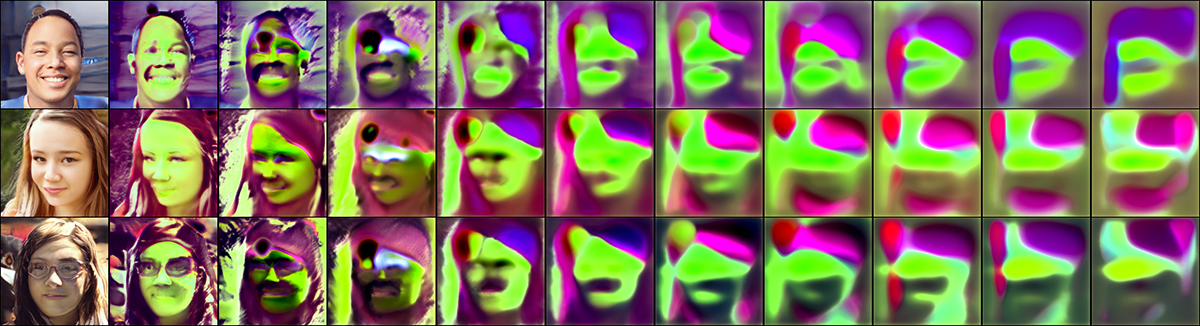
\includegraphics[width=1\textwidth]{figures/c4_divergent/gen-plots/LOG/256/256-LOG-8-Images-10000.png}}
    \caption[Samples of generations during the fine-tuning procedure for 256x256 StyleGAN model with the natural logarithm of the inverted adversarial loss function]{Samples of generations during the fine-tuning procedure for 256x256 StyleGAN model with the natural logarithm of the inverted adversarial loss function, at increments of 1000, between training step 0-10000. (a) Results with batch size 2. (b) Results with batch size 4. (c) Results with batch size 8.}
    \label{fig:c4:256-LOG-samples}
  \end{figure}

  \begin{figure}[!htbp]
    \centering
    \subfloat[]{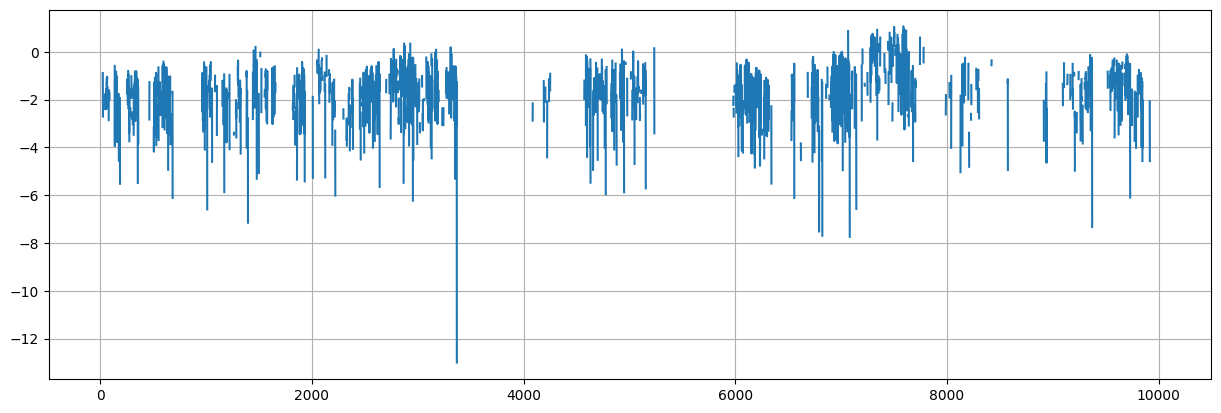
\includegraphics[width=0.8\textwidth]{figures/c4_divergent/loss-plots/LOG/256/256-B2.png}}
    \hfill
    \subfloat[]{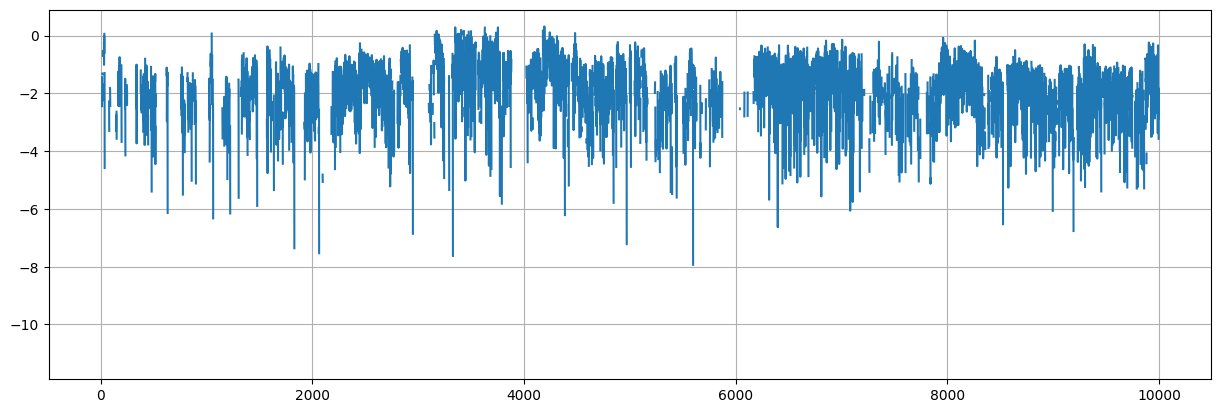
\includegraphics[width=0.8\textwidth]{figures/c4_divergent/loss-plots/LOG/256/256-B4.png}}
    \hfill
    \subfloat[]{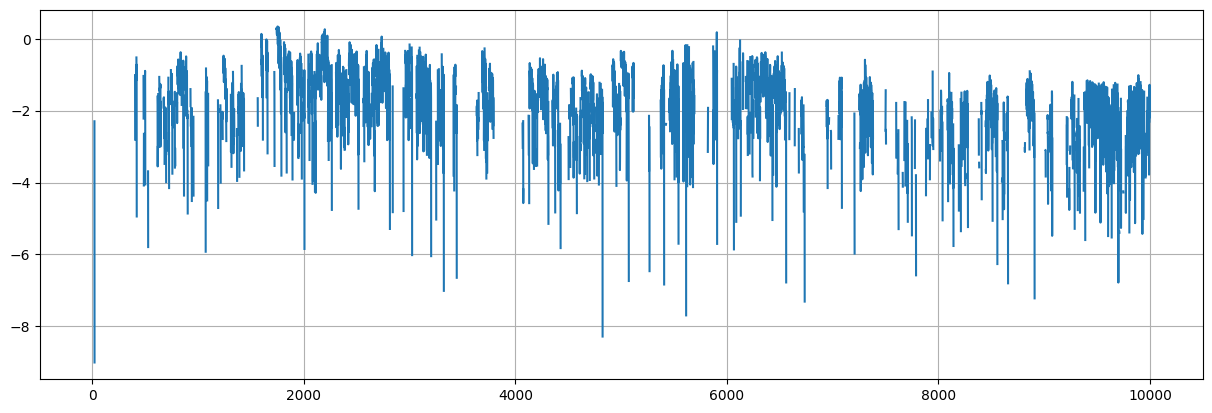
\includegraphics[width=0.8\textwidth]{figures/c4_divergent/loss-plots/LOG/256/256-B8.png}}
    \caption[Loss plots for fine-tuning procedure for 256x256 StyleGAN model with the natural logarithm of the inverted adversarial loss function]{Loss plots for fine-tuning procedure for 256x256 StyleGAN model with the natural logarithm of the inverted adversarial loss function. (a) Results with batch size 2. (b) Results with batch size 4. (c) Results with batch size 8. Note: gaps in the plot are where the loss was undefined from taking the log of a negative number.}
    \label{fig:c4:256-LOG-losses}
  \end{figure}

  \begin{figure}[!htbp]
    \centering
    \subfloat[]{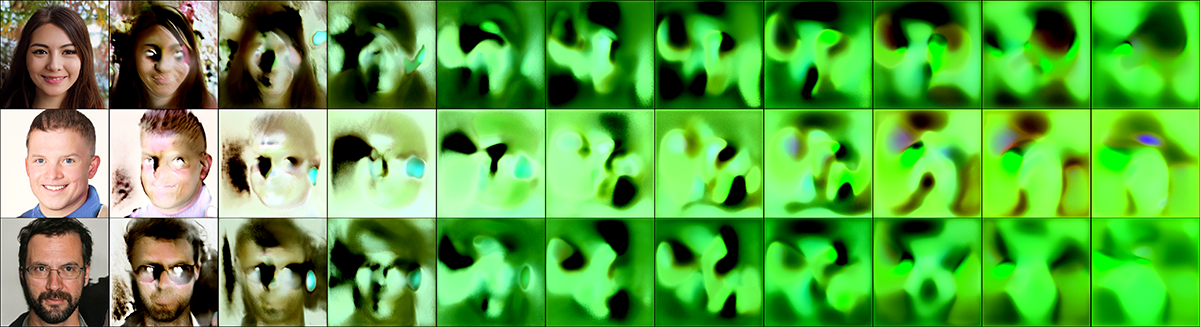
\includegraphics[width=1\textwidth]{figures/c4_divergent/gen-plots/LOG/512/512-LOG-2-Images-10000.png}}
    \hfill
    \subfloat[]{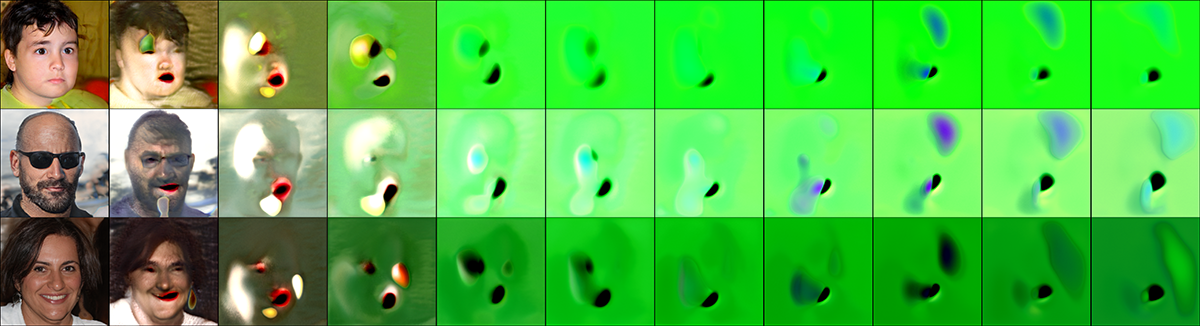
\includegraphics[width=1\textwidth]{figures/c4_divergent/gen-plots/LOG/512/512-LOG-4-Images-10000.png}}
    \hfill
    \subfloat[]{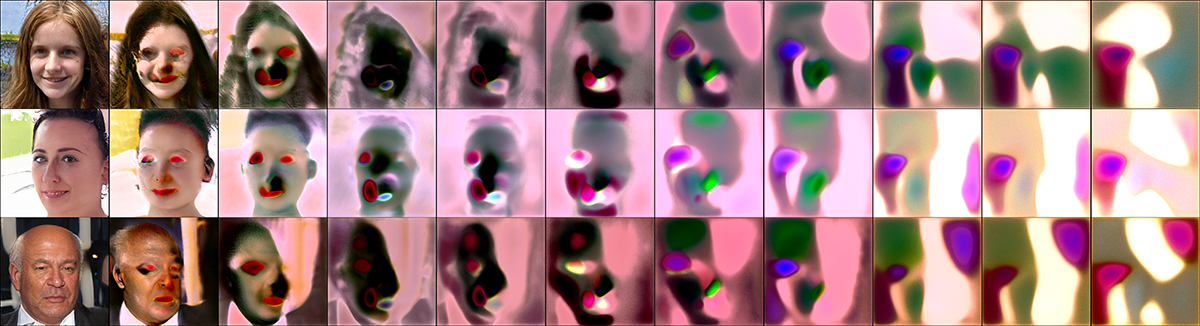
\includegraphics[width=1\textwidth]{figures/c4_divergent/gen-plots/LOG/512/512-LOG-8-Images-10000.png}}
    \caption[Samples of generations during the fine-tuning procedure for 512x512 StyleGAN model with the natural logarithm of the inverted adversarial loss function]{Samples of generations during the fine-tuning procedure for 512x512 StyleGAN model with the natural logarithm of the inverted adversarial loss function, at increments of 1000, between training step 0-10000. (a) Results with batch size 2. (b) Results with batch size 4. (c) Results with batch size 8.}
    \label{fig:c4:512-LOG-samples}
  \end{figure}

  \begin{figure}[!htbp]
    \centering
    \subfloat[]{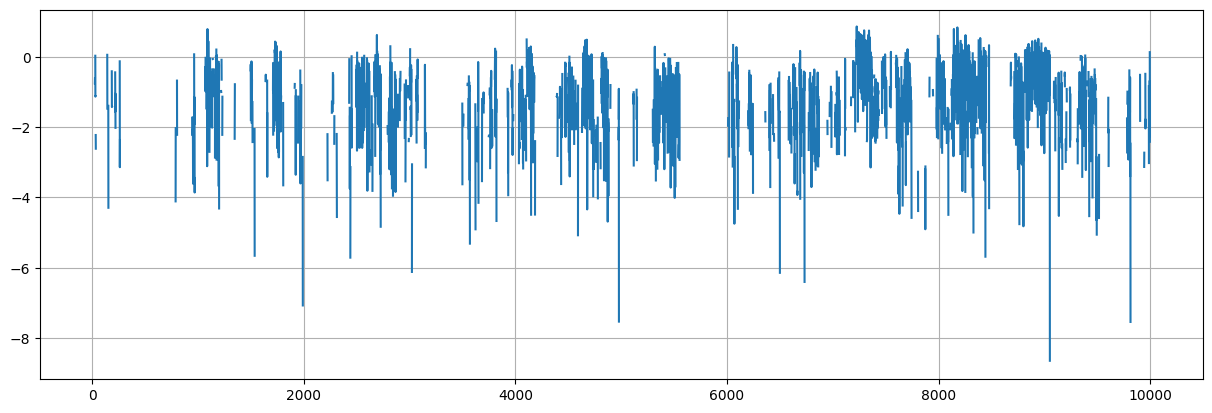
\includegraphics[width=0.8\textwidth]{figures/c4_divergent/loss-plots/LOG/512/512-B2.png}}
    \hfill
    \subfloat[]{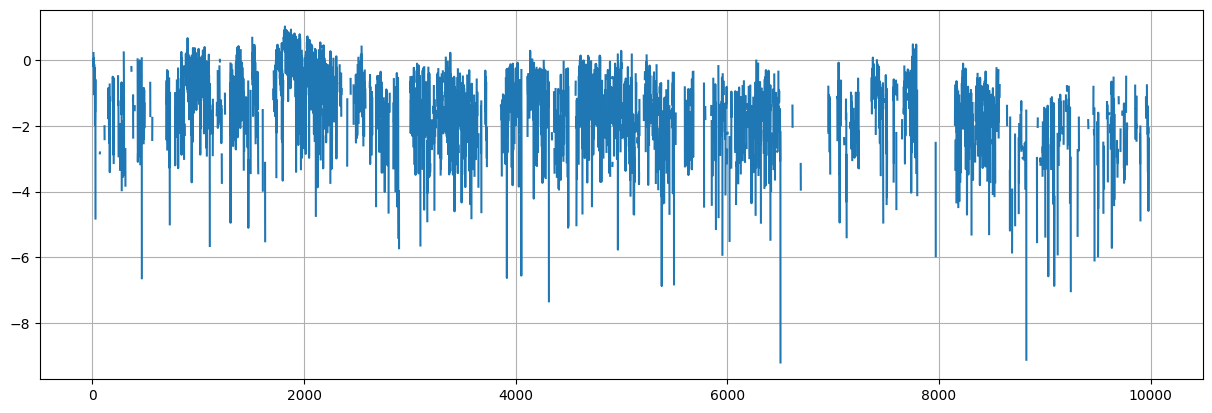
\includegraphics[width=0.8\textwidth]{figures/c4_divergent/loss-plots/LOG/512/512-B4.png}}
    \hfill
    \subfloat[]{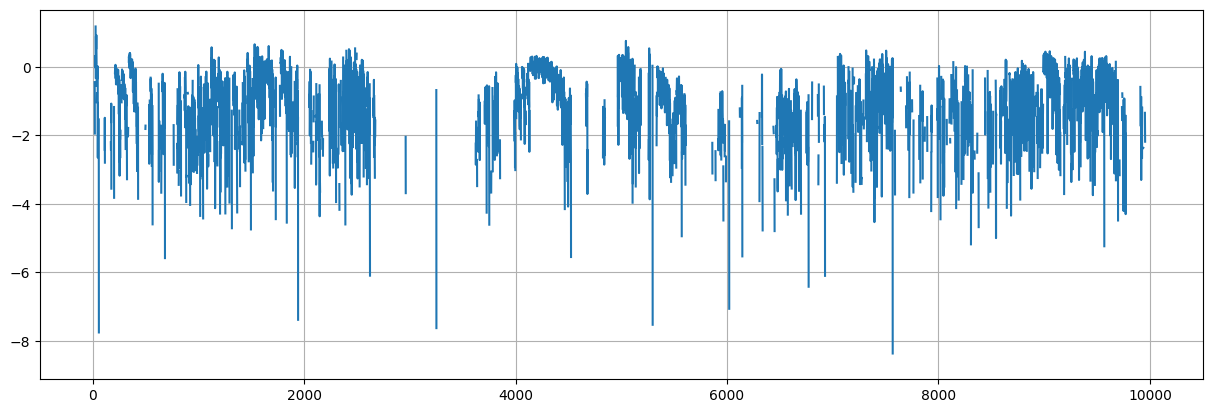
\includegraphics[width=0.8\textwidth]{figures/c4_divergent/loss-plots/LOG/512/512-B8.png}}
    \caption[Loss plots for fine-tuning procedure for 512x512 StyleGAN model with the natural logarithm of the inverted adversarial loss function]{Loss plots for fine-tuning procedure for 512x512 StyleGAN model with the natural logarithm of the inverted adversarial loss function. (a) Results with batch size 2. (b) Results with batch size 4. (c) Results with batch size 8. Note: gaps in the plot are where the loss was undefined from taking the log of a negative number.}
    \label{fig:c4:512-LOG-losses}
  \end{figure}

  \begin{figure}[!htbp]
    \centering
    \subfloat[]{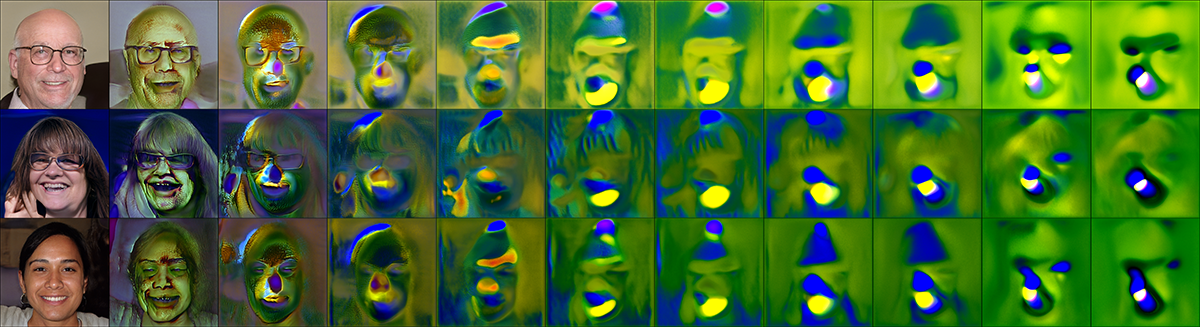
\includegraphics[width=1\textwidth]{figures/c4_divergent/gen-plots/LOG/1024/1024-LOG-2-Images-10000.png}}
    \hfill
    \subfloat[]{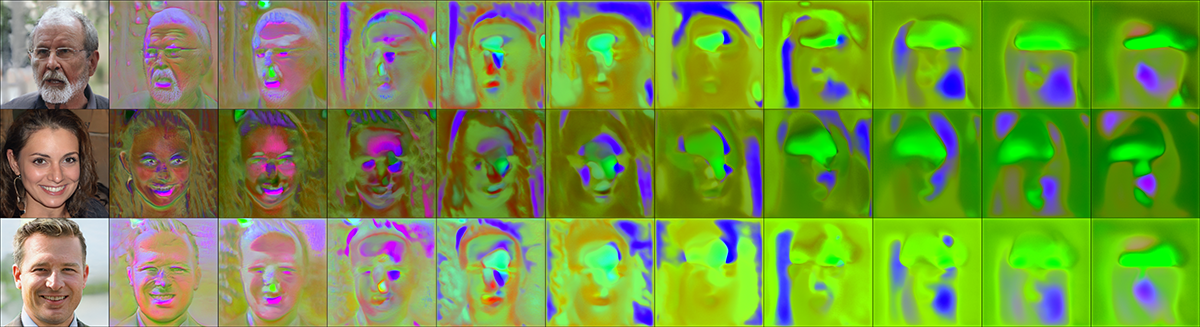
\includegraphics[width=1\textwidth]{figures/c4_divergent/gen-plots/LOG/1024/1024-LOG-4-Images-10000.png}}
    \hfill
    \subfloat[]{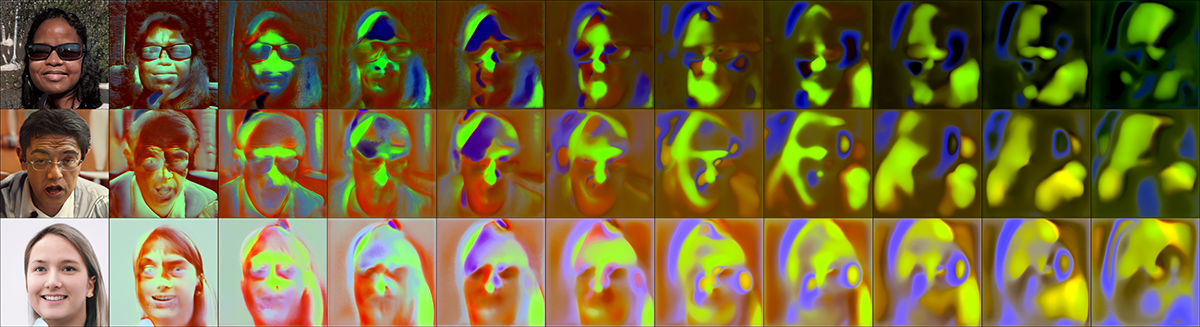
\includegraphics[width=1\textwidth]{figures/c4_divergent/gen-plots/LOG/1024/1024-LOG-8-Images-10000.png}}
    \caption[Samples of generations during the fine-tuning procedure for 1024x1024 StyleGAN model with the natural logarithm of the inverted adversarial loss function]{Samples of generations during the fine-tuning procedure for 1024x1024 StyleGAN model with the natural logarithm of the inverted adversarial loss function, at increments of 1000, between training step 0-10000. (a) Results with batch size 2. (b) Results with batch size 4. (c) Results with batch size 8.}
    \label{fig:c4:1024-LOG-samples}
  \end{figure}

  \begin{figure}[!htbp]
    \centering
    \subfloat[]{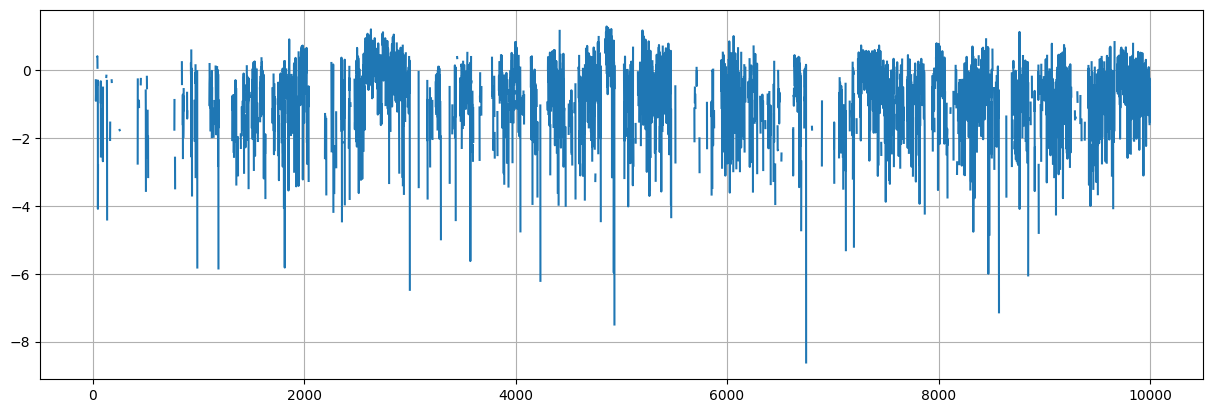
\includegraphics[width=0.8\textwidth]{figures/c4_divergent/loss-plots/LOG/1024/1024-B2.png}}
    \hfill
    \subfloat[]{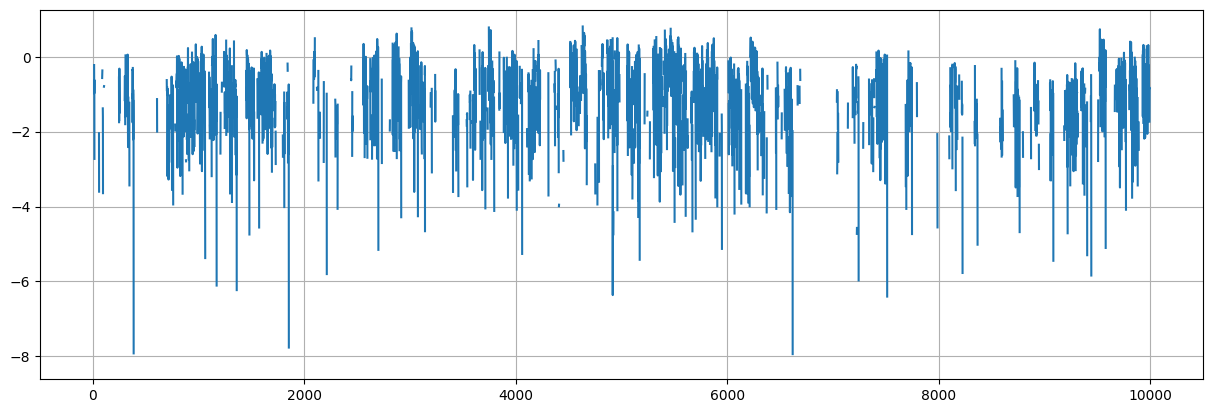
\includegraphics[width=0.8\textwidth]{figures/c4_divergent/loss-plots/LOG/1024/1024-B4.png}}
    \hfill
    \subfloat[]{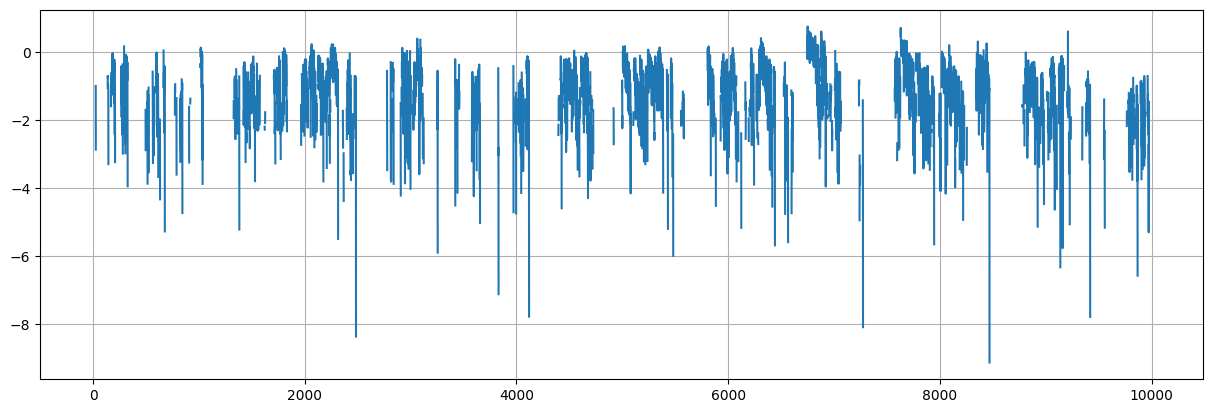
\includegraphics[width=0.8\textwidth]{figures/c4_divergent/loss-plots/LOG/1024/1024-B8.png}}
    \caption[Loss plots for fine-tuning procedure for 1024x1024 StyleGAN model with the natural logarithm of the inverted adversarial loss function]{Loss plots for fine-tuning procedure for 1024x1024 StyleGAN model with the natural logarithm of the inverted adversarial loss function. (a) Results with batch size 2. (b) Results with batch size 4. (c) Results with batch size 8. Note: gaps in the plot are where the loss was undefined from taking the log of a negative number.} 
    \label{fig:c4:1024-LOG-losses}
  \end{figure}

\FloatBarrier

\section{Discussion}

The results presented here demonstrate an efficient method of divergent fine-tuning, away from the likelihood of the original training data. 
The results from the first loss function show a method that quickly optimises towards a fixed representation of `unlikelihood'.
Of course, this representation of unlikelihood is contingent on the particular state of the two models (generator and discriminator) that is then fixed when the model checkpoints are saved during the training process.
GAN, unlike many other training regimes for generative models,  does not converge to a fixed point in the optimisation process.
Instead, they act as a dynamic system, with no target end state. 
The optimisation problem in adversarial approaches is circular \citep{nagarajan2017gradient}. 
The generator and discriminator will endlessly be playing this game of forger/detective. 
The discriminator endlessly picks up on new minuscule flaws in the generator output, and the generator in turn responds, in an endless adversarial game.
Therefore, for each different saved checkpoint of the discriminator, different attributes that define unlikelihood are optimised towards.
It is clear in the visual results of the different models using the first loss function ( Eq. \ref{eq:inverted-adv-loss}; Figures \ref{fig:c4:256-OG-samples},\ref{fig:c4:512-OG-samples} \& \ref{fig:c4:1024-OG-samples}), that there are clear and specific things being optimised toward.
This shows clearly that this is ever-changing in the training process.

Whilst the results for the standard loss show that there is a generally coherent fixed point of optimisation for each of the model snapshots, there are minor visual differences in each of the different training runs.
Whilst it would be easy to attribute this solely to the change in the batch size parameter, I suspect that the sampling regime is also a contingent part of the visual differences between the different training runs.
Input latents for the generator are sampled randomly, and this random sampling and the sequence in which random latents are sampled may be just as important in determining the direction for optimisation and the final visual results, as much as the batch size used in each of these training runs. 

For the second loss function \ref{eq:ln-inverted-adv-loss}, which uses the natural log of the inverse adversarial loss, there is clearly much less of a fixed point to which the optimiser is moving. 
Whilst there are similarities in all of these final results (abstract shapes with generally consistent colours), there is clearly not one fixed point here that is being optimised for each of the model checkpoints.
By taking the log of the loss, this appears to keep the range of the loss function within a much more constrained range.
The losses in the first experiment, quickly explode into very high ranges (exceeding -600000 in some cases), which is due to the feedback loop of reinforcing changes, where any change the the parameters of the generator further increases the loss.
By taking the log of the loss this feedback loop is nullified. 
There are likely two things at play here, in log space the exponential feedback loop is far less aggressive. 
As these loss scores also tend towards negative numbers, thus when we take the log of this loss, these negative numbers become undefined (as taking the log of a negative number is always undefined).
As you can see in Figures \ref{fig:c4:256-LOG-losses},\ref{fig:c4:512-LOG-losses} \& \ref{fig:c4:1024-LOG-losses}, there are large gaps where there is loss in underfined .\footnote{Surprisingly, backpropagating undefined numbers does not seem to be an issue in pytorch.}
Once again this may act as a constraint that prevents the feedback loop seen in Figures \ref{fig:c4:256-OG-losses},\ref{fig:c4:512-OG-losses} \& \ref{fig:c4:1024-OG-losses} from taking hold.

The fine-tuning procedure with Eq. \ref{eq:ln-inverted-adv-loss} appears to produce a dynamic between models that is endlessly evolving. 
Figure \ref{fig:c4:100k-iterations} shows one of these training runs continued to 100,000 iterations, where it is clear that this process is continually evolving.
In a similar fashion to the work in Chapter \ref{ch:unstable_eq} this is an endless and undefined goal, leading to a dynamic process that continually produces ever-evolving abstract outputs.

\begin{figure}[!htbp]
  \centering
  \subfloat[]{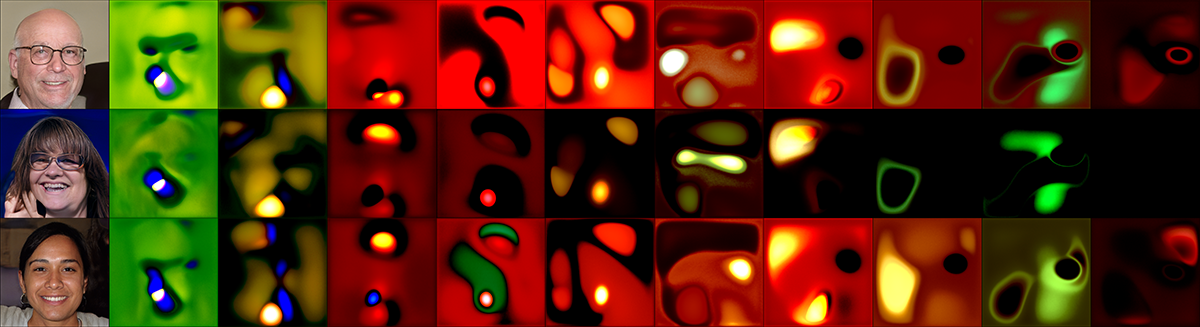
\includegraphics[width=1\textwidth]{figures/c4_divergent/discussion/log-8-100k-iterations.png}}
  \caption[100k iterations of 1024x1024 StyleGAN model with the natural logarithm of the inverted adversarial loss function]{100k iterations of 1024x1024 StyleGAN model with the natural logarithm of the inverted adversarial loss function with batch parameter 8, at increments of 10000, between training step 0-100000.}
  \label{fig:c4:100k-iterations}
\end{figure}

\subsection{Relationship to The Uncanny}

One of the observations that was made in the visual results of this process, especially in the transition stages of standard inverted loss, was the uncanny nature of the images,\footnote{
      Some of the early images I created during this process were quite disturbing  (Ref impact chapter). The first person I showed them to was my partner at the time, whose response was to the effect of: ``Well that is horrifying, please never show me those pictures again''. I later showed the results to a PhD colleague of mine, Shringi Kumari, in the Goldsmiths iGGi office, who had an equally negative reaction.} which can be seen in Figures \ref{fig:c4:uncanny-images-og} \& \ref{fig:c4:uncanny-images-log}.

\begin{figure}[!htbp]
  \vspace{-60pt}
  \centering
  \subfloat[]{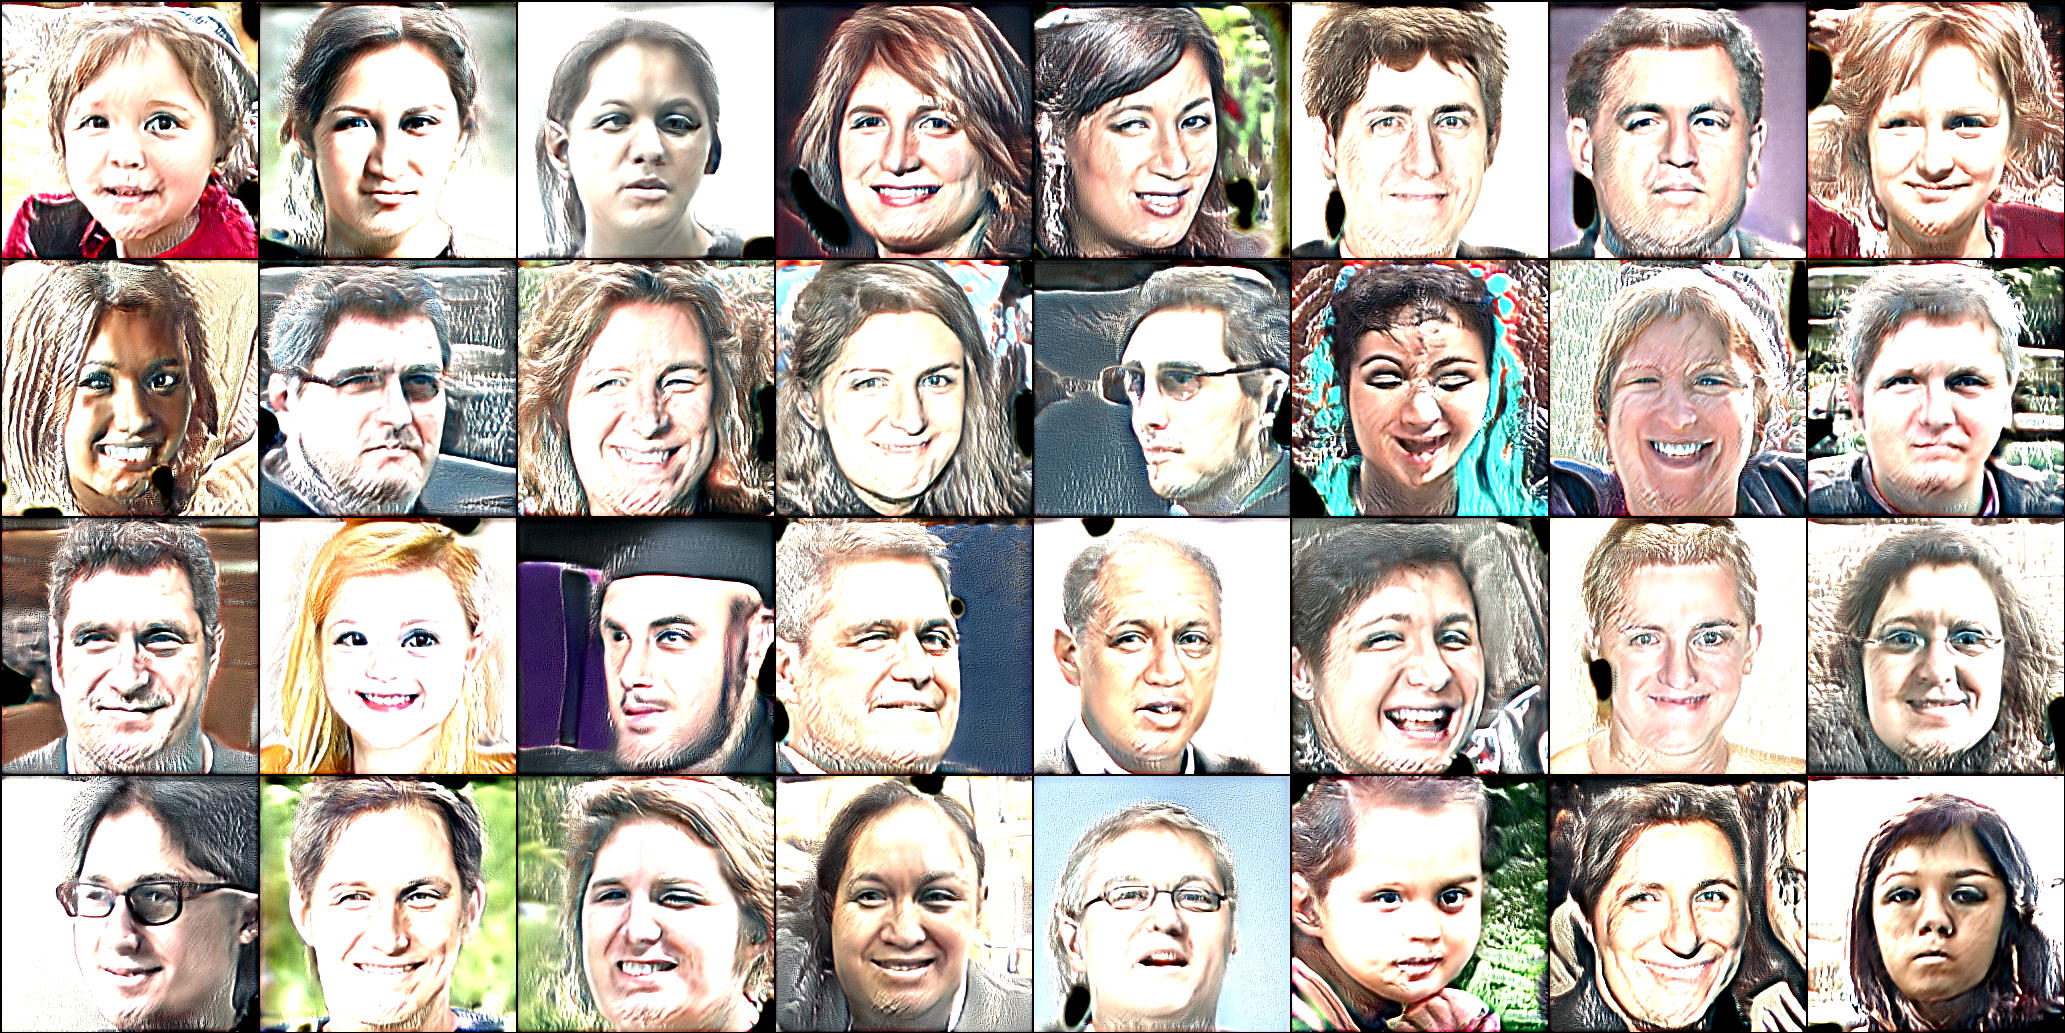
\includegraphics[width=1\textwidth]{figures/c4_divergent/discussion/grid-256-300iter.png}}
  \hfill
  \subfloat[]{\includegraphics[width=1\textwidth]{figures/c4_divergent/discussion/grid-512-300iter.png}}
  \hfill
  \subfloat[]{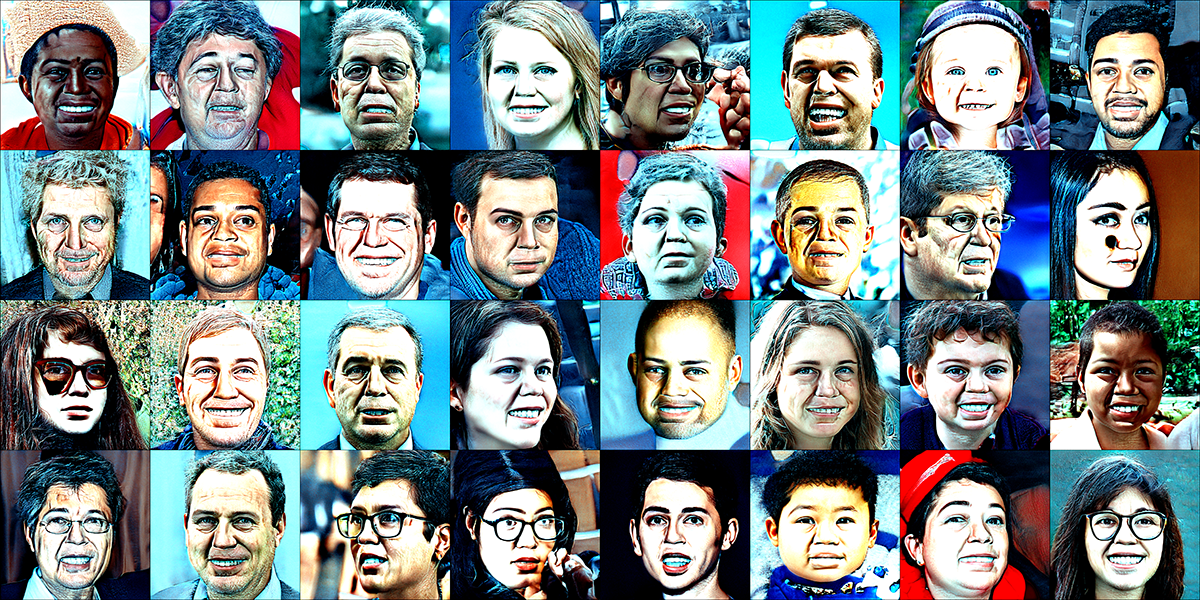
\includegraphics[width=1\textwidth]{figures/c4_divergent/discussion/grid-1024-300iter.png}}
  \caption[Uncanny images of samples from 300 iterations of fine-tuning with inverse loss]{Uncanny images of samples from 300 iterations of fine-tuning with inverse loss, using batch size of 2. (a) 256x256 model. (b) 512x512 model. (c) 1024x1024 model. }
  \label{fig:c4:uncanny-images-og}
\end{figure}

\begin{figure}[!htbp]
  \vspace{-60pt}
  \centering
  \subfloat[]{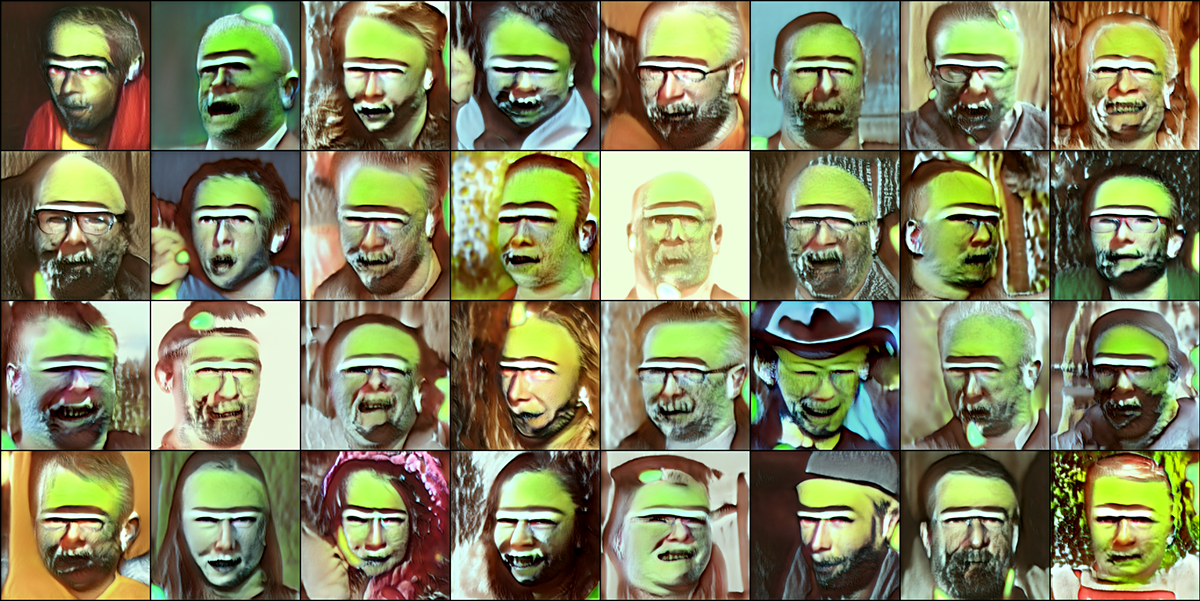
\includegraphics[width=1\textwidth]{figures/c4_divergent/discussion/grid-256-1000iter-log.png}}
  \hfill
  \subfloat[]{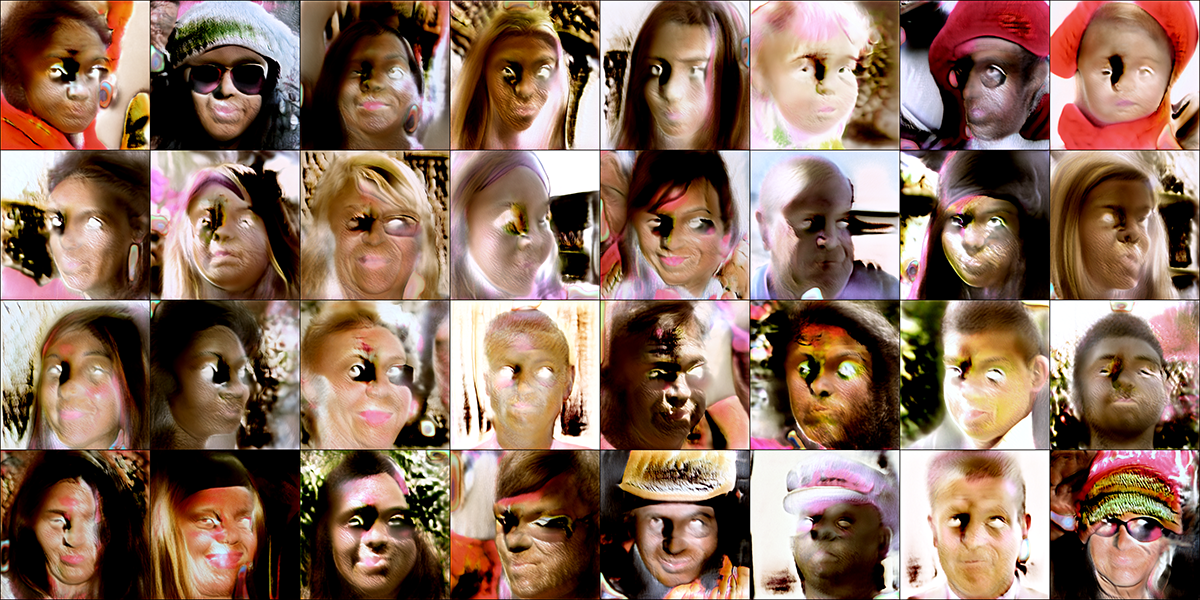
\includegraphics[width=1\textwidth]{figures/c4_divergent/discussion/grid-512-1000iter-log.png}}
  \hfill
  \subfloat[]{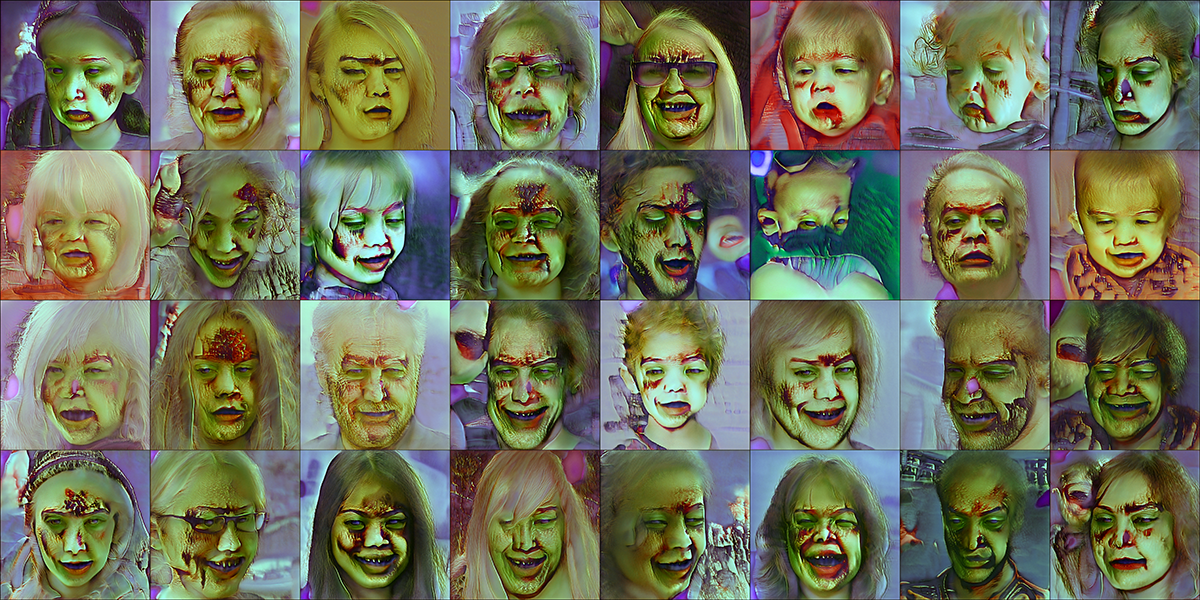
\includegraphics[width=1\textwidth]{figures/c4_divergent/discussion/grid-1024-1000iter-log.png}}
  \caption[Uncanny images of samples from 1000 iterations of fine-tuning with natural logarithm of the inverse loss]{Uncanny images of samples from 1000 iterations of fine-tuning with natural logarithm of the inverse loss, using batch size of 2. (a) 256x256 model. (b) 512x512 model. (c) 1024x1024 model. }
  \label{fig:c4:uncanny-images-log}
\end{figure}

The uncanny is a psychological or aesthetic experience that can be characterised as observing something familiar that is encountered in an unsettling way. 
Jentsch defined the uncanny as an experience that stems from uncertainty, giving an example of it as being most pronounced when there is “doubt as to whether an apparently living being is animate and, conversely, doubt as to whether a lifeless object may not in fact be animate” \citep{jentsch1997psychology}. 
This definition was later refined to argue that the uncanny occurs when something familiar is alienated when the familiar is viewed in an unexpected or unfamiliar form \citep{freud1919uncanny}.

The uncanny valley is a concept first introduced in 1970 by Masahiro Mori, a professor of robotics. 
It describes how in the field of robotics, increasing human likeness increases feelings of familiarity up to a point (Figure \ref{subfig:uncanny-valley}), before suddenly decreasing. 
As representations of human or animal likeness approach a close resemblance to human or animal form, it provokes an unsettling feeling. 
Responses in likeness and familiarity rapidly become more negative than at any prior point. 
It is only when the robotic form is close to imperceptible with respect to human or animal likeness that the familiarity response becomes positive again \citep{mori1970uncanny}. 
As well as robotics, this phenomenon has been observed in video games \citep{ratajczyk2019uncanny}, visual effects \citep{schwind2018avoiding}, and animation \citep{assaf2020presence}.

In visual arts, the uncanny can be used deliberately to evoke unsettling feelings and explore boundaries between what is living and what is machine. This often reflects the anxieties and technologies of any given era, such as interactive robotic installations in the late 20th Century \citep{tronstad2008uncanny}. In work from the early 20th Century, such as Jacob Epsteins Rock Drill which depicts the human form as transformed and amalgamated by industrial machinery \citep{grenville2001uncanny}. In moving image, Czech animator Jan Svankmajer is well known for creating animated representations of the human form that deliberately confuse the viewer with respect to notions of life and lifelessness \citep{chryssouli2019alchemist}.

This process of fine-tuning shown in \S \ref{c4:sec:results} is essentially crossing the uncanny valley in reverse.
The original StyleGAN model trained on FFHQ was one of the first generative models to be able to generate images that were completely indistinguishable from real people to the untrained eye \citep{ajder2019state}, and a sophisticated understanding of the flaws of these models is needed in order to spot these deepfakes \citep{mcdonald2018how}. 
Given the fact that images from these models have been used to make fake social media accounts \citep{satter2019spy} by spies trying to penetrate the American defence establishment, it is clear that StyleGAN-generated images, at least in some instances, have crossed the threshold of the uncanny valley towards producing completely plausible and convincing images of people.
Starting from realism, and training towards abstraction, the process crosses the uncanny valley in reverse. 
As the generator starts to diverge from realism the images quickly become increasingly unsettling, before starting to plateau back to abstraction and returning to a more favourable likeness.

\begin{figure}[!htbp]
  \centering
  \subfloat[]{\label{subfig:uncanny-valley}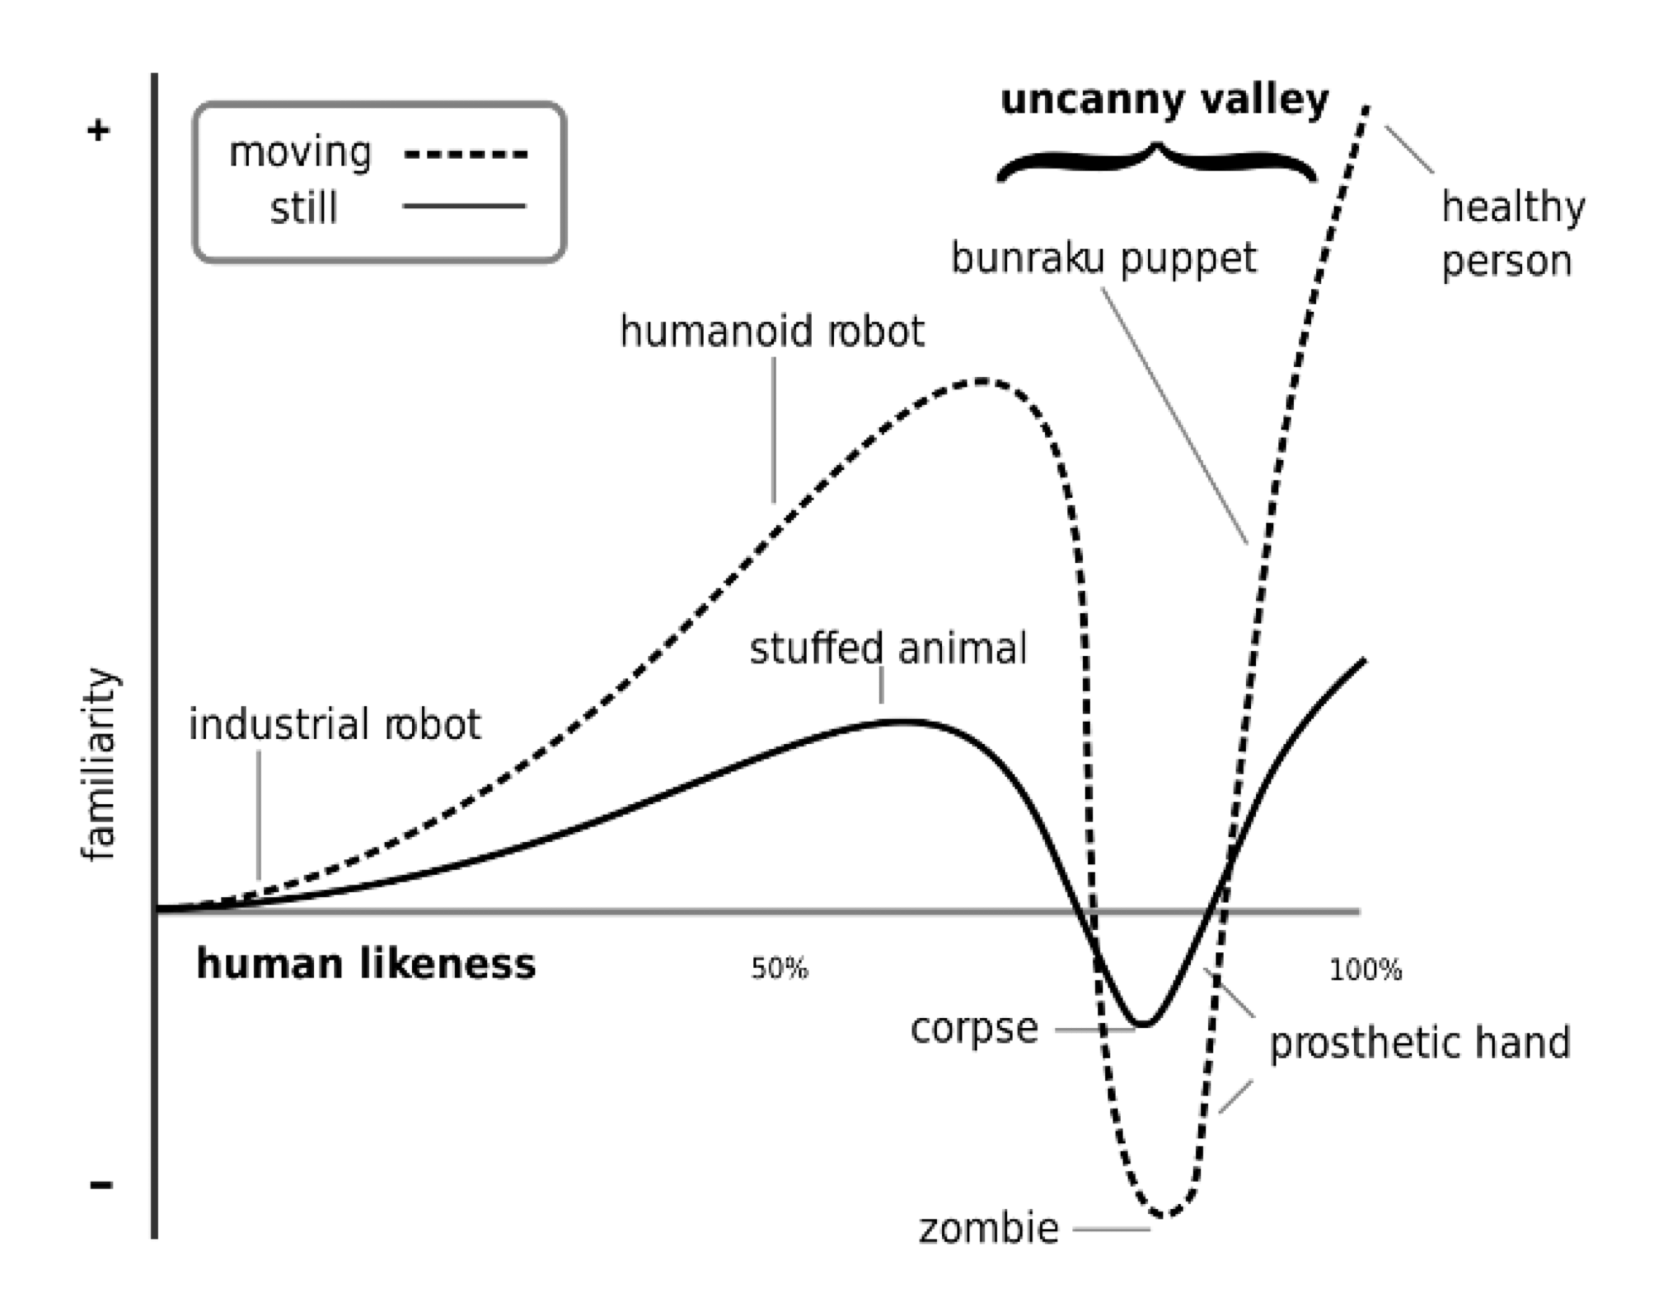
\includegraphics[width=1\textwidth]{figures/c4_divergent/diagrams/uncanny-valley.png}}
  \hfill
  \subfloat[]{\label{subfig:reversed-fine-tune}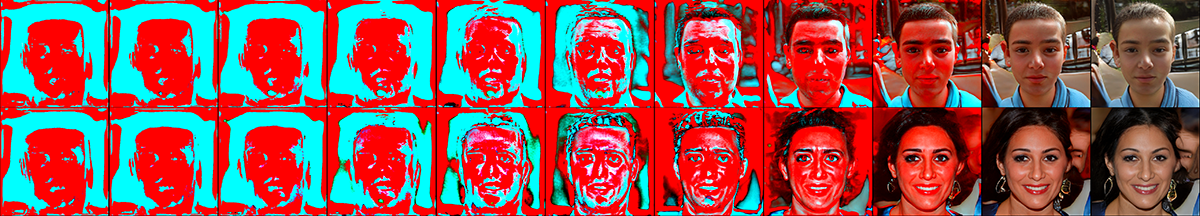
\includegraphics[width=1\textwidth]{figures/c4_divergent/diagrams/uncanny-valley-reverse-512-OG-B8.png}}
  \caption[Uncanny valley diagram juxtaposed with samples from fine-tuning process]{Uncanny valley diagram juxtaposed with fine-tuning samples in reverse order. (a) Diagram showing the uncanny valley \citep{mori1970uncanny}. (b) Samples from the fine-tuning procedure in Figure \ref{fig:c4:512-OG-samples} (512x512 finetuned with loss \ref{eq:inverted-adv-loss} with batch parameter 8) in reverse order. Diagram (a) reproduced under a CC BY-SA 3.0 licence. }
  \label{fig:c4:uncanny-valley-comparison}
\end{figure}

\section{Conclusion}

In this chapter, I have demonstrated an approach to fine-tuning pre-trained generative neural networks in a data-divergent fashion.
This approach was the first peer-reviewed and published method for divergent finetuning (to the best of my knowledge).
A complete account of other known methods for divergent finetuning to date is given in \S \ref{survey:divergent}.

While this work is novel, the results from all of the training runs described here are very idiosyncratic. 
The results are contingent on the unique state that the auxiliary models are in when their parameters are saved into checkpoints during training. 
In the case of the discriminator, this is completely unpredictable and not repeatable. 
While this can make for surprising outcomes, it also means that the experiments described would be impossible to reproduce without the exact model checkpoints (and sequence of latent that are sampled in fine-tuning).

How would it be possible then to manipulate a generative network in a way that was more controllable and repeatable?
This became a question that was playing on my mind after doing these experiments. 
The techniques described here use gradient descent to manipulate the weights of the model to produce novel outcomes. 
The process of gradient descent, however, is not something that we as humans can clearly understand, or easily control.
I became preoccupied with finding a way of manipulating generative models, without relying on gradient descent. 
The next chapter is the third and final chapter that details a novel technical contribution of in this thesis, one that centres humans in the creative process and allows them to manipulate generative neural networks without training of fine-tuning whatsoever.


\chapter{Network Bending: Direct and Expressive Manipulation of Generative Nediscussedural Networks}
\label{ch:net_bend}

\section{Introduction}

This chapter details the development of the \textit{network bending} framework. 
Which is a way to directly manipulate the internal features of generative neural networks during inference (Fig. \ref{fig:c5:overview_diagram} gives an overview of this process). 
This work was first published online as a pre-print on arxiv \citep{broad2020network} along with the source code on github\footnote{The source for the original StyleGAN2 network bending experiments is available at this URL: \url{https://github.com/terrybroad/network-bending}} then later a revised manuscript was accepted as a conference paper at EvoMUSART \citep{broad2021network}, and then as an extended journal paper in Entropy \citep{broad2022network}.
The experiments in the original paper were applied to the task of image generation with StyleGAN2 on models that were pre-trained on the Flickr-Faces High-Quality (FFHQ) \citep{karras2019analyzing} and  Large-scale Scene UNderstanding (LSUN) churches dataset \citep{yu2015lsun}. 
A follow-up study applying the same techniques to audio using a custom VAE trained on a dataset of varied musical genres (\S \ref{c5:sec:net-bend-audio}) was later completed for the extended Entropy paper. 
In this chapter, these experiments are documented chronologically.


\begin{figure}[!htb]
    \centering
    \includegraphics[width=1\textwidth]{figures/c5_netbend/misc/network-bending-diagram.png}
    \caption[Visual overview of the \textit{network bending} framework]{Visual overview of the \textit{network bending} framework, where deterministically controlled transformation layers can be inserted into a pre-trained network. As an example, a transformation layer that scales the activation maps by a factor of $k_x=k_y=0.6$ is applied (\S \ref{sec:affine}) to a set of features in layer 5 responsible for the generation of eyes, which has been discovered in an unsupervised fashion using the clustering algorithm to cluster features based on the spatial similarity of their activation maps (\S \ref{c5:sec:clustering}). Bottom left shows the sample generated by StyleGAN2 \citep{karras2019analyzing} trained on the FFHQ dataset without modification, while the image on the right shows the same sample generated with the scaling transform applied to the selected features. NB: the GAN network architecture diagram shown on the top row is for illustrative purposes only.}
    \label{fig:c5:overview_diagram}
\end{figure}

\section{Motivation}

Following the experiments detailed in Chapters \ref{ch:unstable_eq} \& \ref{ch:divergent}, I wanted to find an approach for actively diverging from data with generative neural networks, that was easier to control than methods that required the direct training or fine-tuning of the network itself.
In addition, whilst producing novel outputs, the previous approaches did not necessarily expand the possibility space of what could be generated in a way that was arguably superior to traditional generative modelling.
Both previous approaches focus on learning a set of weights that lead to reduced diversity in the generated outputs when compared with the successful training of a standard generative model such as a GAN or VAE.
The goal of the work described in this chapter was to find an approach that would expand the generative space, not shrink it. 


The inspiration for \textit{network bending} came from a conversation with my supervisor Mick Grierson.
After showing him the results detailed in the previous chapters, he said that though he liked the results, he was interested in methods that were more interactive and controllable, saying something along the lines of `I just want to stick my hand in the model and squeeze it, and see what pops out the other side' \citep{grierson2019personal}\footnote{According to Mick Grierson, the idea for network bending was also being discussed in MIMIC (Musically Intelligent Machines Interacting Creatively) research team meetings around the same time. I was not in those meetings so I cannot give an exactly chronology. However, many people clearly had similar ideas around this time as the idea of applying transformations to the activation maps of GANs was developed independently and concurrently developed by two others \citep{pinkney2020matlab,pouliot2020gan}.}. 
This statement stuck with me and eventually led to the development of the framework described here.

In some of the early experiments that led to this work, I hard-coded simple transformations into StyleGAN1 \citep{karras2019style} models during inference.
These early experiments (which later went on to become the series of artworks \textit{Teratome} \S \ref{c7:subsubsec:teratome}) sparked the intuition that eventually led to the implementation of many kinds of transformation layers (\S \ref{c5:sec:transforms}) and the clustering approach for grouping features together (\S \ref{c5:sec:clustering}).
The motivation for developing the clustering algorithm was the observation that when transformations were applied to random subsets of convolutional filters in a layer, then in some instances, manipulation of groups of filters had apparently powerful semantic effects, that could not be captured by only manipulating individual filters, as was done in the approach presented by \citep{bau2019semantic}.

In creating this framework, I wanted to give as much control and agency to people to manipulate generative neural networks as possible. 
The flexibility of this framework was key in order to achieve this, allowing for the expansion of the generative space of generative neural networks in a data-divergent fashion.

\section{Transformation Layers}

\label{c5:sec:transforms}

A key goal in this framework was to give as much direct control and agency to artists and creative practitioners as possible.
To maximise the amount of control people could have, I implemented a broad variety of deterministically controlled transformation layers that can be dynamically inserted into the computational graph of the generative model. 
The transformation layers are implemented natively in PyTorch \citep{paszke2019pytorch} for speed and efficiency. I
 treated the activation maps of each feature of the generative model as 1-channel images in the range -1 to 1. 
 Each transformation is applied to the activation maps individually before they are passed to the next layer of the network. 

 The transformation layers can be applied to all the features in a layer, or a random selection, or by using pre-defined groups automatically determined based on spatial similarity of the activation maps (\S \ref{c5:sec:clustering}). 
 Figure \ref{fig:c5:layerwide_comparison} shows a comparison of a selection of these transformations applied to all the features layer-wide in various layers of StyleGAN2.

\begin{figure}[htbp]
    \centering
    \includegraphics[width=1\textwidth]{figures/c5_netbend/misc/transform-comparison.png}
    \caption[Comparsion of various transformation layers applied in different layers of StyleGAN2]{A comparison of various transformation layers inserted and applied to all of the features in different layers in the StyleGAN2 network trained on the FFHQ dataset, showing how applying the same filters in different layers can make wide-ranging changes the generated output. The rotation transformation is applied by an angle $\theta=45$. The scale transformation is applied by a factor of $k_{x}=k_{y}=0.6$. The binary threshold transformation is applied with a threshold of $t=0.5$. The dilation transformation is applied with a structuring element with radius $r=2$ pixels.}
    \label{fig:c5:layerwide_comparison}
\end{figure}


\subsection{Pointwise Transformations}

I began with simple pointwise numerical transformations $f(x)$ that are applied to individual activation units $x$. 
I implemented four distinct numerical transformations: the first is \emph{ablation}, which can be interpreted as $f(x) = x \cdot 0$. 
The second is \emph{inversion}, which is implemented as $f(x) = 1 - x$. 
The third is \emph{multiplication by a scalar} $p$ implemented as $f(x) = x \cdot p$. 
The final transformation is \emph{binary thresholding} (often referred to  as posterisation) with threshold $t$, such that:
\begin{equation}
f(x) = \begin{cases}
    1,& \text{if  } x\geq t\\
    0,              & \text{otherwise}
\end{cases}
\end{equation}

\subsection{Affine Transformations}
\label{sec:affine}
For this set of transformations, each activation map $X$ for feature $f$ is treated as an individual matrix that simple affine transformations can be applied to. 
The first two are horizontal and vertical \emph{reflections} that are defined as:
\begin{equation}
X \begin{bmatrix}
-1 & 0 & 0\\
\ 0 & 1 & 0\\
\ 0 & 0 & 1
\end{bmatrix}\quad , \quad X \begin{bmatrix}
1 & \ 0 & 0\\
0 & -1 & 0\\
0 & \ 0 & 1
\end{bmatrix}
\end{equation}

\noindent The second is \emph{translations} by parameters $p_x$ and $p_y$ such that:
\begin{equation}
X \begin{bmatrix}
1 & 0 & p_x\\
0 & 1 & p_y\\
0 & 0 & 1
\end{bmatrix}
\end{equation}

\noindent The third is \emph{scaling} by parameters $k_x$ and $k_y$ such that:
\begin{equation}
X \begin{bmatrix}
k_x & 0 & 0\\
0 & k_y & 0\\
0 & 0 & 1
\end{bmatrix}
\end{equation}
Note that in this chapter, I only report on using uniform scalings, such that $k_x = k_y$. Finally, fourth is \emph{rotation} by an angle $\theta$ such that:
\begin{equation}
X \begin{bmatrix}
cos(\theta) & -sin(\theta) & 0\\
sin(\theta) & cos(\theta) & 0\\
0 & 0 & 1
\end{bmatrix}
\end{equation}

\subsection{Morphological Transformations}

I implemented two of the possible basic mathematical morphological transformation layers, performing \emph{erosion} and \emph{dilation} \citep{soille1999erosion} when applied to the activation maps, which can be interpreted as 1-channel images  (Fig. \ref{fig:c5:morphological transforms}). 
These can be configured with the parameter $r$ which is the radius for a circular kernel (aka structural element) used in the morphological transformations.

\begin{figure}[!htb]
    \centering
    \subfloat[]{\label{subfig:morph-a}\includegraphics[width=.32\textwidth]{figures/c5_netbend/morphology_activations/original_007.png}}
    \hfill
    \subfloat[]{\label{subfig:morph-a-erode}\includegraphics[width=.32\textwidth]{figures/c5_netbend/morphology_activations/erode_007.png}}
    \hfill
    \subfloat[]{\label{subfig:morph-a-dilate}\includegraphics[width=.32\textwidth]{figures/c5_netbend/morphology_activations/dilate_007.png}}
    \caption[Examples of morphological transformations being applied to an individual activation map in Layer 10 of StyleGAN2]{Examples of morphological transformations being applied to an individual activation map in Layer 10 of StyleGAN2. (a) Unmodified activation maps. (b) Activation map after erosion was applied ($r=2$ pixels). (c) Activation maps after dilation were applied ($r=2$ pixels).}
    \label{fig:c5:morphological transforms}
 \end{figure}

\section{Clustering Features}
\label{c5:section:clustering}

As most of the layers in the current state-of-the-art generative models, such as StyleGAN2, have very large numbers of convolutional features, controlling each one individually would be far too complicated to build a user interface around and control these in a meaningful way. 
In addition, because of the redundancy existing in these models, manipulating individual features does not normally produce any kind of meaningful outcome.\footnote{I discovered this through my early hard-coded experiments with network bending that are discussed in Section \ref{c7:subsubsec:teratome}.} 
Therefore, it is necessary to find some way of grouping them into more manageable ensembles of sets of features. 
Ideally, such sets of features would correspond to the generation of distinct, semantically meaningful aspects of the image, and manipulating each set would correspond to the manipulation of specific semantic properties in the resulting generated sample. 
To achieve this, I developed a novel approach that combines metric learning and a clustering algorithm to group sets of features in each layer based on the spatial similarity of their activation maps. 
I trained a separate convolutional neural network (CNN) for each layer of StyleGAN2 to analyse the appearance of the activation maps. 
The CNN has a bottleneck architecture (first introduced by Gr{\'e}zl et al.~\citep{grezl2007probabilistic}) to learn a highly compressed feature representation; the latter is then used in a metric learning approach in combination with the $k$-means clustering algorithm \citep{lloyd1982least, celebi2013comparative} to group sets of features in an unsupervised fashion. 

\subsection{Architecture}

For each layer of StyleGAN2, I trained a separate CNN on the activation maps of all the convolutional features. 
The resolution of the activation maps and the number of convolutional features varies for the different layers of the model (a breakdown of which can be seen in Table \ref{tab:classifier-table}).
I employed an architecture that can dynamically be changed, by increasing the number of convolutional blocks, depending on what depth is required. 

\begin{table}[]
\centering
\begin{tabular}{|c|c|c|c|c|c|}%{llllll}
\hline
Layer & Resolution & \#features &  CNN depth & \#clusters & Batch size\\
\hline
1     & 8x8        & 512          & 1                & 5                & 500        \\
2     & 8x8        & 512          & 1                & 5                & 500        \\
3     & 16x16      & 512          & 2                & 5                & 500        \\
4     & 16x16      & 512          & 2                & 5                & 500        \\
5     & 32x32      & 512          & 3                & 5                & 500        \\
6     & 32x32      & 512          & 3                & 5                & 500        \\
7     & 64x64      & 512          & 4                & 5                & 200        \\
8     & 64x64      & 512          & 4                & 5                & 200         \\
9     & 128x128    & 256          & 5                & 4                & 80         \\
10    & 128x128    & 256          & 5                & 4                & 80         \\
11    & 256x256    & 128          & 6                & 4                & 50         \\
12    & 256x256    & 128          & 6                & 4                & 50         \\
13    & 512x512    & 64           & 7                & 3                & 20         \\
14    & 512x512    & 64           & 7                & 3                & 20         \\
15    & 1024x1024  & 32           & 8                & 3                & 10         \\
16    & 1024x1024  & 32           & 8                & 3                & 10       \\
\hline
\end{tabular}
\medskip
\caption[Table detailing model architecture for the ShuffleNet models used for clustering in StyleGAN2.]{
    \label{tab:classifier-table}Table showing resolution, number of features of each layer, the number of ShuffleNet \citep{zhang2018shufflenet} convolutional blocks for each CNN model used for metric learning, the number of clusters calculated for each layer using $k$-means and the batch size used for training the CNN classifiers for the StyleGAN2 models. Note: LSUN church and cat models have only 12 layers.
%\citep{lloyd1982least, celebi2013comparative}.
}
\end{table}

I employed the ShuffleNet architecture \citep{zhang2018shufflenet} for the convolutional blocks in the network. 
For each convolutional block, I utilised a feature depth of 50 and had one residual block per layer. 
The motivating factor in many of the decisions made for the architecture design was not focused on achieving the best accuracy per se. 
Instead, I wanted a network that could learn a sufficiently good metric while also being reasonably quick to train (with 12-16 separate classifiers required to be trained per the StyleGAN2 model). 
I also wanted a lightweight enough network, such that it could be used in a real-time setting where clusters can quickly be calculated for an individual latent encoding, or when processing large batches of samples.

After the convolutional blocks, I flattened the final layer and used this to learn a mapping into a narrow bottleneck $\vec{v} \in \mathbb{R}^{10}$, before re-expanding the dimensionality of the final layer to the number of convolutional features present in the layer of the respective generative model. 
The goal of this bottleneck is to force the network to learn a highly compressed representation of the different convolutional features in the generative model. 
While this invariably loses some information, most likely negatively affecting classification performance during training, this is in fact the desired result. 
I wanted to force the CNN to combine features of the activation maps with similar spatial characteristics so that they can easily be grouped by the clustering algorithm. 
Another motivating factor is that the chosen clustering algorithm ($k$-means) does not scale well for feature spaces with high dimensionality.

\subsection{Training}

I generated a training set of the activations of every feature for every layer of 1000 randomly sampled images and a test set of 100 samples for the models trained on all of the datasets used in these experiments. 
I trained each CNN using the softmax feature learning approach \citep{dosovitskiy2014discriminative}, a reliable method for distance metric learning. This method employs the standard softmax training regime \citep{bridle1990probabilistic} for CNN classifiers. 
Each classifier has been initialised with random weights and then trained for 100 epochs using the Adam optimiser \citep{kingma2015adam} with a learning rate of 0.0001 and with $\beta_1 = 0.9$ and $\beta_2 = 0.999$. 
All experiments were carried out on a single NVIDIA GTX 1080ti. The batch size used for training the classifiers for the various layers of StyleGAN2 can be seen in Table \ref{tab:classifier-table}. 
% The classifiers for the VAE were all trained with a batch size of 100.

After training, the softmax layer is discarded and the embedding of the bottleneck layer is used as the discriminative feature vector where the distances between points in feature space permit gauging the degree of similarity of two samples. 
This approach differs from standard softmax feature learning as it uses the feature vector from the bottleneck, rather than the last layer prior to softmax classification, giving a more compressed feature representation than the standard softmax feature learning approach.

\subsection{Clustering Algorithm}

\label{c5:sec:clustering}

Once each of the CNNs for every layer has been trained, they can then be used to extract feature representations of the activation maps of the different convolutional features corresponding to each layer of the generative model.
The approach is to perform clustering based on an average of features' embeddings drawn from many random samples, which can be used to find a general-purpose set of clusters for a trained model.

The activation map $X_{df}$ for each layer $d$ and feature $f$ is fed into the CNN metric learning model for that layer $C_d$ to get the feature vector $\vec{v}_{df}$. 
This process is repeated N times (1000 in these experiments) to find the mean feature vector $\vec{\bar{v}}_{df}$ for each convolutional filter.
The mean feature vectors for each filter in each layer are then aggregated and fed to the $k$-means clustering algorithm --- using Lloyd's method \citep{lloyd1982least} with Forgy initialization \citep{forgy1965cluster, celebi2013comparative}. 

The predetermined number of clusters for each layer in StyleGAN2 can be seen in Table \ref{tab:classifier-table}. 
Examples from the clustering algorithm applied to the FFHQ StyleGAN2 model can be seen in Figure \ref{fig:c5:cluster_layer_comp_image}.

\begin{figure}[!htbp]
    \centering
        \subfloat[]{\includegraphics[width=.24\textwidth]{figures/c5_netbend/cluster_comparison/not_manipulated.png}}
        \hfill
        \subfloat[]{\includegraphics[width=.24\textwidth]{figures/c5_netbend/cluster_comparison/layer_1_cluster0_mult-1.png}}
        \hfill
        \subfloat[]{\includegraphics[width=.24\textwidth]{figures/c5_netbend/cluster_comparison/layer_3_cluster2_mult5.png}}
        \hfill
        \subfloat[]{\includegraphics[width=.24\textwidth]{figures/c5_netbend/cluster_comparison/layer_5_cluster2_ablate.png}}
        \hfill
        \subfloat[]{ \includegraphics[width=.24\textwidth]{figures/c5_netbend/cluster_comparison/layer_6_cluster4_dilate.png}}
        \hfill
        \subfloat[]{ \includegraphics[width=.24\textwidth]{figures/c5_netbend/cluster_comparison/layer_9_cluster3_mult5.png}}
        \hfill
        \subfloat[]{\includegraphics[width=.24\textwidth]{figures/c5_netbend/cluster_comparison/layer_10_cluster0_mult-1.png}}
        \hfill
        \subfloat[]{\includegraphics[width=.24\textwidth]{figures/c5_netbend/cluster_comparison/layer_15_cluster0_mult0.1.png}}
       \caption[A comparison of different transforms being applied to different clusters in various layers of StyleGAN2]{Examples from the clustering algorithm in the image domain. Clusters of features in different layers of the model are responsible for the formation of different image attributes. (a) The unmanipulated result. (b) A cluster in layer 1 has been multiplied by a factor of -1 to completely remove the facial features. (c) A cluster in layer 3 has been multiplied by a factor of 5 to deform the spatial formation of the face. (d) A cluster in layer 6 has been ablated to remove the eyes. (e) A cluster in layer 6 has been dilated with a structuring element with radius $r=2$ pixels to enlarge the nose. (f) A cluster in layer 9 has been multiplied by a factor of 5 to distort the formation of textures and edges. (g) A cluster of features in layer 10 has been multiplied by a factor of -1 to invert the highlights on facial regions. (h) A cluster of features in layer 15 has been multiplied by a factor of 0.1 to desaturate the image. All transformations have been applied to sets of features discovered using the feature clustering algorithm (\S \ref{c5:section:clustering}) in the StyleGAN2 model trained on the FFHQ dataset.}
       \label{fig:c5:cluster_layer_comp_image}
    \end{figure}

The main motivation of the clustering algorithm presented in this paper was to simplify the parameter space in a way that allows for more meaningful and controllable manipulations whilst also enhancing the expressive possibilities afforded by interacting with the system. 
These results show that the clustering algorithm is capable of discovering groups of features that correspond to the generation of different semantic aspects of the results, which can then be manipulated in tandem. 
These semantic properties are discovered in an unsupervised fashion and across the entire hierarchy of features present in the generative model.
Figure \ref{fig:c5:cluster_layer_comp_image} shows the manipulation of groups of features across a broad range of layers that control the generation of the entire face, the spatial formation of facial features, the eyes, the nose, textures, facial highlights and overall image contrast.

\section{Manipulation Pipeline}

Transforms are specified in YAML (YAML Ain't Markup Language) configuration files \citep{ben2009yaml} (Fig. \ref{fig:c5:yaml-transform-config} for an example of one of these configs), such that each transform is specified with 5 items: (i) the layer, (ii) the transform itself, (iii) the transform parameters, (iv) the layer type (i.e. how the features are selected in the layer: across all features in a layer, to pre-defined clusters, or to a random selection of features), and (v) the parameter associated with the layer type (either the cluster index, or the percentage of features the filter will randomly be applied to). 
Visual examples of how different layer types can be seen in Figure \ref{fig:c5:layer-transform-types}.
There can be any number of transforms defined in such a configuration file and transforms can be chained together to produce more complex filtering effects in the generated output  (Fig. \ref{subfig:chaining-transformations}).

After loading the configuration, the software either looks up which features are in the cluster index or randomly applies indices based on the random threshold parameter. 
Then the latent is loaded, which can either be randomly generated, or be predefined in latent space $z$, or be calculated using a projection in latent space $w$ \citep{abdal2019image2stylegan,karras2019analyzing} (in the case of StyleGAN2). The latent code is provided to the generator network and inference is performed. 
As this implementation uses PyTorch \citep{paszke2019pytorch}, a dynamic neural network library, these transformation layers can therefore be inserted dynamically during inference as and when they are required and applied only to the specified features as defined by the configuration. 
Once inference is unrolled, the generated output is returned. Figure \ref{fig:c5:overview_diagram} provides a visual overview of the pipeline, as well as a comparison between a modified and unmodified generated sample.

\begin{figure}[!htb]
    \centering
    \subfloat[]{\label{subfig:layer-wide}\includegraphics[width=.24\textwidth]{figures/c5_netbend/layer-transform-types/layer-wide.png}}
    \hfill
    \subfloat[]{\label{subfig:random-layer}\includegraphics[width=.24\textwidth]{figures/c5_netbend/layer-transform-types/stochastic.png}}
    \hfill
    \subfloat[]{\label{subfig:cluster-layer}\includegraphics[width=.24\textwidth]{figures/c5_netbend/layer-transform-types/cluster.png}}
    \hfill
    \subfloat[]{\label{subfig:chaining-transformations}\includegraphics[width=.24\textwidth]{figures/c5_netbend/layer-transform-types/chaining-transforms.png}}
    \caption[Examples of transformation layers being applied to different configurations of features]{Examples of transformation layers being applied to different configurations of features in StyleGAN2. (a) Transformation applied layer-wide. (b) Transformation is applied to a random selection of filters in one layer. (c) Transformation applied to a cluster in layer 2. (d) A combination of transformation layers applied across a network, the configuration of transformations used to generate this image can be seen in Figure \ref{fig:c5:yaml-transform-config}.}
    \label{fig:c5:layer-transform-types}
 \end{figure}

 \begin{figure}[!htb]
 \begin{lstlisting}[language=yaml]
    ---
    transforms:
    - layer: 2
      transform: "invert"
      params: []
      features: "all"
      feature-param: 
    - layer: 6
      transform: "binary-thresh"
      params: [0.5]
      features: "random"
      feature-param: 0.5
    - layer: 6
      transform: "scalar-multiply"
      params: [5]
      features: "cluster"
      feature-param: 2
    ---
    \end{lstlisting}
    \caption[Example YAML transformation config]{Example of a YAML transformation config that is used in the network bending framework. This config combines randomly applied layers and layer-wide transformations. This config was used to generate the image Figure \ref{subfig:chaining-transformations}.}
    \label{fig:c5:yaml-transform-config}
 \end{figure}

\section{Network Bending in the Audio Domain}
\label{c5:sec:net-bend-audio}

As a follow-up study to the original network bending approach on images, I applied the same approach to the audio domain as an extension to the work for the journal paper in Entropy \citep{broad2022network}. 
The motivation for this was to demonstrate that network bending was applicable to different types of media and to demonstrate the general-purpose nature of this framework. 

For this study, I trained a custom VAE model on spectrograms of music and applied the exact same algorithm for clustering and applying the same transformation layers as was applied in network bending for image generation. 
Network bending has also been applied to audio by other researchers and practitioners, this efforts are detailed in Sections \ref{c7:subsubsec:naotokui} \& \ref{c7:subsubsec:ddsp}.

\subsection{Custom Audio Model}

For this experiment, I trained a variational autoencoder (VAE) \citep{kingma2013auto,rezende2014stochastic} on spectrograms extracted from a custom dataset of varied musical genres, totalling 3461 audio tracks. This approach is based on previous methods for learning generative models of spectrograms \citep{akten2018granma} and Mel spectrograms \citep{valenzuela2021melspecvae} with VAEs. The tracks are randomly split up into short sequences and the Fourier transform is performed with a hop size of 256 and a window size of 1024 to produce spectrograms that have a bin size of 513. The spectrograms are then cut into shorter sequences of a window length of 128. These shortened spectrograms are then converted to decibels and then normalised for training with the VAE.  

The VAE was built using a convolutional architecture with a latent vector with dimension $\vec{v} \in \mathbb{R}^{512}$. The encoder has 5 layers that use standard convolutions with a kernel size of 5x5, a stride of 2x2 and no padding for all of the layers. The decoder uses transposed convolutions, and Table \ref{tab:c5:decoder-architecture} lists the output resolution, kernel size, stride, and padding parameters for each of the 5 convolutional layers. A fully connected layer is used in both the encoder and decoder to interface between the convolutional layers and the latent vector. The model was trained for 50 epochs on the dataset with batch normalisation using a batch size of 64. The model was trained using the Adam optimiser \citep{kingma2014adam} with a learning rate of 0.0003 and with $\beta_1 = 0$ and $\beta_2 = 0.99$.

After training it is possible to sample randomly in the latent space and then sample directly from the decoder. It is also possible to input audio sequences, both from the training set and outside of it, and produce reconstructions of the audio track mediated through the VAE model, in a method that I have previously referred to as \textit{autoencoding} \citep{broad2017autoencoding}. Performing this autoencoding procedure in combination with network bending, provides a new way of transforming and filtering audio.

\begin{table*}[]
    \centering
    \begin{tabular}{|c|c|c|c|c|c|c|c|}
    \hline
    Layer & Resolution & \#features & kernel size & stride & padding \\
    \hline
    1     & 8x33       & 512        & 5x5         & 1x2     & 0x2  \\
    2     & 17x65      & 256        & 3x5         & 2x2     & 2x2 \\
    3     & 32x129     & 128        & 4x5         & 2x2     & 2x2 \\
    4     & 64x257     & 64         & 4x5         & 2x2     & 2x2  \\
    5     & 128x513    & 1          & 4x5         & 2x2     & 2x2  \\
    \hline
    \end{tabular}
    \medskip
    \caption{\label{tab:c5:decoder-architecture}Table showing resolution, number of features of each layer, convolutional kernel size, strides, and padding parameters for the decoder network in the spectrogram VAE.}
    
    \end{table*}

\subsection{Clustering}

the approach to clustering for this audio model was identical to what was demonstrated in Section \ref{c5:section:clustering}.
As the VAE model did not have as many layers as StyleGAN2, clusters were only calculated for four layers, the details of which can be seen in Table \ref{tab:c5:audio-clustering}.

\begin{table*}[]
    \centering
    \begin{tabular}{|c|c|c|c|c|c|c|c|}
    \hline
    Layer & CNN Depth & \#clusters \\
    \hline
    1     & 1 &   5 \\
    2     & 2 &   5 \\
    3     & 3 &   4 \\
    4     & 4 &  4 \\
    \hline
    \end{tabular}
    \medskip
    \caption{\label{tab:c5:audio-clustering}Table showing the number of ShuffleNet \citep{zhang2018shufflenet} convolutional blocks for each CNN model used for metric learning and the number of clusters calculated for each layer using $k$-means.}
    
    \end{table*}

\subsection{Results}

The clustering approach applied to the audio model appears to work well when visualising the spectrograms, and it is clear that this approach can capture and manipulate some semantically meaningful components in the audio signal\footnote{Unfortunately there was a bug in the decoding of the spectrograms back into audio which meant that the audio quality in the generated samples was very noisy -- something that I have not been able to fix.}  (Fig. \ref{fig:c5:cluster_audio_comp}). 
Not all of the transformations that can be applied to images work as well in audio, such as scaling and rotation.
This is not a surprise given that the location of each pixel is essential information used to represent frequency and time information in the audio signal, and can completely transform the information represented when manipulated.
However, the morphological transformations do at least preserve locality in the signal, and using these filters in generative models of spectrograms offers a completely new way to transform audio signals.

\begin{figure}[tp!]
\vspace{-80pt}
\centering
    \subfloat[]{\includegraphics[width=.4\textwidth]{figures/c5_netbend/audio_clusters/soul_short_original.png}}
    \hfill
    \subfloat[]{\includegraphics[width=.4\textwidth]{figures/c5_netbend/audio_clusters/soul_short_reconstruction.png}}
   \hfill
    \subfloat[]{\includegraphics[width=.4\textwidth]{figures/c5_netbend/audio_clusters/layer_1_cluster3_ablate.png}}
    \hfill
    \subfloat[]{\includegraphics[width=.4\textwidth]{figures/c5_netbend/audio_clusters/layer_1_cluster3_mult_2.png}}
   \hfill
    \subfloat[]{\includegraphics[width=.4\textwidth]{figures/c5_netbend/audio_clusters/layer_3_cluster2_erode.png}}
    \hfill
    \subfloat[]{\includegraphics[width=.4\textwidth]{figures/c5_netbend/audio_clusters/layer_3_cluster2_dilate.png}}
   \caption[A comparison of different transforms being applied to different clusters in various layers of the SpectrogramVAE]{Examples from the clustering approach in the audio domain. (a) Spectrogram of an original source track not in the training set. (b) Reconstruction of source track using VAE without manipulation. (c) Reconstruction of the same signal where a cluster in layer 1 responsible for the generation of the transients of the signal has been ablated. (d) Reconstruction of the same signal where the same cluster in layer 1 responsible for the transients has been multiplied by a factor of 2, increasing the intensity of the transients in the resulting signal. (e) Reconstruction of the signal where a cluster in layer 3 responsible for the low and mid-range frequencies has been eroded with a structuring element with radius $r=2$ pixels, diminishing the intensity of these frequency components. (f) Reconstruction of the signal where the same cluster in layer 3 responsible for the low and mid-range frequencies has been dilated with a structuring element with radius $r=2$ pixels, increasing the intensity of these frequency components. The audio sample used is a clip from \textit{Saulsalita Soul} by Mr.RuiZ, reproduced and transformed with permission granted under the CC BY-NC 4.0 licence.}
   \label{fig:c5:cluster_audio_comp}
\end{figure}

\section{Discussion}

In this section, I discuss several different perspectives on the outcomes presented here: expressive manipulation, active divergence, comparisons of the results between the image and audio domains, and comparisons with other methods.

\subsection{Expressive Manipulation}

The main motivation of the clustering algorithm presented in this chapter was to simplify the parameter space in a way that allows for more meaningful and controllable manipulations whilst also enhancing the expressive possibilities afforded by interacting with the system. 
These results show that the clustering algorithm is capable of discovering groups of features that correspond to the generation of different semantic aspects of the results, which can then be manipulated in tandem. 
These semantic properties are discovered in an unsupervised fashion and across the entire hierarchy of features present in the generative model.
For example, Figure \ref{fig:c5:cluster_layer_comp_image} shows the manipulation of groups of features across a broad range of layers that control the generation of the entire face, the spatial formation of facial features, the eyes, the nose, textures, facial highlights and overall image contrast. Figure \ref{fig:c5:cluster_audio_comp} shows the clustering algorithm performed in the audio domain, to demonstrate how aspects of the audio signal such as the transients and frequency components can be manipulated with various kinds of transformations.

Grouping and manipulating features in a semantically meaningful fashion is an important component of allowing expressive manipulation. 
However, artists are often also ready to consider surprising, unexpected results, to allow for the creation of new aesthetic styles, which can become uniquely associated with an individual or group of creators. 
Therefore the tool needs to allow for unpredictable as well as predictable possibilities, which can be used in an exploratory fashion and can be mastered through dedicated and prolonged use \citep{dobrian2006nime}. 
There is usually a balance between the utility and expressiveness of a system \citep{jacobs2017supporting}. 

Section \ref{c7:sec:net-bend-artworks} shows the various different ways this framework has been used to make artworks.
Whilst I did not make a user interface for network bending myself, many other researchers have gone on to do so.
Their efforts are detailed in Section \ref{c7:subsec:net-bend-interfaces}.

\subsection{Comparison Between Audio and Image Domains}

In this chapter, I have described the network bending framework in both the image and audio domains. 
For the image domain, I have used StyleGAN2 \citep{karras2019analyzing}, the state of the art generative model for unconditional image generation. In the audio domain, I have built a custom generative model to demonstrate how the same principles of clustering features and applying transformations to clustered features can be applied indirectly to another domain. 
The generative model for audio I have presented is building on a much smaller body of research and has more room for improvement in terms of the fidelity of the generated outputs, however, it is still adequate and demonstrates that the clustering algorithm is capable of discovering semantically meaningful components of the signal  (Fig. \ref{fig:c5:cluster_audio_comp}). 
Some of the transformation layers that were designed for image-based models such as rotation and scaling do not transfer meaningfully into the audio domain. 
However, numerical and morphological transformations do work effectively in the audio domain, representing a completely new approach for manipulating audio signals. 
In addition to my efforts, other researchers have also gone on to successfully implement network bending in audio models (\S \ref{c7:subsubsec:naotokui} \& \S \ref{c7:subsubsec:ddsp}).

\subsection{Comparison with Other Methods}

With respect to the semantic analysis and manipulation of a generative model, this approach of clustering features and using a broad array of transformation layers is a significant advance over previous works \citep{Bau2017-vg,Bau2018-td,bau2019semantic, Brink2019-gc}. 
This recent thread of techniques only interrogates the function of individual features, and as such is unlikely to be capable of capturing a full account of how a deep network generates results since such networks tend to be robust to the transformation of individual features. 

The results in this chapter show that sets of features, which may not be particularly responsive to certain transformations, are very responsive to others. 
Figure \ref{fig:c5:ablation_comp} shows that in the model trained on the LSUN church dataset, a cluster of features, when ablated, have little noticeable effect on the result.
However, significant changes are visible when using the pointwise scalar multiplication transformation on the same cluster, here removing the trees and revealing the church building that was obscured by the foliage in the original result. 
The clustering approach described in this paper suggests that the functionality of features, or sets of features, cannot be understood only through ablation, because of the high levels of redundancy present in the learned network parameters. 
In addition, the research here shows that their functionality can be better understood by applying a wide range of deterministic transformations, of which different transformations, some of which are better suited to revealing the utility of different sets of features (Figs. \ref{fig:c5:cluster_layer_comp_image} \& \ref{fig:c5:ablation_comp}). 
An approach that has since been developed further by \cite{oldfield2022panda,oldfield2024bilinear}.

\begin{figure}[!htbp]
   \centering
   \subfloat[]{\includegraphics[width=.32\textwidth]{figures/c5_netbend/church_ablation_comparison/not_manipulated.png}}
   \hfill
   \subfloat[]{\includegraphics[width=.32\textwidth]{figures/c5_netbend/church_ablation_comparison/layer_3_cluster1_ablate.png}}
   \hfill
   \subfloat[]{\includegraphics[width=.32\textwidth]{figures/c5_netbend/church_ablation_comparison/layer_3_cluster1_mult5.png}}
   \caption[A comparison of one cluster in StyleGAN2 having two different transforms applied to it]{Groups of features that are not particularly sensitive to ablation may be more sensitive to other kinds of transformation. (a) Original unmodified input. (b) A cluster of features in layer 3 that has been ablated. (c) The same cluster of features that has been multiplied by a scalar of 5. As can be seen, ablation had a negligible effect, only removing a small roof structure that was behind the foliage. On the other hand, multiplying by a factor of 5 removes the trees whilst altering the building structure to have gable roof sections on both the left and right sides of the church - which are now more prominent and take precedence in the generative process. Samples are taken from the StyleGAN2 model trained on the LSUN church dataset.}
   \label{fig:c5:ablation_comp}
\end{figure}

This method of analysis is completely \emph{unsupervised} and does not rely on auxiliary models trained on large labelled datasets (such as in \citep{Bau2018-td, isola2017image, park2019semantic}) or other kinds of domain-specific knowledge. 
This approach therefore can be applied to any CNN-based generative model architecture which has been trained on any dataset, as I have demonstrated by using the exact same clustering method for both image and audio domains. 
This is of particular relevance to artists who create their own datasets and would want to apply these techniques to models they have trained on their own data. 
Labelled datasets are prohibitively time-consuming (and expensive) to produce for all but a few individuals or organisations. 
Having a method of analysis that is completely unsupervised and can be applied to unconditional generative models is important in opening up the possibility for such techniques to become adopted more broadly.
Section \ref{c7:sec:net-bend-artworks} details a number of artworks made by myself and others, applied to a range of datasets, both preexisting and custom.
The limitation of this approach is the time and computational resources needed to train a separate model for each layer of the network.
This limitation is discussed further in Section \ref{c9:sec:limitations}, and ways to improve upon this are further presented in Section \ref{c9:sec:future}.


\section{Conclusion}

In this chapter, I have introduced a novel approach for the interaction with and manipulation of generative neural networks, which has been demonstrated in both the image and audio domains. 
By inserting deterministic filters inside pre-trained neural networks, this framework allows for manipulation to be performed inside the networks' `black-box', generating samples that have no resemblance to the training data, or anything that could be created easily using conventional media editing software. 
This chapter also presents a novel clustering algorithm that can group sets of features in an unsupervised fashion, based on the spatial similarity of their activation maps. 
I have demonstrated that this method is capable of finding sets of features that correspond to the generation of a broad array of semantically significant aspects of the generated results in both image and audio domains. 

The goal of the work in this thesis was to find a way to expand the possibility space of what can be generated with neural networks.
\textit{Network bending} is an approach that expands the generative space of existing pre-trained models in a way that gives direct control and agency to artists and creative practitioners, and in a way that \textit{actively diverges} from data.
This now concludes the documentation of new algorithms and approaches to \textit{active divergence} presented in this thesis. 
The next chapter will a broader perspective, contextualising the work in this thesis with other related efforts that occurred during its development.
Chapter \ref{ch:active_div} gives a detailed survey and taxonomy of active divergence methods, placing the work presented in this thesis into a larger context and delineating and outlining the landscape of active divergence methods to date. 


\chapter*{Interlude}
\addcontentsline{toc}{chapter}{Interlude}
\label{ch:interlude}



\chapter{Surveying The Active Divergence Landscape}
\label{ch:active_div}

\section{Introduction}

\section{Generative Models: A Statisical View}

While not all generative models rely on generative deep learning, we refer here to those that build on artificial neural networks\footnote{
    For further reading, a comprehensive overview of generative models is given in \citet{harshvardhan2020comprehensive}.}. 
Given a data distribution $P$, a generative model will model an approximate distribution $P'$. 
The parameters for the approximate distribution can be learned by an artificial neural network. 
This learning task is tackled differently by different architectures and training schemes. 
E.g. autoencoders \citep{rumelhart1985learning} and variational autoencoders (VAE) \citep{kingma2013auto,rezende2014stochastic} learn to approximate the data through reconstruction via an encoding and a decoding network, while generative adversarial networks (GAN) \citep{goodfellow2014generative} consists of a generator that is guided by a discriminating network. 
In most cases, the network learns a mapping from a lower-dimensional latent distribution $X$ to the complex high-dimensional feature space of a domain. 
The model, thus, generates a sample $p'$ given an input vector $x$ which should resemble samples drawn from the target distribution $P$. 
In the simplest case of a one layer network the generated sample $p'$ is generated using the function: $p' = \sigma(Wx+b)$ where $x$ is the input vector from the latent distribution $x \in X$, $\sigma$ is a non-linear activation function, $W$ and $b$ are the learned association matrix and bias vector for generating samples in the approximate distribution $p' \in P'$. 
The model parameters $W$ and $b$, are typically learned through gradient-based optimisation process. 
In this process, a loss function will require the model to maximise the likelihood of the data either: (i) explicitly, as in the case of autoencoders, autoregressive \citep{frey1996does} and flow-based generative models \citep{dinh2014nice}; (ii) approximately, as is the case in VAEs; (iii) or implicitly, as in the case of GANs. Generative models can also be conditioned on labelled data. In the conditional case, the generative model takes two inputs $x$ and $y$, where $y$ represents the class label vector. 
Another form of conditional generative models are translation models, such as pix2pix \citep{isola2017image}, that takes a (high dimensional) data distribution as input $Q$ and learns a mapping to $P'$ which is an approximation of the true target function $f: Q \rightarrow P$.

\begin{figure}[!htbp]
    \centering
    \includegraphics[width=1\textwidth]{figures/c2_background/diagrams/training_gen_model_distro_view.png}
    \caption[Diagram illustrating the distribution view of training a generative model.]{Diagram illustrating the parameter view of training a generative model. \textbf{Left:} The true distribution \textcolor{blue}{$P$}. \textbf{Middle:} The approximate distribution \textcolor{green}{$P'$}. \textbf{Right:} The approximate distribution \textcolor{green}{$P'$} overlayed on the true distribution \textcolor{blue}{$P$}.}
  \label{fig:c6:gen-model-distribution-view}
  \end{figure}

\begin{figure}[!htbp]
    \centering
    \includegraphics[width=1\textwidth]{figures/c2_background/diagrams/training_generative_model_parameter_view.png}
    \caption[Diagram illustrating the parameter view of training a generative model.]{Diagram illustrating the parameter view of training a generative model. A network with randomly initialised parameters is trained to model the true distribution $P$ and produces the approximate distribution \textcolor{blue}{$P'$}}.
  \label{fig:c6:gen-model-parameter-view}
  \end{figure}

All deep generative models, and in particular ones that generate high dimensional data domains like images, audio and natural language, will have some level of divergence $D(P||P') \geq 0$ between the target distribution $P$ and the approximate distribution $P'$, because of the complexity and stochasticity inherent in high dimensional data. 
The goal of all generative models is to minimise that level of divergence, by maximising the likelihood of generating the given data domain. 
Active divergence methods however, intentionally seek to create a new distribution $U$ that does not directly approximate a given distribution $P$, or resemble any other known data distribution. 
This is either done by seeking to find model parameters $W^*$ and $b^*$ (in the single layer case) that generate novel samples $u = \sigma(W^*x+b^*)$, or by making other kinds of interventions to the chain of computations.

% \subsection{Survey of Active Divergence Methods}

% We present a comprehensive overview and taxonomy of the state of the art in methods for achieving active divergence. 
% In this survey, we will use the term divergence in the statistical sense, as being the distance (or difference) between two distributions. 
% There are other definitions of divergence relevant to research in creativity, such as Guildford's dimensions of divergent thought \citep{hocevar1980intelligence}. 
% While there are some parallels that can be drawn between some of the active divergence methods, and theories of divergent thinking; for the clarity of technical exposition, we will be sticking strictly to the statistical definition of divergence in this overview of active divergence methods. 

\section{Taxonomy of Active Divergence Methods}

This section presents the taxonomy and survey of active divergence methods. 
For three of these categories of active divegence methods I have made major contribuitons, being the first to publish examples of all of these methods, (detailed in Chapters \ref{ch:unstable_eq}, \ref{ch:divergent} \& \ref{ch:net_bend}).
This section will reiterate these contributions, for the purposes of defining, formally explaining and delineating them from other approaches.

\subsection{Novelty search over learned representations}
\label{survey:noveltysearch}

\begin{figure}[!htbp]
    \centering
    \includegraphics[width=1\textwidth]{figures/c6_active_div/diagrams/novelty_search.png}
    \caption[Novelty search over learned representations]{Diagram showing novelty search over learnt representations from the distribution view.}
  \label{fig:c6:novelty-search}
  \end{figure}

Methods in this category take existing generative models trained using standard maximum likelihood regimes and then specifically search for the subset of learned representations that do not resemble the training data by systematically sampling from the model. 
Taking account of the fact that any approximate distribution $P'$ will be somewhat divergent from the true distribution $P$, these methods seek to find the subset $U$ of the approximate distribution which is not contained in the true distribution $U \subset P' \wedge U \not\subset P$. \citet{kazakcci2016digits} present an algorithm for searching for novelty in the latent space of a sparse autoencoder trained on the MNIST dataset \citep{lecun1998gradient}. 
They start by creating a sample of random noise and by using a Markov chain monte carlo (MCMC) method of iteratively re-encoding the sample through the encoder, then refining the sample until it produces a stable representation. 
They use this approach to map out all the representations the model can generate, then perform k-means clustering on the latent space encoding of these representations. 
By disregarding clusters that correspond to real digits, they are left with clusters of representations of digits that do not exist in the original data distribution. 
It has been argued that these `spurious samples' are the inevitable outcome of generative models that learn to generalise from given data distributions \citep{kegl2018spurious} and that there is a trade off between the ability to generalise to every mode in the dataset and the ratio of spurious samples in the resulting distribution. 

\begin{figure}[!htbp]
    \centering
    \includegraphics[width=1\textwidth]{figures/c6_active_div/diagrams/hold_out.png}
    \caption[Novelty search over learned representations using hold-out classes]{Diagram illustrating the distribution view of using hold-out classes to encapsulate the subset \textcolor{orange}{$U$} of the approximate distribution \textcolor{green}{$P'$} that is not present in true distribution \textcolor{blue}{$P$}.}
  \label{fig:c6:novelty-search-hold-out}
  \end{figure}

\subsection{Novelty generation from an inspiring set}
\label{survey:noveltygeneration}

The methods in this section train a model from scratch using a training dataset, but do not attempt to model the data directly, rather using it as reference material to draw inspiration from. 
We therefore refer to this training set (the given distribution $P$) as the inspiring set \citep{ritchie2007some}.

An approach for novel glyph generation utilises a class-conditional generative model trained on the MNIST dataset \citep{lecun1998gradient}, but in this case they train the model with `hold-out classes' \citep{cherti2017out}, additional classes that do not exist in the training data distribution. 
These hold-out classes can then sampled during inference, which encapsulate the subset $U$ of the approximate distribution $P'$ that is not included in the target distribution $U \subset P' \wedge U \not\subset P$. 
These divergent samples can then be generated directly by conditioning the generator with the hold-out class label, without the need for searching the latent space. 

An approach that directly generates a new distribution $U$ from an inspiring set $P$ is the creative adversarial networks (CAN) algorithm \citep{elgammal2017can}. 
The algorithm uses the WikiArt dataset \citep{saleh2016large}, a labelled dataset of paintings classified by `style' (historical art movement). This algorithm draws inspiration from the GAN training procedure \citep{goodfellow2014generative}, but adapts it such that the discriminator has to classify real and generated samples by style, and the generator is then optimised to maximise the likelihood of the generated results being classified as `artworks' (samples that fit the training distribution of existing artworks) but maximise their deviation from existing styles in order to produce the novel distribution $U$.

\begin{figure}[!htbp]
    \centering
    \includegraphics[width=1\textwidth]{figures/c6_active_div/diagrams/creative_adversarial_networks.png}
    \caption[Novelty generation from an inspiring set]{Diagram illustrating novelty generation from an inspiring set, from the distribution view in the creative adversarial networks framework \citep{elgammal2017can} that learns to generate the distribution \textcolor{orange}{$U$} by fitting the true distribution \textcolor{blue}{$P$} which divergence from the existing classes within the distribution}
  \label{fig:c6:novelty-gen-inspiring-set}
  \end{figure}

\subsection{Training without data}
\label{survey:nodata}


Training a model from a random initial starting point without any training data, almost certainly guarantees novelty in the resulting generated distribution. 
Existing approaches to doing this all rely on the dynamics between multiple models to produce emergent behaviours through which novel data distributions can be generated. 

\begin{figure}[!htbp]
    \centering
    \includegraphics[width=1\textwidth]{figures/c6_active_div/diagrams/training_without_data.png}
    \caption[Diagram illustrating the network parameter view of training without data.]{Diagram illustrating the network parameter view of training without data. A randomly initialised network is trained without data to learn a novel distribution \textcolor{orange}{$U$}.}
  \label{fig:c6:no-data}
  \end{figure}

\subsubsection{Multi-generator dynamics} \citet{broad2019searching} present an approach to training generative deep learning models without any training data, by using two generator networks, and relying on the dynamics between them for an open-ended optimisation process. 
This approach took inspiration from the GAN framework, but instead of a generator mimicking real data, two generators attempt to mimic each other while the discriminator attempts to tell them apart. 
In order to have some level of diversity in the final results, the two generators are simultaneously trying to produce more colours in the generated output than the other generator network, leading to the generation of two novel, yet closely related distributions $U$ and $V$.

\subsubsection{Generation via communication} An alternative approach to generating without data uses a single generator network, and uses the generated distribution $U$ as a channel for communication between two networks, which together learn to generate and classify images that represent numerical and textual information from a range of existing datasets \citep{simon2019dimensions}. 
In subsequent work, by constraining the generator with a strong inductive bias for generating line drawings, this approach can be utilised for novel glyph generation \citep{park2020generating}.


\subsection{Divergent fine-tuning}
\label{survey:divergent}

Divergent fine-tuning methods take pre-trained models that generate an approximate distribution $P'$ and fine-tune the model away from the original training data. 
This can either be done by optimising on new training data, or by using auxiliary models and custom loss functions. 
The goal being to find a new set of model parameters that generate a novel distribution $U$, that is significantly divergent from the approximate distribution $P'$ and the original distribution $P$.

\begin{figure}[!htbp]
    \centering
    \includegraphics[width=1\textwidth]{figures/c6_active_div/diagrams/divergent_finetuning.png}
    \caption[Diagram illustrating the network parameter view of divergent fine-tuning.]{Diagram illustrating the network parameter view of divergent fine-tuning. A network pre-trained on the distribution $P$ and can produce the approximate distribution \textcolor{blue}{$P'$} is fine-tuned in a divergent fashion to create a novel distribution \textcolor{orange}{$U$}.}
  \label{fig:c6:divergent-finetuning}
  \end{figure}

\subsubsection{Cross domain training} 

In cross domain training, transfer learning is performed to a pre-trained model that generates the approximate distribution $P'$ and is then trained to approximate the new data distribution $Q$. 
This transfer learning procedure will eventually lead to the model learning a set of parameters that generate the approximate distribution $Q'$. 
However, by picking an iteration of the model mid-way through this process, a set of parameters can be found that produced a blend between the two approximate distributions $P'$ and $Q'$, resulting in the producing the novel distribution $U$ \citep{schultz2020mixed}. 
This method, was discovered by many artists and practitioners independently, who were performing transfer learning with GAN models for training efficiency, but noted that the iterations of the model part-way through produced the most interesting, surprising and sometimes horrifying results \citep{adler2020transfer,black2020noface,mariansky2020transfer,shane2020cat}.

\begin{figure}[!htbp]
    \centering
    \includegraphics[width=1\textwidth]{figures/c6_active_div/diagrams/cross_domain_training.png}
    \caption[Diagram illustrating the network parameter view of cross-domain training.]{Diagram illustrating the network parameter view of cross-domain training. A network pre-trained on the distribution $P$ that produces the approximate distribution \textcolor{blue}{$P'$} is used as the starting point for transfer learning to a new distribution $Q$ that will eventually learn to produce the approximate distribution \textcolor{magenta}{$Q'$}. If early stopping is performed through the transfer learning process, a set of parameters for the network that produces the novel hybrid distribution \textcolor{violet}{$U$} can be ascertained.}
  \label{fig:c6:cross-domain-training}
  \end{figure}

\subsubsection{Continual domain shift}
\label{section:domainshift}

Going beyond simply mixing two domains, one approach that gives more opportunity to steer the resulting distribution in the fine-tuning procedure, is to optimise on a domain that is continually shifting. In creating the artworks \textit{Strange Fruit} \citep{som2020strange}, the artist Mal Som ``iterate[s] on the dataset with augmenting, duplicating and looping in generated images from previous ticks'' to steer the training of the generator model \citep{som2021personal}. 
In this process, the target distribution $Q_t$ at step $t$ may contain samples $q'_{t-n}$ generated from earlier iterations of the model at any previous time step $t-n$ where $0<n<t$. 
Additionally, the target distribution $Q_t$, may no longer include samples, or may have duplicates of samples $q_{t-n}$ from previous iterations of the target distribution. 
Using this process, the target distribution can be continually shaped and guided. 

This process of modelling a continually shifting domain often leads to the ---generally unwanted--- phenomenon of mode collapse \citep{thanh2020catastrophic}. 
However, in Som's practice, this is induced deliberately. After a model has collapsed, Som explores its previous iterations to find the last usable instance right before collapse. 
Som likens this practice to the artistic technique of defamiliarisation, where common things are presented in unfamiliar ways so audiences can gain new perspectives and see the world differently \citep{som2021personal}.

\subsubsection{Loss hacking} 

An alternative strategy, is to fine-tune a model without any training data. 
Instead a loss function is used that directly transforms the approximate distribution $P'$ into a novel distribution $U$ without requiring any other target distribution. 
\citet{broad2020amplifying} use the frozen weights of the discriminator to directly optimise away from the likelihood of the data, by using the inverse of the adversarial loss function. 
This process reverses the normal objective of the generator to generate `real' data and instead to generate samples that the discriminator deems to be `fake'. 
By applying this process to a GAN that can produce photo-realistic images of faces, this fine-tuning procedure crosses the uncanny valley in reverse, taking images indistinguishable from real images, and amplifying the uncanniness of the images before eventually leading to mode collapse. 
In a similar fashion to Som's practice (see previous sub-section), one instance of the model before mode collapse was hand-selected and a selection of its outputs turned into the series of artworks \textit{Being Foiled} \citep{broad2020being}.

\subsubsection{Infusing external knowledge} 

By harnessing the learned knowledge of externally trained models, it is possible to fine-tune models to infuse that knowledge to transform the original domain data with characteristics defined using the auxiliary model. 
\citet{broad2019transforming} utilise a classifier model $C_{classifier}$ trained to differentiate between datasets, in conjunction with the frozen weights of the discriminator $D_{frozen}$ to fine-tune a pre-trained GAN generator model $G$ away from the original distribution and towards a new local minimum defined by the loss function $L$. $L$ is defined as the weighted sum of the two auxiliary models $L = \alpha C_{classifier}(G(x)) + \beta D_{frozen}(G(x))$ given the random latent vector $x$, and $\alpha$ and $\beta$ being the hyper-parameters defining the weightings for the two components of the loss function. 

The StyleGAN-NADA framework \citep{gal2021stylegan} takes advantage of the external knowledge of a contrastive language–image pre-training model (CLIP) \citep{radford2021learning}. 
CLIP has been trained on billions of text and image pairs from the internet and provides a joint-embedding space of both images and text, allowing for similarity estimation of images and text prompts. 
In StyleGAN-NADA, pretrained StyleGAN2 models \citep{karras2019analyzing} can be fine-tuned using user-specified text prompts, the CLIP model $C_{clip}$ is then used to encode the text prompts and the generated samples in order to provide a loss function where the cosine similarity $S$ between the clip encodings of the text string $t$ and the generated image embedding $G(x)$ given random latent $x$, can be minimised using the loss $L = S(C_{clip}(t), C_{clip}(G(x))$. 
This training procedure, guides the generator towards infusing characteristics from an unseen domain defined by the user as text prompts.

\subsection{Chaining models}
\label{survey:chaining}

An approach that is widely used by artists who incorporate generative models into their practice, but not well documented in academic literature, is the practice of chaining multiple custom models trained on datasets curated by the artists. 
The ensembles used will often utilise standard unconditional generative models, such as GANs, in combination with other conditional generative models such as image-to-image translation networks, such as pix2pix \citep{isola2017image} and CycleGAN \citep{zhu2017unpaired}, along with other approaches for altering the aesthetic outcomes of results such as style transfer \citep{gatys2016neural}. 
Artists will often train many models on small custom datasets and test out many combinations of different models, with the aim of finding a configuration that produces unique and expressive results. 
The artist Helena Sarin will often chain multiple CycleGAN models into one ensemble, and will reuse training data during inference, as the goal of this practice ``is not generalization, my goal is to create appealing art'' \citep{sarin2018playing}. 
The artist Derrick Schultz draws parallels between the practice of chaining models and Robin Sloan's concept of `flip-flopping' \citep{schultz2021personal}, where creative outcomes can be achieved by ``pushing a work of art or craft from the physical world to the digital world and back, often more than once'' \citep{sloan2012flipflop}.


\subsection{Network bending}
\label{survey:bending}

\begin{figure}[!htbp]
    \centering
    \includegraphics[width=1\textwidth]{figures/c6_active_div/diagrams/network_bending.png}
    \caption[Diagram illustrating the network parameter view of network bending.]{Diagram illustrating the network parameter view of network bending. A network pre-trained on the distribution $P$ that produces the approximate distribution \textcolor{blue}{$P'$} has additional deterministic transform layers inserted into it which when activated are used to produce the novel distribution \textcolor{orange}{$U$}.}
  \label{fig:c6:network-bending}
  \end{figure}

Network bending \citep{broad2021network} is a framework that allows for active divergence using individual pre-trained models without making any changes to the weights or topology of the model. 
Instead, additional layers that implement standard image filters are inserted into the computational graph of a model and applied during inference to the activation maps of the convolutional features\footnote{
    Inserting filters into GANs was also developed independently in the Matlab StyleGAN playground \citep{pinkney2020matlab}.}. 
As the computational graph of the model has been altered, the model which previously generated samples from the approximate distribution $P'$, now produces novel samples from the new distribution $U$, without any changes being made to the parameters of the model. 
In the simplest case of a two layer model an association weight matrix $W_l$ and bias $b_l$ vector for each layer $l$. 
Which generates sample $p'=\sigma(W_2(\sigma(W_1x+b_1))+b_2)$ from input vector $x$ and using a non-linear activation function $\sigma$. 
In the network bending framework, a deterministic function $f$ (controlled by the parameter $y$) is inserted into the computational graph of the model and applied to the internal activations of the model $u=\sigma(W_2(f(\sigma(W_1x+b_1),y))+b_2)$, allowing the model to produce new samples $u$ from the new distribution $u \in U$. Beyond the simplest case of a transformation being applied to all features in a layer, the transformation layer can also be applied to a random sub-section of features, or to a pre-selected set of features. 
\citet{broad2021network} present a clustering algorithm, that in an unsupervised fashion, groups together sets of features within a layer based on the spatial similarity of their activation maps. 
This clustering algorithm is capable of finding sets of features responsible for the generation of various semantically meaningful components of the generated output across the network (and semantic) hierarchy, which can then be manipulated in tandem allowing for semantic manipulation of the internal representations of the generative model. 

In addition to applying filters to the activation maps, it is also possible to enlarge samples by increasing the size of the activation maps and interpolating and tiling them \citep{pouliot2020gan}. 
The network bending framework has been extended into the domain of audio synthesis \citep{mccallum2020network} where it has been applied to neural vocoder models using the differential digital signal processing (DDSP) approach \citep{engel2020ddsp}. 
In order to adapt the framework for the audio domain, \citet{mccallum2020network} implement a number of filters that operate in the time domain, such as oscillators. Network bending has also been applied in the domain of audio-reactive visual synthesis using generative models \citep{brouwer2020audio}, with the deterministic transformations being controlled automatically using features extracted from audio analysis.

\subsection{Network blending}
\label{survey:blending}

Blending multiple models trained on different dataset allows for more control over the combination of learned features from different domains. 
This can either be done by blending the predictions of the models, or by blending the parameters of the models themselves.

\subsubsection{Blending model predictions} 

\citet{akten2016real} present an interactive tool for text generation allowing for the realtime blending of the predicted outputs of an ensemble of long-short term memory network (LSTM) models \citep{hochreiter1997long} trained to perform next character prediction from different text sources. 
A graphical user interface allows the user to dynamically shift the mixture weights for the weighted sum for the predictions of all of the models in the ensemble, prior to the one hot vector encoding which is used to determine the final predicted character value.


\subsubsection{Blending model parameters} 
A number of approaches, all demonstrated with StyleGAN2 \citep{karras2019analyzing}, take advantage of the large number of pre-trained models that have been shared on the internet \citep{pinkney2020awesome}. 
Of these almost all have been transfer-learned from the official model weights trained on the Flickr-Faces High Quality (FFHQ) dataset.
It has been shown that the parameters of models transfer-learned $p_{transfer}$ from the same original source $p_{base}$ share commonalities in the way their weights are structured. 
This makes it possible to meaningfully interpolate between the parameters of the models directly \citep{aydao2020interp}. 
By using an interpolation weighting $\alpha$, it is possible to control the interpolation for the creation of a set of parameters $p_{interp} = (1 - \alpha)p_{base} + \alpha p_{transfer}$. 

\begin{figure}[!htbp]
    \centering
    \includegraphics[width=1\textwidth]{figures/c6_active_div/diagrams/network_blending.png}
    \caption[Diagram illustrating the network parameter view of network blending.]{Diagram illustrating the network parameter view of network blending. Two networks, pre-trained on the distributions $P$ and $P$ that then produce the approximate distributions \textcolor{blue}{$P'$} and \textcolor{magenta}{$Q'$} can have their parameters blended by either interpolating on the weights, swapping the layers between models or performing graded interpolation across the model hierarchy.}
  \label{fig:c6:network-blending}
  \end{figure}

Layers can also be swapped from one model to another \citep{pinkney2020interpolation}, allowing the combination of higher level features of one model with lower level features of another. 
This layer swapping technique was used to make the popular `toonification' method, which can be used to find the corresponding sample to a real photograph of a person in a Disney-Pixar-esque `toonified' model, simply by sampling from the same latent vector that has been found as the closest match to the person in FFHQ latent space \citep{abdal2019image2stylegan}. 
A generalised approach that combines both weight interpolation and layer-swapping methods for multiple models, uses a cascade of different weightings of interpolation for the various layers of the model \citep{arfafax2020barycentricnotebook}.

\citet{colton2021evolving} presents an evolutionary approach for exploring and finding effective and customisable neural style transfer blends. 
Upwards of 1000 neural style transfer models trained on 1-10 style images each, can be blended through model interpolation, using an interface that is controlled by the user. 
MAP-Elites \citep{mouret2015illuminating} in combination with a fitness function calculated using the output from a ResNet model \citep{he2016deep} were used in evolutionary searches for optimal neural style transfer blends. 

\subsection{Model rewriting}
\label{survey:rewriting}

Model rewriting encompasses approaches where either the weights or network topology are altered in a targeted way, through manual intervention or by using some form of heuristic based optimisation algorithm. 

\subsubsection{Stochastic rewriting} 

To create the series of artworks \textit{Neural Glitch} the artist Mario Klingemann randomly altered, deleteed or exchanged the trained weights of pre-trained GANs \citep{klingemann2018neural}. 
In a similar fashion, the convolutional layer reconnection technique \citep{ruzika2020gan} randomly swaps convolutional features within layers of pre-trained GANs. 
This technique is applied in the \textit{Remixing AIs} audiovisual synthesis framework \citep{collins2020remixing}.

\subsubsection{Targeted rewriting} 
\citet{bau2020rewriting} present a targeted approach to model rewriting. 
Here, a sample is taken from the model and manipulated using standard image editing techniques (referred to as a `copy-paste' interface). 
Once the sample has been altered corresponding to the desired goal (such as removing watermarks from the image, or getting horses to wear hats), a process of constrained optimisation is performed. 
All of the layers but one are frozen, and the weights of that layer are updated using gradient descent optimisation until the generated sample matches the new target. 
After this optimisation process is complete, the weights of the model are modified such that the targeted change becomes present in all the samples that the model generates.

\begin{figure}[!htbp]
    \centering
    \includegraphics[width=1\textwidth]{figures/c6_active_div/diagrams/model_rewriting.png}
    \caption[Diagram illustrating the network parameter view of model rewriting.]{Diagram illustrating the network parameter view of model rewriting. A network pre-trained on the distribution $P$ that produces the approximate distribution \textcolor{blue}{$P'$} has selected changes made to a small number of parameters resulting in the new distribution \textcolor{orange}{$U$}.}
  \label{fig:c6:model-rewriting}
  \end{figure}

The CombiNets framework \citep{guzdial2018combinets}, informed by prior reseach in combinational creativity \citep{boden2004creative}, can be utilised to create a new model by combining parameters from a number of pre-trained models in a targeted fashion. 
The parameters of existing models are recombined to take into account a new mode of generation that was not present in the training data (an example given would be a unicorn for a model trained on photographs of non-mythical beings). 
In this framework, a small number of new samples is provided (not enough to train a model directly) and then heuristic search is used to recombine parameters from existing models to account for this new mode of generation.

\section{Related Research Areas}

\subsection{Alignment}

\subsection{Data Poisoning}

\section{Further Demarcations of Active Divergence Methods}

\subsection{Training from scratch vs. using pre-trained models}

Finding stable, effective ways of training generative models, in particular GANs, is difficult and, depending on the training scheme, there are only a handful of methods that have been found to work successfully. Few methods for active divergence train a model completely from scratch. Instead, most take pre-trained models as their starting point for interventions. This way, training from scratch can be avoided, but fine-tuning may still be required. 


\subsection{Utilising data vs. dataless approaches}
Most of the approaches described utilise data in some way, whether as an inspiring set for novelty generation, or for combining features from different datasets (divergent fine-tuning, network blending and chaining models). Even methods for model rewriting use very small amounts of example data to guide optimisation algorithms that alter the model weights. However, methods like network bending, show how models can be analysed in ways that don't rely on any data, and are used for intelligent manipulation of the models ---an approach which could be applied to other methods like model rewriting. Methods that train and fine-tune models without data also show how auxiliary networks and the dynamics between models can be utilised for achieving active divergence.

\subsection{Human direction vs. creative autonomy}
Very few of the approaches described have been developed with the expressed intention of handing over creative agency to the systems themselves. Most of the methods have been developed by artists or researchers in order to allow people to manipulate, experiment with and explore the unintended uses of these models for creative expression. However, the methods described that are currently designed for, or rely on a high degree of human curation and intervention, could easily be adapted and used in co-creative or autonomous creative systems in the future \citep{berns2021automating}.

\section{Applications of Active Divergence}

In this section we outline some of the applications for active divergence methods. 

\subsection{Novelty generation}

Generative deep learning techniques are capable of generalisation, such that they can produce new artefacts of high typicality and value, but are rarely capable of producing novel outputs that do not resemble the training data. Active divergence techniques play an important role in getting generative deep learning systems to generate truly novel artefacts, especially when there may be limited or even no data to draw from. 

\subsection{Creativity support and co-creation}

Some of the frameworks presented are already explicitly designed as creativity support tools, such as the network bending framework, designed to allow for expressive manipulation of deep generative models. The \textit{Style Done Quick} \citep{colton2021evolving} application where many style transfer models have been evolved, was built as a casual creator application \citep{compton2015casual}. Though many of the other methods described are still preliminary artistic and research experiments, there is a lot of potential for these methods to become better understood and eventually adapted and applied in more easily accessible creativity support tools and co-creation frameworks. 

\subsection{Knowledge recombination}

Reusing and recombining knowledge in efficient ways is an important use-case of active divergence methods. While impressive generalisation can be ascertained from extremely large models trained on corpuses extracted from large portions of the internet \citep{ramesh2021zero}, this is out of the capabilities for all but a handful of large tech companies. Instead of relying on ever expanding computational resources, active divergence methods allow for the recombination of styles, aesthetic characteristics and higher level concepts in a much more efficient fashion. Methods like chaining models, network blending and model rewriting offer alternatives routes to achieving flexible knowledge recombination and generalisation to unseen domains without the need for extremely large models or data sources. 


\subsection{Unseen domain adaptation}

Active divergence methods allow for the possibility of adapting to and exploring unseen domains, for which there is little to no data available. The network blending approach presented by \citet{pinkney2020interpolation} can be used for the translation of faces while maintaining recognisable identity into a completely synthesised data domain, something which would not be possible with standard techniques for image translation \citep{zhu2017unpaired}.

The model rewriting and network bending approaches offer the possibility of reusing and manipulating existing knowledge in a controlled fashion to create new data from a small number of given examples, or theoretically without any prior examples if external knowledge sources are integrated, as discussed further below. This approach could also be utilised by agents looking to explore hypothetical situations, by reorganising learned knowledge from world models \citep{ha2018worldmodels} to explore hypothetical situations or relations. 


\subsection{A benchmark for creativity}

Generative models represent large knowledge bases that can produce high quality artefacts. There is a lot of unexplored potential for how the information and relationships they contain can be reused and rewritten with frameworks for manipulating them such as network bending and model re-writing. Active divergence frameworks could make good candidates for exploring and evaluating modes of creativity, such as combinational creativity \citep{boden2004creative} and conceptual blending \citep{fauconnier2008way}. These could be used to inform how the features in the model could be re-organised, and then evaluated by examining the artefacts generated from the altered models. 

\section{Future Research Directions}


In this section we discuss possible future research directions and applications for developing, evaluating and utilising methods for active divergence.

\subsection{Metrics for quantitative evaluation}

For the advancment of research on active divergence, methods for quantitative evaluation will be critical in order to keep track of progress, to compare techniques and for benchmarking. Metrics for active divergence will have to go beyond measuring the similarity or dissimilarity between distributions, as is usually done in the evaluation of generative models \citep{gretton2019interpretable}. Active divergence metrics should contribute to a better understanding of \textit{how} the distributions diverge. Therefore, various changes to the modelled distribution should be taken into consideration when looking to measure divergence between distributions in creative contexts. These include increases or decreases in diversity, the consistency and concurrency of change across the whole distribution and whether changes primarily effect low or high level features.

\subsection{Automating qualitative evaluation}

In addition to quantitative evaluation, other metrics are needed for evaluating active divergence metrics. In order to rely less on qualitative evaluation for guiding decisions in creating new models, and do this in computational fashion so that these aspects of the process can be handed over to the computational systems. For instance, a recently developed metric for measuring visual indeterminacy \citep{wang2020towards}, which is argued as being one of the key drivers for what people find interesting in GAN generated art \citep{hertzmann2020visual}, could be used for replacing the qualitative evaluation and curation step done by humans. Other metrics that could be used are: novelty metrics \citep{grace2019expectation}, bayesian surprise \citep{itti2009bayesian}, aesthetic evaluation \citep{galanter2012computational}, or measurements for optimal blends between data domains and evaluating the novelty of changes made to semantic relationships.

\subsection{Inventing new objective functions}

None of the methods presented to date that are based on generative deep learning have been capable of inventing their own objective functions. Instead, methods such as creative adversarial networks \citep{elgammal2017can} rely on hand crafted variations of well established objective functions. This will be one of most challenging future research directions to overcome, as generative deep learning systems rely on a small handful of objectives that result in stable convergence. However, in conjunction with the development of new evaluation metrics, it may be possible to explore whole new categories of objective functions that diverge from existing data representations and produce artefacts of high-value. 

\subsection{Utilising external knowledge}
\label{future:external}
Harnessing expert knowledge external to the dataset, which may come from separate domains or symbolic knowledge representations will allow much more flexibility in how generative models are manipulated in combinational creativity \citep{boden2004creative} and conceptual blending frameworks \citep{fauconnier2008way}. Combining research into analysing the semantic purpose and relationship between features, and creating mappings of those to external data sources or knowledge graphs, would allow for more flexibility in controlling techniques which currently rely on human intervention (network bending, model rewriting). This could be adapted to be controlled and manipulated computationally, allowing for some creative decision making to be handed over to the computer.

\subsection{Formulating and realising intentions}

For many of the methods described, a system that could formulate and realise its intentions would have to be capable of sourcing and creating its own dataset. For instance, a system that wants to create a model that generates hybrids between cats and dogs, would have to be capable of collecting data of cats and dogs separately, and then decide to use some method for network blending to get the desired results. Alternatively, utilising external knowledge sources in combination with semantic analysis of features, would allow computational systems more flexibility in generating new models by altering the semantic relationships between features in model rewriting or network bending approaches. 

\subsection{Multi-agent systems}

It has been argued the the GAN framework is the simplest example of a multi-agent system \citep{arcas2019social}, and frameworks such as neural cellular automata \citep{mordvintsev2020growing} offer new possibilities for multi-agent approaches in generative deep learning. The active divergence methods for training without data described in this paper all rely on the dynamics of multiple agents to produce interesting results, but this could be taken much further. It has been argued that art is fundamentally social \citep{hertzmann2021social} and exploring more complex social dynamics between agents \citep{saunders2019multi} could be a fruitful avenue for exploration in the development of these approaches. There is a large body of work in emergent languages from co-operative multi-agent systems \citep{lazaridou2016multi} that could be drawn from in furthering the work in generative multi-agent systems. 

\subsection{Open-ended reinforcement learning}

Open-ended reinforcement learning, where there is no set goal \citep{wang2020enhanced}, offers possibilities for new more autonomous approaches to achieving active divergence. Reinforcement learning has not been discussed in this survey, but has been used in generative settings \citep{luo2020reinforcement} in nascent research. Reinforcement learning approaches offer many opportunities for frameworks of creativity to be explored that are not available to standard generative deep learning methods, as they take actions in response to their environment, rather than just fitting functions. Paradigms like intrinsic motivation \citep{shaker2016intrinsically}, cooperating or competing with other agents, formulating and acting on intentions are all concepts that conventional generative deep learning systems alone cannot explore, but these paradigms could be explored in open-ended systems utilising reinforcement learning.


\section{Discussion}

\section{Conclusion}

\chapter{Impact}
\label{ch:impact}

\section{Introduction}

This chapter details the impact such as the work described in this thesis has had, including outcomes like artworks that were made by myself and others; and recognition, such as exhibitions and awards. 
This also includes an overview of work and research that follows and has been influenced by this research, applications of the research into other domains, and examples of ideas from this thesis being used and put into technologies and practical interfaces. 

\section{\textit{(un)stable equilibrium}}
\label{c7:sec:unstable_eq}

As a direct outcome of the experiments detailed in Chapter \ref{ch:unstable_eq}, a series of six video artworks titled \textit{(un)stable equilibrium 1:1, 1:2, … 1:6} (Fig. \ref{fig:c3:original-experiments}) were made by sampling from the paired generative models, in parallel, using the same latent code  (Fig. \ref{fig:c7:ue_still}). 
A looping (spherical) latent space interpolation \citep{white2016sampling} of the two videos was produced, which lasted approximately one hour. 
The interpolations were deliberately designed to be slow to provide a meditative loop seamlessly so that it could be played in a gallery setting without any interruption.

\begin{figure}[!htb]
    \centering
    \captionsetup{justification=centering}
    \includegraphics[width=1\textwidth]{figures/c7_impact/ue_1_1_still.png}
    \caption{Still from \textit{(un)stable equilibrium 1:1}.}
    \label{fig:c7:ue_still}
\end{figure}

The works were first shown in the exhibitions for the respective conferences ICCV (International Conference on Computer Vision) and NeurIPS (Conference on Neural Information Processing Systems) in 2019. 
At NeurIPS the works were shown in the AI Art Gallery, where the work was also presented as a workshop presentation at the NeurIPS Workshop for Creativity and Design. 
At ICCV the work was shown in the Computer Vision Art Gallery, where it won the Grand Prize in Computer Vision Art, an honour that is only shared between myself \citep{broad2019unstable}, Anna \citet{ridler2018mosaic} and Nouf \citet{aljowaysir2021salaf}.

The work was shown in a gallery setting in March 2020 in Geneva, Switzerland at One Gee in Fog, though unfortunately, that exhibition had to be cut short after 2 days because of the imposition of the COVID lockdown in Switzerland. 
In lockdown, I began producing prints of the works onto metal aluminium plates, where the glossy finish was a good match for the highly saturated colours in many of the prints. 
Initially, I was selling these prints online through my own website. Physical works in this series were later exhibited and sold in the commercial London gallery \textit{the depot\_}, in their debut show titled \textit{the depot\_ digs} \citep{depot2021digs}  (Fig. \ref{fig:c7:depot_digs}), where I was also invited to give an artists talk in 2021.

\begin{figure}[!htb]
    \centering
    \captionsetup{justification=centering}
    \includegraphics[width=1\textwidth]{figures/c7_impact/depot_cropped.png}
    \caption[Installation view of \textit{(un)stable equilibrium} in the depot\_ gallery]{Installation view of prints from the \textit{(un)stable equilibrium} series at \textit{the depot\_ digs} (the depot\_, London, August 12th to August 29th, 2021). Photograph by Terence Broad.}
    \label{fig:c7:depot_digs}
\end{figure}

Following the COVID-19 pandemic, the original video work \textit{(un)stable equilibrium 1:1} was shown in the exhibition \textit{SUPERCREATIVITY} at the Fiesp Cultural Centre in São Paolo as part of FILE Festival 2022. 
FILE (Electronic Language International Festival) is the premier digital arts festival in South America. 
Here, the work was presented in its originally intended form as a lopping video piece in a gallery installation setting  (Fig. \ref{fig:c7:file-festival}).

\begin{figure}[!htb]
    \centering
    \captionsetup{justification=centering}
    \includegraphics[width=1\textwidth]{figures/c7_impact/FILE-festival.png}
    \caption[Installation view of \textit{(un)stable equilibrium} at FILE festival]{Installation view of \textit{(un)stable equilibrium 1:1} at \textit{FILE 2022 São Paolo - SUPERCREATIVITY} (Centro Cultural Fiesp, São Paolo, July 13th to August 28th, 2022). Photograph by Camila Picolo. Image courtesy of FILE - Electronic Language International Festival.}
    \label{fig:c7:file-festival}
\end{figure}

\section{Divergent fine-tuning}
\label{c7:sec:divergent}


Directly from the latter set of experiments described in Chapter \ref{ch:divergent}, inverting the objective function, the series of artworks \textit{Being Foiled}  (Fig. \ref{fig:c7:being-foiled}), were produced using the model checkpoints after 500 iterations from the 512x512 StyleGAN FFHQ model. 

\begin{figure}[!htb]
    \centering
    \captionsetup{justification=centering}
    \includegraphics[width=1\textwidth]{figures/c7_impact/being-foiled.png}
    \caption{\textit{Being Foiled} (2020).}
    \label{fig:c7:being-foiled}
\end{figure}

The paper \textit{'Amplifying the Uncanny'}, which described the second set of experiments in Chapter \ref{ch:divergent}, after being published in xCoAx was cited by \cite{berns2020bridging} in their paper \textit{‘Bridging generative deep learning and computational creativity’}. 
It was in this paper that they coined the term active divergence, in an original taxonomy with four categories: latent space search, cross-domain training, early stopping and rollbacks and loss hacking. 
Where the last category, loss hacking describes the work described in Chapter \ref{ch:divergent} . 
This paper inspired the expanded survey and taxonomy of active divergence methods that I wrote in collaboration with Sebastian Berns and Simon Colton \citep{broad2021active}, detailed in the previous chapter.

The idea of freezing the weights of the discriminator and using them for fine-tuning, was used in both experiments in Chapter \ref{ch:divergent}, and was used independently in the \textit{freezing the discriminator} method \citep{mo2020freeze}. In this work, only the lower layers of the discriminator model were frozen, which was then used to aid and assist in the fine-tuning step.
Further investigations of the representations of the frozen discriminator network after training was performed by \citet{porres2021discriminator}.
This work uses the gradient methods popularised in the \textit{deepdream} algorithm to visualise internal feature activations of the discriminator network.

The experiments described in Chapter \ref{ch:divergent} were the first published descriptions of methods for performing divergent fine-tuning without relying on imitation-based learning. 
Subsequent approaches are detailed in Section \ref{survey:divergent}.

\section{Artworks made with network bending}
\label{c7:sec:net-bend-artworks}

A number of artworks have been made with the network bending framework, by myself, and by others. 
This section will detail them in a mostly chronological order.

\subsection{\textit{Teratome}}
\label{c7:subsubsec:teratome}

Early on in the experimental development of the network bending framework, I was hand-coding modifications to the neural network code and seeing the respective changes. 
These were simple point-wise mathematical operations, like ablation $x*0$ and inversion $x-1$ on the feature maps. 
The most significant effect of these manipulations occurred in the first few layers of the generator. 
In my initial experiments, I hard-coded these transformations into the model. Initially, I would perform this layer-wide, and later on, I was performing these to a random selection of the feature maps in a single layer. 

One of the things that struck me when examining the randomly selected manipulations of feature maps within a layer, was that in 1 in 50 or 100 images, recognisable characteristics would be preserved or altered in ways not seen in the other samples. 
For instance, eyes, and mouth, would be intact in the generated results. This exploratory stage of work is what led to the intuition that groups of features, rather than the approach of examining individual features taken by the GAN Dissection approach \citep{bau2019semantic}, would be important to allow for my semantically meaningful control and manipulation of the generated results (\S \ref{c5:sec:clustering}). 

These early experimental images (developed in 2019) were not publicly disseminated until I had published the first pre-print of the network bending paper.
I later revisited them and hand-picked some of the most striking results as a series of artworks named \textit{Teratome} \citeyearpar{broad2020teratome}  (Fig. \ref{fig:c7:teratome}). 
The name was inspired by their resemblance to teratomas, which are tumours that can contain hair, teeth and bone. 

\begin{figure}[!htbp]
    \subfloat{\includegraphics[width=.48\textwidth]{figures/c7_impact/teratome/1.png}}
    \hfill
    \subfloat{\includegraphics[width=.48\textwidth]{figures/c7_impact/teratome/2.png}}
    \hfill
    \subfloat{\includegraphics[width=.48\textwidth]{figures/c7_impact/teratome/3.png}}
    \hfill
    \subfloat{\includegraphics[width=.48\textwidth]{figures/c7_impact/teratome/4.png}}
    \caption{\textit{Teratome} (2020).}
    \label{fig:c7:teratome}
 \end{figure}


The works from the series \textit{Teratome} were one of the jurors selected works in the NeurIPS AI Art Gallery in 2020 \citep{broad2020teratome} and the HCI-Art gallery at the CHI conference in 2022 \citep{perry2022art}. 
These were later included in the subsequent book publication \textit{`The State of the (CHI)Art'} \citep{sturdee2023chiart}. 

\subsection{\textit{Disembodied gaze}}
\label{c7:subsubsec:disembodied}

Another artwork that was made during the development of the network bending framework was the work \textit{Disembodied gaze}. 
This was made shortly after I completed the work on the clustering algorithm and investigated the results. 
One of the clusters from the algorithm that had the clearest effect was the cluster in layer 5 that determined the generation of eyes (\S \ref{c5:sec:clustering}). 
When the cluster is ablated, the eyes disappear and the model fills in the gaps with skin  (Fig. \ref{fig:c7:eyes-no-eyes}). 
This alone was quite a surprising result. But when all the features but the eyes are ablated, things get a lot more surprising. 

\begin{figure}[!htbp]
    \subfloat[]{\label{subfig:eyes}\includegraphics[width=.48\textwidth]{figures/c7_impact/eyes-off.png}}
    \hfill
    \subfloat[]{\label{subfig:no-eyes}\includegraphics[width=.48\textwidth]{figures/c7_impact/eyes-on-face-off.png}}
    \hfill
    \caption[Network bending eye cluster comparison]{(a) Image generated using network bending with cluster controlling the generation of eyes ablated. (b) Image generated with network bending where all convolutional features apart from those that generate eyes are ablated.}
    \label{fig:c7:eyes-no-eyes}
 \end{figure}

I was struck by the bizarre textural regions that were filled in the background, and the ghostly smile that emerges from this absence. 
I experimented with making a latent interpolation video with this model. GAN latent space interpolations were very popular back in 2016-2020, and I personally was not that keen on them.
I found the constant morphing of them quite nauseating and I felt like they were quite a cheap trick to do with any newly trained GAN model, relying on a tendency in AI art that Zylinska describes as `dazzling viewers with the mathematical sublime of big data sets, rapid image flows and an intermittent flicker of light, sound and movement' that `ends up serving as a PR [public relations] campaign for corporate interests' \citeyearpar{zylinska2020ai}. 
However, with the network bending intervention, I did not get the nauseating effect from the constant shape-shifting in the same way. 
Though the identities were changing, so many of the recognisable characteristics were gone, leaving only the eyes as a fixed point in the video, contrasted with the stochastic nature of the constantly changing textural background. 

After making an initial video at the standard square aspect ratio (1024x1024), ubiquitous for latent space interpolation videos at the time, I set about making a work that was bigger and at a more cinematic aspect ratio. 
I developed a new network bending transformation layer that mirrored and extended the width of the activation maps by padding the sides of them with zeros.\footnote{
    I did not make this transformation layer publicly available in the open source network bending git repository, as invalid parameters could quickly lead to the software crashing due to a segmentation fault or GPU memory error.
}
As all of these regions that were bordering the edges of the image were already ablated in the network, the effect of this padding appears seamless in the generated result. 

\begin{figure}[!htb]
    \centering
    \captionsetup{justification=centering}
    \includegraphics[width=1\textwidth]{figures/c7_impact/disembodied_gaze.png}
    \caption{Still from \textit{Disembodied Gaze} (2020).}
    \label{fig:c7:disembodied-gaze-wide}
\end{figure}

After some cropping and formatting of the video into a commonly used aspect ratio, and creating a seamlessly looping video 13 minutes in length, I created the video work \textit{Disembodied gaze} \citep{broad2020disembodied}. 
This work was never exhibited as such, but I revisit it a lot in artist talks as it is a good illustration of what is possible with network bending, and is a good demonstration of something that is unique to the approach, and would be near impossible to make any other way. 
The padding layer was also something I used later on in the \textit{Fragments of Self} (\S \ref{c7:subsubsec:fragments}).

\subsection{Single and EP Artworks for \textit{0171}}
\label{c7:subsubsec:0171}

In early 2020, I was approached by musicians from the band 0171, who were releasing a series of singles, followed by an EP that autumn. 
They were keen to use images of themselves, and have them manipulated using some of the techniques that I had been developing in this PhD.
As I was using StyleGAN2, there was already existing code online that performed projection of photographs of people into the GAN latent space \citep{abdal2019image2stylegan}.
This meant that I could take portrait photographs of the two band members and project them into StyleGAN2 latent space, before then manipulating the models while generating these latent codes to make artwork for the commission. 

They provided me with one of their press shots  (Fig. \ref{fig:c7:0171-press-shot})  that was to be used for their forthcoming marketing campaign for the new singles and EP. 
I cropped the respective faces of the two band members, and projected them into StyleGAN2 latent space, using the gradient method \citep{abdal2019image2stylegan}  (Fig. \ref{fig:c7:0171-crop-embed}).

\begin{figure}[!htb]
    \centering
    \captionsetup{justification=centering}
    \includegraphics[width=1\textwidth]{figures/c7_impact/0171/press/0171-press-shot.png}
    \caption{0171 Press shot. Image courtesy of Georgie Hoare and Joe Bedell-Brill.}
    \label{fig:c7:0171-press-shot}
\end{figure}

\begin{figure}[!htbp]
    \subfloat[]{\label{subfig:joe-cropped}\includegraphics[width=.24\textwidth]{figures/c7_impact/0171/press/joe-cropped-press.png}}
    \hfill
    \subfloat[]{\label{subfig:joe-latent}\includegraphics[width=.24\textwidth]{figures/c7_impact/0171/press/joe-cropped-style.png}}
    \hfill
    \subfloat[]{\label{subfig:georgie-cropped}\includegraphics[width=.24\textwidth]{figures/c7_impact/0171/press/georgie-cropped-press.png}}
    \hfill
    \subfloat[]{\label{subfig:georgie-latent}\includegraphics[width=.24\textwidth]{figures/c7_impact/0171/press/georgie-cropped-style.png}}
    \caption[0171 headshots cropped and projected into StyleGAN latent space]{Images of the individual band members cropped from the press shot (a,c) and their respective StyleGAN2 projections (b,d). }
    \label{fig:c7:0171-crop-embed}
 \end{figure}

I took an exploratory approach to find combinations of stochastic and layer-wide transformations to the models, using this as an exercise to understand how transformations could be combined to produce more divergent and original images. 
I would keep the latent the same, alternating between the latent codes for the two respective band members, testing out different configurations of transformation parameters. 
I would generate 20 images using one set, and there would always be variation in the images because of the stochastic layer transformations used. 
There would be more significant variation if these were used in the earlier layers of the GAN, or if the percentage of random features distorted with a transformation was increased.

I would experiment intuitively with different configurations of transformations. 
If the set of results did not have much interesting variation I would boost the random threshold for features applied, and if it had too much I would tone these down. 
If one configuration produced a particularly fruitful set of results, I would generate more using the same parameters -- i.e. 100 or 1000. 
After experimenting like this for several days I selected my favourite samples and shared those with the band.

\begin{figure}[!htbp]
    \subfloat[]{\label{subfig:joe-h-1}\includegraphics[width=.32\textwidth]{figures/c7_impact/0171/haunted/joe-1.png}}
    \hfill
    \subfloat[]{\label{subfig:joe-h-2}\includegraphics[width=.32\textwidth]{figures/c7_impact/0171/haunted/joe-2.png}}
    \hfill
    \subfloat[]{\label{subfig:joe-h-3}\includegraphics[width=.32\textwidth]{figures/c7_impact/0171/haunted/joe-3.png}}
    \hfill
    \subfloat[]{\label{subfig:georgie-h-1}\includegraphics[width=.32\textwidth]{figures/c7_impact/0171/haunted/georgie-1.png}}
    \hfill
    \subfloat[]{\label{subfig:georgie-h-2}\includegraphics[width=.32\textwidth]{figures/c7_impact/0171/haunted/georgie-2.png}}
    \hfill
    \subfloat[]{\label{subfig:georgi-h-3}\includegraphics[width=.32\textwidth]{figures/c7_impact/0171/haunted/georgie-3.png}}
    \hfill
    \caption[Network bending applied to 0171 headshots]{(a-c) images generated using network bending techniques applied to the latent \ref{subfig:joe-latent}, (d-f) images generated using network bending techniques applied to the latent \ref{subfig:georgie-latent}.}
    \label{fig:c7:0171-haunted}
 \end{figure}

I shared these original works with the band, and while they were very impressed with the result, they were not quite in line with the desired aesthetic for a synth-pop band. 
The original images were sourced from a dark, black-and-white film photograph, which had been deliberately distorted with scratches and other physical interventions made to the film (Fig. \ref{fig:c7:0171-press-shot}). 
As the latent codes were conditioned on this image, the dark, gothic look was persistent in the results and accentuated by the facial distortions present  (Fig. \ref{fig:c7:0171-haunted}). 
I advised them that if they wanted something more colourful and pop-friendly, then using a different more colourful image of themselves as the starting point would work better.
They provided me with headshots taken in front of a colourful painting, which we then used for the project. 

I began repeating the process described earlier with the previous latent codes of the band members. 
Trying out the same transformation parameters that produced interesting results with the previous latent codes, and adapting them to work better with the new ones. 
Not all transform configuration settings that worked with the previous latent codes worked well with these, without some tweaking. 
Showing that there was a clear contingency between how well different latent codes and transform parameter configurations would work well together.
In addition, based on feedback from the band members that the distorted but recognisable faces were also not aligned with the appearance the band were trying to give off, I increased the level of distortion so that the generated images appeared more abstract than with the initial attempt  (Fig. \ref{fig:c7:0171-haunted}). 
This time, the band members themselves were more involved in the process. I would experiment with transformation parameters, select some of my personal favourites, and show these to the band who would tell me what they liked and disliked and that would inform further experimentation. 
We ended up with 10 pictures, 5 for each band member, and they selected their favourite of these for the 4 EP and single releases  (Fig. \ref{fig:c7:0171-EP}). 

\begin{figure}[!htbp]
    \subfloat[]{\label{subfig:ep1}\includegraphics[width=.48\textwidth]{figures/c7_impact/0171/ep/automatic.png}}
    \hfill
    \subfloat[]{\label{subfig:ep2}\includegraphics[width=.48\textwidth]{figures/c7_impact/0171/ep/follow.png}}
    \hfill
    \subfloat[]{\label{subfig:ep3}\includegraphics[width=.48\textwidth]{figures/c7_impact/0171/ep/photograph.png}}
    \hfill
    \subfloat[]{\label{subfig:dp4}\includegraphics[width=.48\textwidth]{figures/c7_impact/0171/ep/change-nothing.png}}
    \caption[0171 EP artworks]{EP and single artworks created for the band 0171. (a) Artwork for single \textit{Automatic}. (b) Artwork for the single \textit{Follow}. (c) Artwork for the single \textit{Photograph}. (d) Artwork for the EP (extended play) compilation \textit{Change Nothing}.}
    \label{fig:c7:0171-EP}
 \end{figure}

Working on this series of artworks as the network bending framework was in development was fortunate in its timing as it served as a useful case study early on in the development of this framework in a real-world application, and later detailed in the original EvoMUSART paper \citep{broad2021network} 
The single and EP artworks are available to see on all good music streaming services.
The earlier images (in Figure \ref{fig:c7:0171-haunted}) were later used (with permission from the band) to produce the NFT artworks \textit{Haunted Variations} \citep{broad2021haunted1,broad2021haunted2}. 

\subsection{\textit{Fragments of self}}
\label{c7:subsubsec:fragments}

After producing some striking visuals with the transformations of the band members, I would have been remiss if I were not to have performed the same transformations myself. 
I took a self-portrait photograph of myself from a holiday in Croatia and projected that into StyleGAN2 latent space. 


\begin{figure}[!htbp]
    \subfloat[]{\label{subfig:selfie-og}\includegraphics[width=.48\textwidth]{figures/c7_impact/selfie/og.png}}
    \hfill
    \subfloat[]{\label{subfig:selfie-latent}\includegraphics[width=.48\textwidth]{figures/c7_impact/selfie/latent.png}}
    \hfill
    \caption[Selfie and latent projected into StyleGAN2 latent space comparison]{(a) Original selfie photograph of myself. (b) Closest match to (a) in StyleGAN2 latent space.}
    \label{fig:c7:selfie}
 \end{figure}

I took some of the random transformation configurations that were used for the final 0171 EP artworks and tried them on myself, but these were rendering images that were largely unrecognisable from myself. 
Therefore, I reduced the number of convolutional filters that were being affected by the random layer filters and reduced some of the other parameters such that the results were more clearly recognisable  (Fig. \ref{fig:c7:selfie-series}).


\begin{figure}[!htb]
    \centering
    \captionsetup{justification=centering}
    \includegraphics[width=1\textwidth]{figures/c7_impact/selfie/selfie-series.png}
    \caption[Samples of selfies distorted with random network bending parameters]{ Samples of selfies distorted with random network bending parameters based on the latent \ref{subfig:selfie-latent}.}
    \label{fig:c7:selfie-series}
\end{figure}


None of these images, by themselves, were particularly close to my own recognition, as the level of distortion was still quite high.
As I was navigating through them in the image viewer, I noticed that if I held these keys and scrolled quickly through the images, as if they were in motion, the resemblance to myself was much stronger. 
I ended up stitching together 1000 of these randomly generated images into a looping video approximately 10 seconds long and making a short video piece that was shared on social media. 
Like the work \textit{Disembodied gaze} (\S \ref{c7:subsubsec:disembodied}), this was not exhibited anywhere but is something I share regularly in artist talks as it is an instructive illustration of the possibilities offered by the network bending framework.
It was not until I was invited to participate in the upcoming exhibition for the digital art gallery platform Feral File (created by Casey Raes), that this line of enquiry had any major impact. 

I was unsure of what I was going to exhibit in this show, but I was given the curator notes from Luba Elliot several months in advance for the exhibition opening, where she had decided on the title \textit{Reflections in the water}:

\begin{quote}
`Working with AI art sometimes feels like gazing into a pond of water — we are not sure what we will get as a reflection. [...] Looking into a still pond, we see a clear, gently blurred version of ourselves staring back at us, while turbulent waters return mere rippled echoes of our shape. These changing reflections of ourselves are similar to images generated from data, which can be hyper-realistic depictions of the original, or images that are surreal and barely recognizable, as flaws and errors creep in. [...]

GAN technologies have improved much over the years [...] present[ing] a surprising challenge to AI art practitioners—what to do now that perfect realism is within reach? [... W]orking with AI has the potential to change too, as the technology becomes more predictable and controllable, rendering blurry reflections, distorted forms and uncertain outcomes a thing of the past.' \citep{elliot2021reflections}.
\end{quote}

I was inspired by some of the passages in these exhibition notes and wanted to make an artwork that best fit with the theme. 
The description of seeing a distorted representation of ourselves reflected in the results of AI-generated images rang particularly true, reflecting on the experiment with the selfies that I detailed here.

Using headshot photographs of myself, I began projecting them into the StyleGAN2 latent space and experimenting with network bending on them. 
In the latent for one of these headshots, the background became oversaturated off-white and was quite uniform. 
When ablation was applied to this, the face disappeared into the uniform background. 
Applying random ablation to filters in layer 5 of StyleGAN2 gave a strong resemblance to gazing at my own reflection in distorted waters.
I set about creating an animated sequence that was as closely aligned to that visual metaphor as I could.

Sequencing frames where transformations are applied at random between each frame, as I had done with the images from Figure \ref{fig:c7:selfie-series} made for very chaotic viewing, which did not really correspond to the imagery of looking at a reflection in the water.
Therefore, I set about creating a more coherent temporal way of interpolating between random selections of features in a layer to manipulate. 
I opted to use Perlin noise \citep{perlin1985image}, where I could render a tensor of 3 dimensions, that would give a smooth transition between states in the tensor.
I used one of the dimensions of the tensor to represent time, and the other dimension was used to map to each filter in a convolutional layer in the StyleGAN2 network.
I would then use a threshold to determine whether a convolutional filter would be ablated or not in the GAN model.
This threshold could be adjusted manually to get the right configuration of filters being ablated at any one time in order to get the desired visual effect, where a small fragment of my face could only ever be seen in a single frame, but when watched in motion, my overall resemblance would be seen in constructed in the viewers mind. 

The final work was titled \textit{Fragments of Self} \citeyearpar{broad2021fragments}  (Fig. \ref{fig:c7:fragments}). 
During the creation of this work, I was  drawn to these images of fragmented versions of myself. 
On reflection, I can see that I was making this work during my recovery from Long-COVID, where during this period of chronic illness, I never felt like a whole person.\footnote{
    I was one of the unfortunate people who contracted COVID-19 in the first wave in the UK, just before the March lockdown of 2020. 
    Shortly after recovering, I became seriously ill with Post-COVID Syndrome, aka Long-COVID.
    For close to twelve months, an ever-changing set of physical and cognitive impairments made it nearly impossible for me to work on my PhD, and I did not fully recover until two years after I first became ill.
} 
This illness was a constant barrage of changing ailments and symptoms, which left me with the feeling of being a fragment of my former self for a very long time.

\begin{figure}[!htbp]
    \centering
    \subfloat{\includegraphics[width=.9\textwidth]{figures/c7_impact/fragments/2.png}}
    \hfill
    \subfloat{\includegraphics[width=.9\textwidth]{figures/c7_impact/fragments/3.png}}
    \hfill
    \subfloat{\includegraphics[width=0.9\textwidth]{figures/c7_impact/fragments/4.png}}
    \caption[Stills from \textit{Fragments of Self}]{Stills from \textit{Fragments of Self} (2021).}
    \label{fig:c7:fragments}
 \end{figure}

\subsection{Jen Sykes' \textit{Field of View} and \textit{The Offing}}

Jennifer Sykes is an artist, designer and lecturer based between Glasgow, Scotland and London, England, where she teaches at the Creative Computing Institute, University of the Arts London.
She has used network bending in the production of several artworks. Building on prior work, \textit{Places You’ve Never Been} \citep{sykes2018places}, which used an archive of digitised film slides, captured from her family's migration from Canada to England, which was later used that to train a generative model. 

In \textit{Fields of View}, uses the clustering algorithm of network bending to `change our interpretation to isolate ``semantic grouping'' that include only the sky or only the mountains of a specific narrative?' \citep{sykes2021fields}. 
Exploring the personal archive of family images of migration, network bending is used to produce a selective generation of aspects of those archival images. 
Sykes likens this process to `historic in-camera editing techniques of cameraless film-making' \citep{sykes2021fields} as the manipulation is happening to the features present within a dataset, with no new footage being needed.

In \textit{The Offing}  (Fig. \ref{fig:c7:offing}), the same dataset and network bending transformations to manipulate landscape images. 
Here, clusters have been isolated that relate to the sky and the land, and these images are rotated in an animated sequence. 
The work produces a `narrative stitched together through layers of the horizon; where land meets the sea'  \citep{sykes2022offing}, which is colloquially referred to as the offing. 

\begin{figure}[!htbp]
    \subfloat{\includegraphics[width=.33\textwidth]{figures/c7_impact/other-artworks/offing/4.jpg}}
    \subfloat{\includegraphics[width=.33\textwidth]{figures/c7_impact/other-artworks/offing/2.jpg}}
    \subfloat{\includegraphics[width=.33\textwidth]{figures/c7_impact/other-artworks/offing/6.jpg}}
    \caption[Stills from \textit{The Offing}]{Stills from \textit{The Offing} \citep{sykes2022offing}. Images courtesy of Jen Sykes.}
    \label{fig:c7:offing}
 \end{figure}

\subsection{Derrick Schultz's \textit{You Are Here}}
\label{c7:subsubsec:schultz}

Derrick Schultz is an artist, designer and educator based in Brooklyn, New York. Schultz teaches at the Interactive Telecommunications Program at the New York University Tisch School of the Arts, and online under his own range of popular online courses for making AI art called Artificial Images. 
Schultz has used network bending in a number of his own artworks and has even produced tutorials showing others how to use it \citep{schultz2020netbending}. 

To create the video work \textit{You Are Here}, \citep{schutlz2020you} combined network bending with other machine-based forms of image manipulation and processing to produce original results divergent from any original training data, in a process that I categorised as `model chaining' in the active divergence taxonomy (\S \ref{survey:chaining}).
Schultz uses a custom StyleGAN2 model trained on illustrations of flowers and renders from latent interpolation. 
While rendering Schultz applied network bending transformations to add rotation to the image and have that processing in real-time. 
That image is then fed into an image translation model (BigBiGAN) \citep{donahue2019large} to get a different, further divergent image (Fig. \ref{fig:c7:you-are-here} shows a visual representation of this process). 
The final machine learning step Schultz uses is SuperSlowMo \citep{jiang2018super} to interpolate frames in the original sequence to extend the duration to 1000x the original duration.

\begin{figure}[!htb]
    \centering
    \captionsetup{justification=centering}
    \includegraphics[width=1\textwidth]{figures/c7_impact/other-artworks/you-are-here.png}
    \caption[Example of the process behind making \textit{You Are Here}]{Example of the process behind making \textit{You Are Here} \citep{schutlz2020you}. Left: custom trained StyleGAN2 model. Middle: network bending rotation on StyleGAN Model. Right: BigBiGAN reinterpretation of output after network bending. Images courtesy of Derrick Schultz.}
    \label{fig:c7:you-are-here}
\end{figure}

For Schultz, using this esoteric and complex chain of computational models was a way to separate himself from other AI artists who were training StyleGAN models on similar datasets, and create results that could not be produced with a generative model designed to imitate a single dataset. 
A further discussion of how Schultz uses network bending, in combination with other generative models and image translation techniques is given in Section \ref{survey:chaining}.

\subsection{Hans Brouwer's \textit{Ouroboromorphism}}

\textit{Ouroboromorphism} \citep{brouwer2020ourobo}  (Fig. \ref{fig:c7:ouroboromorphism}) is an audiovisual work made by Hans Brouwer, an artist and researcher working towards his Masters degree at the Delft University of Technology. 
This work was created as part of a broader investigation into developing audio-reactive StyleGAN latent interpolations \citep{brouwer2020audio}. 

\begin{figure}[!htb]
    \centering
    \captionsetup{justification=centering}
    \includegraphics[width=1\textwidth]{figures/c7_impact/other-artworks/Ouroboromorphism.png}
    \caption[Still from \textit{Ouroboromorphism}]{Still from \textit{Ouroboromorphism} \citep{brouwer2020ourobo}. Image courtesy of Hans Brouwer.}
    \label{fig:c7:ouroboromorphism}
\end{figure}


Using a custom StyleGAN model, trained on abstract imagery that resembles abstract paintings and illustrations.
 Brouwer uses audio features to manipulate the latent vector codes for real-time generation. 
 In addition, he uses network bending transformations to add an additional level of control to support manipulating the visuals in response to audio, which would be possible with latent vector manipulation alone, which allows for `increasing the musical information that can be conveyed in a given period of time' \citep{brouwer2020audio}. 

Network bending was used in response to two sets of audio features that are recognised.
If kicks (sound resembling a kick drum) are found to be in the audio sequence, a zooming effect will be made to correspond to that sequence in time. If a snare (sound resembling a snare drum) is made, then a horizontal translation is made of the visuals. 
Brouwer also achieves a larger resolution and 2:1 aspect ratio by mirroring the activation maps in the earlier layer of the gan so that all of the generations are doubled with then onwards, in a similar manner to how I achieved the wider aspect ratio with \textit{Disembodied gaze} (\S \ref{c7:subsubsec:disembodied}) and \textit{Fragments of self} (\S \ref{c7:subsubsec:fragments}). 

In addition to network bending, Brouwer also adopted model rewriting \citep{bau2020rewriting} as an additional active divergence method that can be used to manipulate the visual representations (\S \ref{survey:rewriting}).

\section{Technical impact of Network Bending}
\label{c7:sec:net-bend-impact}

The experiments presented in Chapter \ref{ch:net_bend} have gone on to influence further technical development of network bending being applied to other kinds of generative models, the design of generative model architectures themselves, and have also been integrated into many user interface designs. All of these developments of network bending by others are detailed in the rest of this section.

 \subsection{Alias-Free GAN (aka StyleGAN3)}

 Alias-free GAN (later renamed StyleGAN3) by Kerras et al. (2021) was NVIDIA corporation's successor to their flagship StyleGAN1 and 2 neural networks. 
 The alias-free GAN approach was designed from the ground up to be fully equivariant to the transformation of their internal representations (aka network bending). 
 This architecture can produce internal features that are equivariant to either two kinds of transformation, translation or rotation. 

 One of the artefacts revealed when network bending was performed on StyleGAN2 models was the ‘texture sticking’ effect, which can be seen when animating a transformation, such as a translation or rotation, where the fine details are stuck to specific pixel coordinates. 
 The authors attributed the texture sticking to `unintentional positional references made to intermediate layers from the borders of the image, per-pixel noise inputs and aliasing between layers'. 
 The traditional network architecture `ha[ve] the means and motivation to amplify even the smallest amounts of aliasing and combine it over multiple scales to build a basis for texture motifs that are fixed in screen coordinate space' \citep{karras2021alias}.
 Reflecting on this, they make a major overhaul to the convolutional framework used in the generative model and replace the convolutional layers in the generator with pointwise convolutional layers.

 \begin{figure}[!htb]
    \centering
    \captionsetup{justification=centering}
    \includegraphics[width=1\textwidth]{figures/c7_impact/net-bend-technical/style-gan-rotations.png}
    \caption[Network bending in Alias-Free GAN (StyleGAN3)]{Network bending in Alias-Free GAN (StyleGAN3). \citep{karras2021alias}. Image reproduced under the Creative Commons CC BY-NC 4.0 licence.}
    \label{fig:c7:alias-free-gan}
\end{figure}

 The StyleGAN3 paper cites the original network bending paper from EvoMUSART \citep{broad2021network}.
 It is clear, from the direction of the research and its evaluation in the technical and public-facing demos that network bending has informed the advancement of the technical development work of the architecture of StyleGAN's development, as well as the evaluation of those improvements and how that is communicated publicly  (Fig. \ref{fig:c7:alias-free-gan}). 
 Having a network architecture that was better suited to manipulation of the internal representations of the model has, in their words: `pave[d] the way for generative models better suited for video and animation.' \citep{karras2021alias}.

StyleGAN3 was and largely still is the state-of-the-art in fidelity and controllability of GAN architectures. 
This went on to be superseded in terms of fidelity and flexibility of image generation by diffusion-based models, particularly, latent diffusion \citep{rombach2022high} which is very intuitive and flexible to control with text-to-image conditioning.
At the time of writing StyleGAN3 is still one of the leading architectures for feed-forward image generation, with network bending being core to the development of its improvements on StyleGAN2. 

\subsection{Interfaces Developed for Network Bending}
\label{c7:subsec:net-bend-interfaces}

Building an interface was something that I had originally planned as follow-on work from the original network bending paper in 2020. 
Unfortunately, illness and other restrictions from the pandemic impeded my ability to do that. 
However, in the intervening time many other people have developed their own interfaces for network bending for both image and audio generation.

\subsubsection{StyleGAN3 Visualiser}

In the release of the StyleGAN3 codebase on GitHub, NVIDIA corporation built and provided a user interface for interactively generating samples, visualising internal feature representations, and applying the x-y translation and rotation transformations  (Fig. \ref{fig:c7:stylegan3-interface}).  

\begin{figure}[!htb]
    \centering
    \captionsetup{justification=centering}
    \includegraphics[width=1\textwidth]{figures/c7_impact/net-bend-technical/stylegan3-vis-interface.png}
    \caption[StyleGAN3 user interface]{Screenshot of StyleGAN3 user interface \citep{karras2021alias}. Image reproduced under the Creative Commons CC BY-NC 4.0 licence.}
    \label{fig:c7:stylegan3-interface}
\end{figure}


These translations are only applied layer-wide, but the code is configured such that animations of these transformations being applied with linearly changing parameters can be applied. 

\subsubsection{Autolume}

In the AutoLume-live system, \citep{kraasch2022autolume,kraasch2023autolume} network bending is one of several features integrated into a real-time GAN-based VJing (Video Jockey) system. 
The latent vectors are determined by musical features amplitude, pitch and onset strength. 
These audio features create latent trajectories for the animation created with the GAN. 
A Graphical User Interface (GUI) which can also be controlled using MIDI (Musical Instrument Digital Interface) is developed to allow the user to improvise and adjust this generative process in real time, with network bending transformations being one of the manipulations that can be made  (Fig. \ref{fig:c7:autolume-live}). 
Autolume can be operated using a physical mixing desk interface using MIDI.

\begin{figure}[!htb]
    \centering
    \captionsetup{justification=centering}
    \includegraphics[width=1\textwidth]{figures/c7_impact/net-bend-technical/autolume-live.png}
    \caption[Autolume-live user interface]{Screenshot of Autolume-live user interface \citep{kraasch2023autolume}. Image courtesy of Jonas Kraasch.}
    \label{fig:c7:autolume-live}
\end{figure}

\subsubsection{StyleGAN-Canvas}

StyleGAN-Canvas is a mixed-initiative interface \citep{zheng2023stylegan}, combining image-to-image translation with rendering performed by StyleGAN3. 
A custom encoder was trained to perform image to latent real-time encoding, allowing users to take webcam or other input images and use that as the starting point for GAN rendering  (Fig. \ref{fig:c7:stylegan-canvas}). 
Parameters for controlling network bending transformations: erosion, dilation, pointwise scalar multiplication, x-y translations, rotation, and scaling.
The clustering algorithm described in the previous chapter has also been implemented and clusters for StyleGAN3 models were calculated and integrated into the interface.

\begin{figure}[!htb]
    \centering
    \captionsetup{justification=centering}
    \includegraphics[width=1\textwidth]{figures/c7_impact/net-bend-technical/stylegan-canvas.png}
    \caption[StyleGAN-Canvas user interface]{Screenshot of StyleGAN-Canvas user interface \citep{zheng2023stylegan}. Image courtesy of Shouyang Zheng.}
    \label{fig:c7:stylegan-canvas}
\end{figure}

\subsubsection{Network Bending Audio Inteface}
\label{c7:subsubsec:naotokui}

The musician and researcher Nao Tokui built his own user interface applying Network Bending to audio \cite{tokui2023bending}. 
This was done using a StyleGAN model trained on spectrograms (in a similar fashion to \S \ref{c5:sec:net-bend-audio}).
This user interface was designed for real-time performance, where the transformations are applied in real-time to a model generating spectrograms, the output of which is being looped for real-time musical performance  (Fig. \ref{fig:c7:net-bend-nao-tokui}).

\begin{figure}[!htb]
    \centering
    \captionsetup{justification=centering}
    \includegraphics[width=1\textwidth]{figures/c7_impact/net-bend-technical/nao-tokui-stylegan-audio.png}
    \caption[Network bending audio user interface]{Screenshot of Network bending audio user interface \citep{tokui2023bending}. Image courtesy of Nao Tokui.}
    \label{fig:c7:net-bend-nao-tokui}
\end{figure}

\section{Further Advancements of Network Bending}

Network bending was originally built to be run in feedforward generative models that use a convolutional architecture, like GANs or VAEs. 
However, the principal can be applied to other architecture of generative models and does not need to even use the paradigm of deterministically controlled filters. 
The rest of this section details extensions of network bending beyond the original paradigm described in Chapter \ref{ch:net_bend}.

\subsection{Network Bending DDSP}
\label{c7:subsubsec:ddsp}


The first extension of network bending was undertaken by Matthew Yee-king and Louis McCallum \citep{mccallum2020network,yee2021studio}. 
In this work, they took the Differential Digital Signal Processing model (DDSP) from Google Magenta, which is a neural network for audio synthesis and manipulation for tasks such as timbre transfer. 
The DDSP model takes frequency and amplitude values and it outputs 101 control values for an oscillator and noise filter parameters. 
In the network bending DDSP framework, network bending transformations are applied to the three layers in the neural network where all of the features are combined. 
There are four different types of transformation in this work: ablate, invert and binary threshold have been kept from the work described in the last chapter.
 In addition, Yee-king and McCallum implemented an oscillate transformation that performs a sin wave transformation based on the frequency and the depth of the layer in the network. 

 \subsection{Network Bending Diffusion Models}
 \label{c7:subsec:netbend-diffusion}

 \cite{dzwonczyk2024network} apply the standard approach of network bending to denoising diffusion generative models  (Fig. \ref{fig:c7:net-bend-diffusion}).
 In this work, they apply the same point-wise, affine and morphological transformations as described in Section \ref{c5:sec:transforms} to convolutional activation maps in the U-Net model \citep{ronneberger2015u} that is used in latent diffusion models \citep{rombach2022high}. 
 Latent diffusion models can be conditioned on text, to perform text-to-image generation.
 By using network bending in the text-to-image pipeline, it is shown that altering the features can cause semantic shifts to occur between concepts, depending on the network bending parameters used.

\begin{figure}[!htb]
    \centering
    \captionsetup{justification=centering}
    \includegraphics[width=1\textwidth]{figures/c7_impact/net-bend-technical/net-bend-diffusion.png}
    \caption[Network bending in diffusion models]{Network bending in diffusion models \citep{dzwonczyk2024network}. Applying erosion with normalization at different layers to the prompt `a floating orb'. Each column shows normalization happening across a different dimension. Image courtesy of the Luke Dzwonczyk.}
    \label{fig:c7:net-bend-diffusion}
\end{figure}

\subsection{Differentiable Network Bending}

In differentiable network bending, \cite{aldegheri2023hacking} extend the concept of network bending from inserting deterministically controlled filters into models, to inserting additional modules into models that can be trained using gradient descent optimisation.
In the work, they insert additional layers into pre-trained GANs that transform the activation maps of all of the convolutional filters in a layer.
They optimise the weights of this new layer using CLIP \citep{radford2021learning} towards matching a pre-set text prompt  (Fig. \ref{fig:c7:differential-net-bend}).
In the paper, they note that using CLIP to optimise text prompts is just one possible way that this kind of system could be optimised. 

\begin{figure}[!htb]
    \centering
    \captionsetup{justification=centering}
    \includegraphics[width=1\textwidth]{figures/c7_impact/net-bend-technical/diff-net-bend.png}
    \caption[Differential network bending]{Examples of differentiable network bending \citep{aldegheri2023hacking} applied to a GAN model trained on butterflies, with the differential network bending model trained to optimise various text prompts. Image courtesy of Giacomo Aldegheri.}
    \label{fig:c7:differential-net-bend}
\end{figure}


\section{Conclusion}

This chapter has detailed the impact the experimental work in my PhD has had, in both the cultural and technical sectors. 
This includes detailing the artworks made by myself and other practitioners, and the work done to extend and build interfaces to interact with the work I have developed. 
In particular, the network bending framework has been the work that has been most adopted by others. 
In all these cases, network bending has been adapted to allow for further generative possibilities that were available with traditional training of generative models. 
Referring back to the title of this thesis, \textit{Expanding the generative space}, it is this piece of work that has most successfully had an impact in that regard. 

The next chapter will reflect on the technical contributions of this thesis, as well as the impact it has had and the broader developments that have happened in the field during the course of my work on this PhD.


\chapter{Discussion}
\label{ch:discussion}

In this chapter, I will reflect on the work presented in this thesis, and situate it in the context of other developments and trends that have emerged in CreativeAI and AI-Art during the course of this research.
Many of the arguments presented here were also disseminated in the paper \textit{`Using Generative AI as an Artistic Material: A Hacker's Guide’ } that I presented at the 2nd international workshop on eXplainable AI for the Arts (xAIxArts) at the ACM Creativity and Cognition Conference \citep{broad2024using}.


\section{Hacking as Research Methodology}

Hacking has many definitions that encompass technical practices, subcultures and ethical philosophies \citep{jordan2017genealogy}, though it often gets associated with jailbreaking and circumventing cybersecurity measures, what \cite{stallman2002hacking} labels as \textit{cracking}.
However, hacking encompasses a much broader approach to working with technology.
Eryk Salvaggio, one of the members of the Algorithmic Resistance Research Group (ARRG!), labels their approach to understanding complex algorithmic structures through artistic practices as `the creative misuse of technology' \citep{salvaggio2023cultural}.

Hacking is also understood through practices of making, design and technological experimentation \citep{hunsinger2016democratization}.
Here, hackers are defined as those `who are interested in acquiring knowledge about programming systems by venturing beyond their limits' and are understood as `skilled individuals who possess proficiency in network and computer systems as well as a desire for intellectual challenges' \citep{richterich2017introduction}.
The widespread phenomenon of hackathons, where technical practitioners are invited to work intensively, usually around a specific technology and develop a new invention by playfully using that technology is now seen as an approach to design research through making \citep{flus2021design, falk2022future, rys2023invention}.

Hacking can also be viewed as a performative act. In `Hacking Perl in nightclubs', \cite{mclean2004hacking}, describes a musical artistic practice of coding live music in nightclubs, where the playful experimentation of code is the live artistic practice itself. 
This practice has spawned an entire discipline of creative endeavour and academic research described as live coding  \citep{selvaraj2021live}.
In live coding, coding itself is the creative material, explored in a performative setting where code itself is understood as both aesthetic and political expression \citep{cox2012speaking}.

Electronic hardware is something that can be tinkered with, experimented with and hacked \citep{collins2004hardware, grand2004hardware}. 
In hardware hacking, repurposing existing electronic hardware can be used for music-making \citep{collins2009handmade}, and other forms of physical expressions \citep{hartmann2008hacking}.
Exploring the limits of specialist technical equipment, and repurposing it for unintended acts allows for new, divergent possibilities in design to be achieved through playful experimentation \citep{goddard2015playful}.

Just like hardware electronics, I see generative neural networks as complex structures, with many contingencies made up of discrete, tinkerable elements.
Throughout the research conducted in this thesis, this approach of hacking deliberately tries to break the normal functions of generative neural networks during inference and training. 
All three of the chapters of original research in this thesis came from deliberately trying to either break the models themselves or the training procedures used to create them.
This line of enquiry actively goes against the common assumptions of orthodoxies of AI research, which is both heavily formalised and driven by ideology \citep{sias2021ideology} that conforms to techno-optimist \citep{andreesen2023techno} and technological determinism \citep{drew2016technological}. 

My goal with the research presented in this thesis was to find an alternative way of working with and thinking about generative AI that escapes narratives of technological determinism, and decentering of human agency in creative practice by AI \citep{zeilinger2021tactical}.
All of the outcomes of the research experiments are technological interventions, that produce aesthetic outcomes that help us better understand the functioning of technological systems used to produce them (\S \ref{c8:sec:explaining}). 
I would not have been able to come up with the ideas that I have for all of the methods introduced, were it not for this approach of hacking.

Each of the experiments resulted in artworks.
It was the technological intervention itself (aka the hack) that was the key to determining the aesthetic outcomes in these works and building a narrative for viewers to understand them.
The generated outputs are the means through which we can better understand these complex technical systems by repurposing them.
In all of these experiments, I view \textit{the hack} as where the creative agency has occurred, and I do not consider any of these works as having shared creative agency with the algorithms, which is a more common framing in the discourse around AI-art \citep{moruzzi2022creative}.
Instead of viewing AI algorithms as tools, or means to automate human agency out of the creative process, I have viewed these systems as artistic materials in their own right (\S \ref{c8:sec:material}).

\section{The Role of Aesthetic Judgement in Generative AI Research}
\label{c8:sec:aesthetic}

Aesthetic judgment is a commonly used metric in determining the progress of research in AI \citep{stanley2018art}, even if this is not explicitly stated in the values used to measure the progress of AI research \citep{birhane2022values}.
The aesthetic values that drive generative AI research are often those of realism, perfect imitation, and creating outputs indistinguishable from human outputs (as was first formulated in the imitation game \citep{machinery1950computing}). 

In the research presented in this thesis, aesthetic judgement has been central to the development of and evaluation of the experiments and generated outputs, but here the guiding aesthetic qualities have been novelty and divergence from the qualities of human outputs in the original training datasets.
Whilst aesthetic judgment is an imprecise measure, the `effectiveness of various computational media processes in improving creative output is the most substantial measure of their value' \citep{brown2009integrating}. 
In my research, the effectiveness has been evaluated as how novel the aesthetic output is. 
In determining whether an intervention would qualify as being novel, I have used the yardstick of how easily the generated outputs would be able to be reproduced using other, more conventional methods.
If the outputs are so distinct as to be impossible to reproduce by other means (including more conventional approaches to using generative AI), that has been the means by which I have considered various experiments as having enough value to the wider world that it should be disseminated through academic publishing and as artworks (which I have discussed in detail in Chapter \ref{ch:impact}).

\section{Using Generative AI as an Artistic Material}
\label{c8:sec:material}
Throughout all three of the chapters of the original work presented in this thesis, I took the approach of taking generative AI models, and the code that is used to train models as artistic materials themselves.
Taking a hacking approach, artists can use AI in non-normative ways to create new methods of working with AI that both reveal its inner workings (\S \ref{c8:sec:explaining}) and produce new routes for artistic expression. 
In \cite{broad2024using}, I classify this into four approaches: \textit{subverting a network's inputs}, \textit{upending a network's training}, \textit{corrupting a network's weights}, and \textit{hacking the computational graph}. 
The original work presented in this thesis falls into two of these categories: upending a network training and hacking the computational graph.

Artists projects like Phillip Schmitt's \textit{Introspections} \citep{schmitt2019introspections} and Eryk Salvaggio's \textit{Writing noise into noise} \citep{salvaggio2023noise} are examples of \textit{subverting a networks inputs}. 
In \textit{Introspections} \cite{schmitt2019introspections}, the artist Philipp Schmitt took off-the-shelf image translation models, designed to translate photographs into line drawings and vice-versa and fed into them blank images. At first, the images returned were themselves blank, but after the outputs were repeatedly fed back into the same model many times, detailed artefacts emerged, showing complex hallucinations from the model's internal operations.
In \textit{Writing noise into noise}, Salvaggio prompted denoising diffusion models (\S \ref{c2:subsubsec:diffusion}) to generate images of \textit{`Gaussian noise'}, something that they are ironically very bad at doing.

Mario Klingemann's \textit{Neural glitch} (also discussed in \S \ref{c2:subsec:divergent-practice}; \S \ref{survey:rewriting}) is an example of \textit{corrupting the weights of a network}. 
Through the processes of altering and corrupting the learned parameters of the network, Klingemann helps to reveal its inner functionality.

Chapters \ref{ch:unstable_eq} \& \ref{ch:divergent} both represent approaches to \textit{upending a network's training}. 
The experiments in Chapter \ref{ch:unstable_eq} are the most explicit way of approaching the code frameworks of a generative neural network as an artistic material.
In this work, I view the approach as akin to practices in traditional generative art, where dynamic systems are built and the role of the artist is to design or influence this process to some degree, based on intuition and exploration \cite{mccormack2004generative}.
I consider this work to be in the category of artistic practice described by Bense as \textit{Generative Aesthetics}.
The only difference is that instead of using deterministic computer code, I have used the modern tools of GPU-optimised linear algebra libraries, differentiable objective functions and gradient-based optimisation to design and explore the characteristics of these new `aesthetic structures' \citep{bense1965projekte}.

Chapter \ref{ch:divergent} more explicitly applies  hacking to subvert the normal functioning of pre-existing loss functions (\cite{berns2020bridging} explicitly labels this approach as \textit{loss hacking}).
By inverting the adversarial loss, I was able to both reveal an otherwise unseen aspect of the discriminator's hidden perception (which is crucial to effectiveness in the fidelity of GANs) and create an explicit approach to actively diverging from data.

The original working title for the Network Bending paper (detailed in Chapter \ref{ch:net_bend}) was \textit{hacking the computational graph}.
The computational graph is the term given for the chain of computations, as defined by the input data, learned parameters, network topology, and computational functions that define the forward pass of a neural network (aka inference). Network bending allows for interventions into the computational flow of a model during inference. 
This approach allowed for a flexible and direct method of artistic manipulation of the internal representation of a generative model, using deterministically controlled filters that are inserted as their own layers into a generative model.
The goal of this was to allow artists a direct and expressive mechanism over the flow of computation within the models themselves.

The breadth of artworks made with network bending \S \ref{c7:sec:net-bend-artworks} and ways in which network bending has been extended \S \ref{c7:sec:net-bend-impact} shows the flexibility and appeal that this approach has had.
It is clear that many artists want to intervene in the generative processes afforded by generative neural networks, not simply to regurgitate existing data, but to intervene in the computational processes underlying it.

\section{Explaining AI through Artistic Enquiry}
\label{c8:sec:explaining}

Generative neural networks produce media through a complex fabric of computation, contingent on large scraped datasets, where features and representations get encoded into the weights of unfathomably large data arrays, which in turn are enmeshed through complex chains of computation. 
The ease and realism through which this generated media is mass-produced and its almost uncanny flawlessness \citep{smith2023ai} makes it easy to forget the complex computational contingencies that produce it. 
I argue that the work presented in this thesis shows that rather than simply using generative neural networks as a tool, treating it critically as an artistic material can help bring this complex fabric of computation to the fore. 

These approaches are not dissimilar to the \textit{glitch art} and \textit{databending} movements that were likewise seeking to reveal, through imperfection, otherwise hidden aspects and material functionality of digital media \citep{kemper2023glitch}.
By making targeted interventions to inputs, weights, training and inference of generative neural networks, artists are able to make critical works that reveal to us otherwise unseen aspects of these models. 
Taking a hacker's ethos to generative neural networks provides a critical approach for explainable AI (XAI) in the arts,
where the artworks themselves present new ways of understanding and making sense of these unfathomably complex computational systems. 

\section{Assessing Impact Through Generalisation}
\label{c8:sec:generalisation}

An important measure of impact, when it comes to practice-led interventions and hacks in creative media technologies is generalisation.
Being able to reuse, and reapply an intervention `is important not only for making contributions to society at large through effective knowledge transfer but also to empower the researcher/practitioner in their future work' \citep{brown2009integrating}.
If we assess various chapters of original research, presented in this thesis (Ch.\ref{ch:unstable_eq}, \ref{ch:divergent} \& \ref{ch:net_bend}), then the network bending framework (Ch.\ref{ch:net_bend}) is clearly the original research contribution that has had the most impact. 
Network bending has been widely used by both artists (\S \ref{c7:sec:net-bend-artworks}) and extended into new generative domains and paradigms for interactions by other researchers (\S \ref{c7:sec:net-bend-impact}).
This demonstrates the generalisability of network bending as an approach to both hacking and intervening in models, and in increasing the creative agency of artists over the functioning of generative neural networks.
In addition to this, network bending is the most flexible way of \textit{expanding the generative space} of AI models, beyond the straightforward imitation of data, and towards the repurposing of these models towards new aesthetic
possibilities. 


\chapter{Conclusion}
\label{ch:conclusion}

This thesis presents three novel approaches to training, fine-tuning, and intervening in the process of inference with generative neural networks, that allow for data-divergent generation, aka \textit{active divergence} (Ch. \ref{ch:active_div}).
All of the methods for achieving this are data-free, meaning no data is used in the technical intervention needed for achieving active divergence.
This distinction is an important one, as much of the research and development in generative AI increasingly relies on the widespread use of data, often scraped from the web, without the consent of either the creators or publishing platforms.
This crisis of consent \citep{longpre2024consent}, and the major backlash against generative AI from communities of creative practitioners \citep{whiddington2022backlash}, provide clear evidence that finding ways of using generative AI that does not directly derive its value from the aggregated efforts of human labour (even if done lawfully under the legal doctrines of `fair-use' \citep{sobel2017artificial,alhadeff2024limits} and `fair-dealing' \citep{guadamuz2023scanner}) is an important direction of research.

As well as legal arguments, there is both a moral and aesthetic argument, that we should be striving to move beyond simply faithfully imitating data and replicating existing cultural capital with generative AI. 
\cite{rafferty2016future} argues that a lot of contemporary cultural production is simply replicating existing cultural capital without furthering it (an observation also made by Mark \cite{fisher2009capitalist}) and that this tendency has only been entrenched and codified by modern developments in generative AI.
With the work in this thesis, I have sought to find alternative ways in which generative AI can be used, and not using data in these methods has been key to moving beyond the orthodoxies of generative AI and its derivation of value from existing cultural capital.

\section{Contributions}

In this section, I will outline the four major contributions of this thesis, including three categorical contributions to methods for achieving active divergence, and finally a formal taxonomy of active divergence methods.

\subsection{Training without Data}

Chapter \ref{ch:unstable_eq} documents the first peer-reviewed and published approach to training generative neural networks without data, one of the three categorical contributions to active divergence methods (\S \ref{survey:nodata}) presented in this thesis.
Whilst this is not an approach that has been widely adopted by others, the series of artworks \textit{(un)stable equilibrium} that came from these experiments has received well in the art world (\S \ref{c7:sec:unstable_eq}), winning the Grand Prize in the ICCV Compter Vision Art Gallery, and being exhibited internationally in arts festivals, and in both commercial and non-commercial art galleries. 

\subsection{Divergent Fine-Tuning}

Chapter \ref{ch:divergent} documents the first peer-reviewed and published approach to the divergent fine-tuning of generative AI models without the use of imitation-based learning.
This experiment went on the inform the initial definition of \textit{active divergence} \citep{berns2020bridging} and can be viewed as a categorical contribution to active divergence, an approach that has had many other approaches to implementation (\S \ref{survey:divergent}).


\subsection{Network Bending}

Chapter \ref{ch:net_bend}, presents the network bending framework and is the third categorical contribution to active divergence methods presented in this thesis (\S \ref{survey:bending}).
Of the three chapters of original research, this is the one that has had the most impact (\S \ref{c7:sec:net-bend-artworks}; \S \ref{c7:sec:net-bend-impact}), being widely reused and adopted by many other artists and researchers, including inspiring the development of the next generation of StyleGAN models \citep{karras2021alias}.
In addition, this is the approach that most successfully achieves the main goal of this thesis, which was to \textit{expand the generative space} of generative AI. 
Network bending provides a flexible, controllable, and general approach to intervening in the computational process of inference in generative neural networks, and is the method that has the most scope for future research to build upon this method.

\subsection{Active Divergence Taxonomy}

The final contribution of this thesis is the survey and formal taxonomy of active divergence methods presented in Chapter \ref{ch:active_div}.
This survey presents a clear delineation and methods of active divergence, and of the eight categories outlined, examples of three of those categorical contributions were first published in the experiments detailed in Chapters \ref{ch:unstable_eq}, \ref{ch:divergent} \& \ref{ch:net_bend}.

\section{Limitations}
\label{c9:sec:limitations}

Whilst three categorical contributions have been made to active divergence methods in this thesis, they have all primarily been demonstrated on feed-forward generative models for image generation.
StyleGAN \citep{karras2019style} and StyleGAN2 \citep{karras2019analyzing} were the primary models used in these experiments, and of the three experimental approaches, only network bending has been demonstrated to be generalised to domains beyond image generation and with other kinds of models (\S \ref{c7:sec:net-bend-impact}).

This work has relied heavily on aesthetic evaluation of these outputs of the generative systems in determining their value (\S \ref{c8:sec:aesthetic}), and whilst this has been a valuable yard-stick in assessing approaches that do not have clear means of quantitative evaluation, this does restrict the weight of the evaluation.
Instead, I have relied on evaluating the impact of these works through their artistic reception and detailing how they have gone on to inspire other developments in research (Ch. \ref{ch:impact}), focusing heavily on the reuse of these techniques in assessing the impact of knowledge transfer from their dissemination (\S \ref{c8:sec:generalisation}).
In Section \ref{c9:sec:future}, I will discuss ways that more formal evaluations of active divergence methods could be undertaken as a possible direction for future research.

\section{Future Research Directions}
\label{c9:sec:future}

Here I will outline some future research directions that could be undertaken by others looking to further the contributions made in this thesis.

\subsection{Measuring and Evaluating Active Divergence}
As outlined in greater detail in Section \ref{c6:sec:future}, finding ways of measuring and evaluating active divergence methods is one potentially fruitful area of research.
This could take the form of both qualitative evaluation with human evaluators, or quantitative evaluation, possibly by reusing the existing extensive literature on distributional divergence in generative models \citep{gretton2019interpretable}.
A further area of research would be to evaluate how well quantitative measures of divergence align with human perception of divergence across distributions.

\subsection{Alternative Approaches to Active Divergence}
Also outlined in greater detail in Section \ref{c6:sec:future}, is the possibility of other methods for achieving active divergence. 
The taxonomy presented in Section \ref{c6:sec:taxonomy} is by no means exhaustive, and I anticipate there could be new approaches that would be substantive categorical contributions to these approaches. 
Open-ended reinforcement learning (\S \ref{c6:subsec:open-ended}), and divergent RLHF (\S \ref{c6:subsec:divergent-rlhf}) are just two possible approaches that I have outlined. 
In addition, applying active divergence methods to autoregressive models, diffusion models, and the next generation of video generation models would be fruitful areas of research in my view.

\subsection{Improved Analysis and Manipulation of Models}

The method of analysis presented in Chapter \ref{ch:net_bend} for the network bending frameworks is not without its flaws.
Training a separate model for each layer of the network is an expensive and time-consuming process, and makes network bending less accessible to artists with limited access to computational hardware who want to work with custom models.
\cite{oldfield2022panda,oldfield2024bilinear} have already improved in this approach by using tensor factorisation to analyse the feature maps of GANs and use that for downstream manipulation.
However, analysing the appearance of feature maps still restricts these approaches to feed-forward convolutional generative models.
Alternative approaches like analysing influence functions \citep{koh2017understanding} have already been used successfully to explore the importance of training data in large language models \citep{choe2024your}.
These approaches to model analysis could easily be adapted towards analysing a wider variety of models for expressive manipulations.

\subsection{Hacking the Next Generation of AI Models}

In the years that this research has been undertaken, a huge amount of development has taken place in the architectures and approaches to training generative models.
The majority of the research presented in this thesis was undertaken on GANs.
There have been some efforts to extend some of this research into denoising diffusion models \citep{dzwonczyk2024network} (\S \ref{c7:subsec:netbend-diffusion}). 
But there is still massive amounts of potential for hacking other kinds of generative models like transformer-based LLMs \citep{vaswani2017attention}, multi-modal LLMs \citep{zhang2024mm}, diffusion-transformer hybrid models \citep{peebles2023scalable} and video diffusion models \citep{ho2022video}.

\section{Summary}

This thesis has presented three categorical contributions to methods for active divergence: training without data (Ch. \ref{ch:unstable_eq}), divergent fine-tuning (Ch. \ref{ch:divergent}), and network bending (Ch. \ref{ch:net_bend}), all of which do not rely on any data in the process of their implementation. 
In addition to this, Chapter \ref{ch:active_div} presents a formal survey and taxonomy of active divergence methods.
Of the three chapters of the original work, the network bending framework is the one that has had the most impact as it has been widely reused by artists (\S \ref{c7:sec:net-bend-artworks}) and other researchers (\S \ref{c7:sec:net-bend-impact}). 
In addition, this is the approach that has most successfully expanded the generative space of generative models, with its flexibility to the application of models for different domains and architectures and its ability to be used on models trained on any dataset.
The goal of this thesis was to \textit{expand the generative space} of generative neural networks, and all three methods presented achieve this and point to a new approach to working with generative AI that does not rely on the imitation of, and derivation of data, for extracting its value and creative possibilities.


\appendix

\onehalfspacing{}

\bibliographystyle{plainnat}

\bibliography{bibliography}

\end{document}
